% *****************************************************************************
%
%        Bacheor thesis
%        (Hierarchical note-taking system for Android)
%
%        Faculty of Applied Sciences
%        University of West Bohemia
%
%        Manual & Explanatory Document
%        Copyright (c) 2023-2024 Lukáš Runt, Dept. of Computer Science
%        and Engineering, Faculty of Applied Sciences, UWB
%
%        Version:  0.1
%		 Encoding: UTF-8
%		 TeXer:    pdflatex
%
%        Last modification on 02-May-2024 by Lukas Runt
%
% *****************************************************************************

% _____________________________________________________________________________
%
%
%	     DOCUMENT HEADER
%
% _____________________________________________________________________________
%
\documentclass[czech, bc, kiv, he, iso690numb]{fasthesis}
%implementing glossary
\usepackage{glossaries-extra}
\usepackage{hyperref}
\usepackage{enumitem}
\usepackage{caption}
\captionsetup[longtable]{singlelinecheck=false, width=\textwidth, justification=centering}

\newcolumntype{Y}{>{\centering\arraybackslash}X}

\newacronym[first={OCR (Optical Character Recognition)}]{OCR}{OCR}{Optical Character Recognition}
\newacronym[first={TLS (Transport Layer Security)}]{TLS}{TLS}{Transport Layer Security}
\newacronym[first={SSL (Secure Sockets Layer)}]{SSL}{SSL}{Secure Sockets Layer}
\newacronym[first={HSTS (HTTP Strict Transport Security)}]{HSTS}{HSTS}{HTTP Strict Transport Security}
\newacronym[first={HTTPS (Hypertext Transfer Protocol Secure)}]{HTTPS}{HTTPS}{Hypertext Transfer Protocol Secure}
\newacronym[first={HTTP (Hypertext Transfer Protocol)}]{HTTP}{HTTP}{Hypertext Transfer Protocol}
\newacronym[first={WYSIWYG (What You See Is What You Get)}]{WYSIWYG}{WYSIWYG}{What You See Is What You Get}
\newacronym[first={PWA (Progressive Web Apps)}]{PWA}{PWA}{Progressive Web Apps}
\newacronym[first={API (Application Programming Interface)}]{API}{API}{Application Programming Interface}
\newacronym[first={CSS (Cascading Style Sheet)}]{CSS}{CSS}{Cascading Style Sheet}
\newacronym[first={HTML (Hypertext Markup Language)}]{HTML}{HTML}{Hypertext Markup Language}
\newacronym[first={SDK (Software Development Kit)}]{SDK}{SDK}{Software Development Kit}
\newacronym[first={XML}]{XML}{XML}{Extensible Markup Language}
\newacronym[first={JSON (JavaScript Object Notation)}]{JSON}{JSON}{JavaScript Object Notation}
\newacronym[first={AES (Advanced Encryption Standard)}]{AES}{AES}{Advanced Encryption Standard}
\newacronym[first={SQL (Structured Query Language)}]{SQL}{SQL}{Structured Query Language}
\newacronym[first={AWS (Amazon Web Services)}]{AWS}{AWS}{Amazon Web Services}
\newacronym[first={NoSQL (Not Only SQL)}]{NoSQL}{NoSQL}{Not Only SQL}
\newacronym[first={CLI (Command Line Interface)}]{CLI}{CLI}{Command Line Interface}
\newacronym[first={UI (User Interface)}]{UI}{UI}{User Interface}
\newacronym[first={UX (User Experience)}]{UX}{UX}{User Experience}
\newacronym[first={REST (REpresentational State Transfer)}]{REST}{REST}{REpresentational State Transfer}
\newacronym[first={URL (Uniform Resource Locator)}]{URL}{URL}{Uniform Resource Locator}
\newacronym[first={SD (Secure Digital)}]{SD}{SD}{Secure Digital}
\newacronym[first={JSI (JavaScript Interface)}]{JSI}{JSI}{JavaScript Interface}
\newacronym[first={AOT (Ahead Of Time)}]{AOT}{AOT}{Ahead Of Time}
\newacronym[first={JIT (Just In Time)}]{JIT}{JIT}{Just In Time}
\newacronym[first={JVM (Java Virtual Machine)}]{JVM}{JVM}{Java Virtual Machine}
\newacronym[first={GPS}]{GPS}{GPS}{Global Positioning System}
\newacronym[first={ARB (Application Resource Bundle)}]{ARB}{ARB}{Application Resource Bundle}
\newacronym[first={APK (Android Application Package)}]{APK}{APK}{Android application PacKage}
\newacronym[first={LCOV (Linux/Graphical Code Coverage)}]{LCOV}{LCOV}{Linux/Graphical Code Coverage}
\newacronym[first={PDF (Portable Document Format)}]{PDF}{PDF}{Portable Document Format}
\newacronym[first={SHA}]{SHA}{SHA}{Secure Hash Algorithm}


\makeglossaries

% implementing checkmark and xmark
\usepackage{tikz}
\newcommand{\tikzxmark}{%
\tikz[scale=0.23] {
    \draw[line width=0.7,line cap=round] (0,0) to [bend left=6] (1,1);
    \draw[line width=0.7,line cap=round] (0.2,0.95) to [bend right=3] (0.8,0.05);
}}
\newcommand{\tikzcmark}{%
\tikz[scale=0.23] {
    \draw[line width=0.7,line cap=round] (0.25,0) to [bend left=10] (1,1);
    \draw[line width=0.8,line cap=round] (0,0.35) to [bend right=1] (0.23,0);
}}
\usepackage{dirtree}
\usepackage{pifont}
\newcommand{\cmark}{\ding{51}}%
\newcommand{\xmark}{\ding{55}}%

\usepackage{xcolor}
\usepackage{svg}

\definecolor{darkgreen}{RGB}{0, 200, 0}
\newcommand{\greencheck}{\textcolor{darkgreen}{\cmark}}
\newcommand{\redxcheck}{\textcolor{red}{\xmark}}

\definecolor{darkyellow}{RGB}{255, 150, 0}
\newcommand{\yellowdollar}{\textcolor{darkyellow}{\textbf{\textdollar}}}

\title{Systém pro hierarchickou evidenci poznámek pro Android}
\author{Lukáš}{Runt}{}{}
\supervisor{Ing. Ladislav Pešička}
\assignment{A20B0226P_Zadání.pdf}
\signdate{02}{05}{2024}{V Plzni}
\addbibresource{BP-Runt-bibliography.bib}
\usepackage{pdflscape}
% _____________________________________________________________________________
%
%
%	     DOCUMENT FRONTMATTER TEXTS
%
% _____________________________________________________________________________
%
\abstract{Cílem bakalářské práce je navrhnout a implementovat mobilní aplikaci pro tvorbu hierarchicky strukturovaných poznámek. Práce zkoumá vybrané existující aplikace pro tvorbu poznámek. V další části se práce zabývá existujícími technologiemi pro~vývoj mobilních aplikací a možnostmi uložení dat. Praktická část obsahuje specifikaci funkcionality vyvíjené aplikace, její návrh a samotnou implementaci. Následně je vytvořená aplikace otestována netriviálními testy a jsou navržena možná rozšíření.}
% *** English abstract ***
{This bachelor thesis aims to design and implement a mobile application for creating and editing hierarchically structured notes. The paper reviews selected existing applications and explores technologies used in mobile application development as~well as data-storing technologies. The practical section covers the specification of the application that will be developed, its design, model, and its implementation. The final section of the thesis includes testing of the implemented application and~proposes potential enhancements.}

\keywords{mobilní aplikace, Flutter, Firebase, Android, tvorba poznámek, multiplatformní vývoj, testování}
% _____________________________________________________________________________
%
%        ACKNOWLEDGEMENT - Poděkování
% _____________________________________________________________________________
%
\acknowledgement{Tímto bych rád poděkoval vedoucímu práce Ing. Ladislavu Pešičkovi, za cenné rady, vstřícnost, trpělivost a za jeho energii a čas, který mi byl ochoten věnovat.

Dále bych rád poděkoval rodině, přátelům, přítelkyni a všem ostatním, kdo mě při průběhu mého studia podporovali.}
% _____________________________________________________________________________
%
%
%	     DOCUMENT TEXT BEGINNING
%
% _____________________________________________________________________________
%
\begin{document}
\frontpages[tm] % or notm if the `trademark' declaration is not needed
\tableofcontents
% 
% -x---- ADDITIONAL COLOUR DEFINITIONS ----------------------------------------
%
\makeatletter%
\ifx\FASThesis@style\c@fullcolor%
	\definecolor{fascolor}{cmyk}{0.06, 0.27, 1.0, 0.12}%
	\definecolor{fascolordk}{cmyk}{0.05, 0.28, 1.0, 0.24}%
\else%
	\definecolor{fascolor}{cmyk}{0, 0, 0, 0.6}%
	\definecolor{fascolordk}{cmyk}{0, 0, 0, 0.75}%
\fi%
\makeatother%
\lstdefinestyle{plainsrc}{
	backgroundcolor=\color{fascolor!10},
	basicstyle=\ttzfamily\footnotesize,
	numberstyle=\tiny\color{fascolordk},
	numbers=left,
	numbersep=5pt,
	keepspaces=true,
	tabsize=2,
	extendedchars=true,
	literate={á}{{\'a}}1 {č}{{\v{c}}}1 {ď}{{\v{d}}}1 {é}{{\'e}}1 {ě}{{\v{e}}}1 {è}{{\`{e}}}1 {í}{{\'{\i}}}1 {ľ}{{\v{l}}}1 {ň}{{\v{n}}}1 {ó}{{\'o}}1 {ŕ}{{\'r}}1 {ř}{{\v{r}}}1 {š}{{\v{s}}}1 {ť}{{\v{t}}}1 {ú}{{\'u}}1 {ů}{{\r{u}}}1 {ý}{{\'y}}1 {ž}{{\v{z}}}1
	{Á}{{\'A}}1 {Č}{{\v{C}}}1 {Ď}{{\v{D}}}1 {É}{{\'E}}1 {Ě}{{\v{E}}}1 {È}{{\`{E}}}1 {Í}{{\'I}}1 {Ľ}{{\v{L}}}1 {Ň}{{\v{N}}}1 {Ó}{{\'O}}1 {Ŕ}{{\'R}}1 {Ř}{{\v{R}}}1 {Š}{{\v{Š}}}1 {Ť}{{\v{T}}}1 {Ú}{{\'U}}1 {Ů}{{\r{U}}}1 {Ý}{{\'Y}}1 {Ž}{{\v{Z}}}1
}
% -x---- END OF ADDITIONAL COLOUR DEFINITIONS ---------------------------------
% _____________________________________________________________________________
%
% 
%        CHAPTER uvod
%
% _____________________________________________________________________________
%
\chapter{Úvod} \label{uvod}

Aplikace pro tvorbu poznámek umožňují uživatelům efektivně a flexibilně zaznamenávat důležité informace, myšlenky, úkoly či termíny schůzek. Vytvořené poznámky mohou mnohdy obsahovat formátovaný text, obrázky, videa, zvukové nahrávky, dokumenty a skici, které zvyšují univerzálnost a uživatelský zážitek.

V současnosti existuje mnoho aplikací, které se snaží zaujmout uživatele svým přístupem k~organizaci poznámek a velkým množství funkcí, které v některých případech zahrnují integraci s kalendářem, umělou inteligenci a spolupráci v~týmech. Aby měl uživatel poznámky stále po ruce, je snaha vytvářet tyto aplikace na~co~nejvíce platforem. Vzhledem k velkému konkurenčnímu prostředí se vývojáři snaží vytvořit uživatelsky přívětivé prostředí, které bude uživatele motivovat k používání aplikace, v~některý případech může být uživatelům za používání aplikace měsíčně účtován nemalý finanční obnos.

Cílem této bakalářské práce je vytvořit jednoduchou aplikaci pro zapisování poznámek. Aplikace bude zaměřena na vytváření školních poznámek v textovém formátu s možností vkládat hypertextové odkazy. Důležitou vlastností této aplikace bude libovolné zanoření poznámek, synchronizování poznámek mezi více zařízeními, rozšiřitelnost aplikace o další funkce a bezplatné použití.

V úvodu naší práce vyzkoušíme některé z existujících aplikací, které jsou určeny pro tvorbu hierarchicky strukturovaných poznámek. Zjistíme, jak tyto aplikace vypadají, jaká jsou jejich pozitiva a negativa, funkce a řešení některých důležitých aspektů. Z~těchto poznatků následně specifikujeme plánovanou funkcionalitu naší aplikace. V~další části práce provedeme analýzu technologií vhodných pro vývoj námi specifikované mobilní aplikace. V této části se zaměříme, které frameworky a programovací jazyky je vhodné použít pro tvorbu naší práce. Dále také prozkoumáme možnosti ukládání dat mobilních aplikací. Na~konci této části následně specifikujeme, jaké technologie budou ve vývoji použity. Další fáze naší práce se bude zabývat návrhem a implementací samotné aplikace námi specifikovanými vlastnostmi. Vytvořená aplikace bude následně systematicky otestována netriviálními testy. Na~závěr provedeme zhodnocení vytvořené aplikace a předložíme návrhy na~možná zlepšení a rozšíření.


% _____________________________________________________________________________
%
%
%        CHAPTER Analysis of application
%
% _____________________________________________________________________________
%
\chapter{Analýza vybraných aplikací}

V rámci analýzy vybraných aplikací se zaměříme na známé aplikace s velkým počtem aktivních uživatelů, které jsou kompatibilní s platformou Android. Tyto aplikace by měly umožňovat organizování poznámek do hierarchické struktury, nabízet možnost synchronizace mezi různými zařízeními, spolupráci s dalšími uživateli a~možnost šifrování dat pro zajištění bezpečnosti.

\section{Evernote}

Evernote od společnosti Evernote Corporation (viz obrázek \ref{fig:evernote_on_pc}) je jedna z nejpopulárnějších a nejpoužívanějších aplikací pro tvorbu hierarchicky organizovaných poznámek. Hlavní předností aplikace je dostupnost na všech běžných platformách, snadné ovládání a velký počet funkcí. \cite{evernote-website}


\begin{figure}[h!]
  \centering
  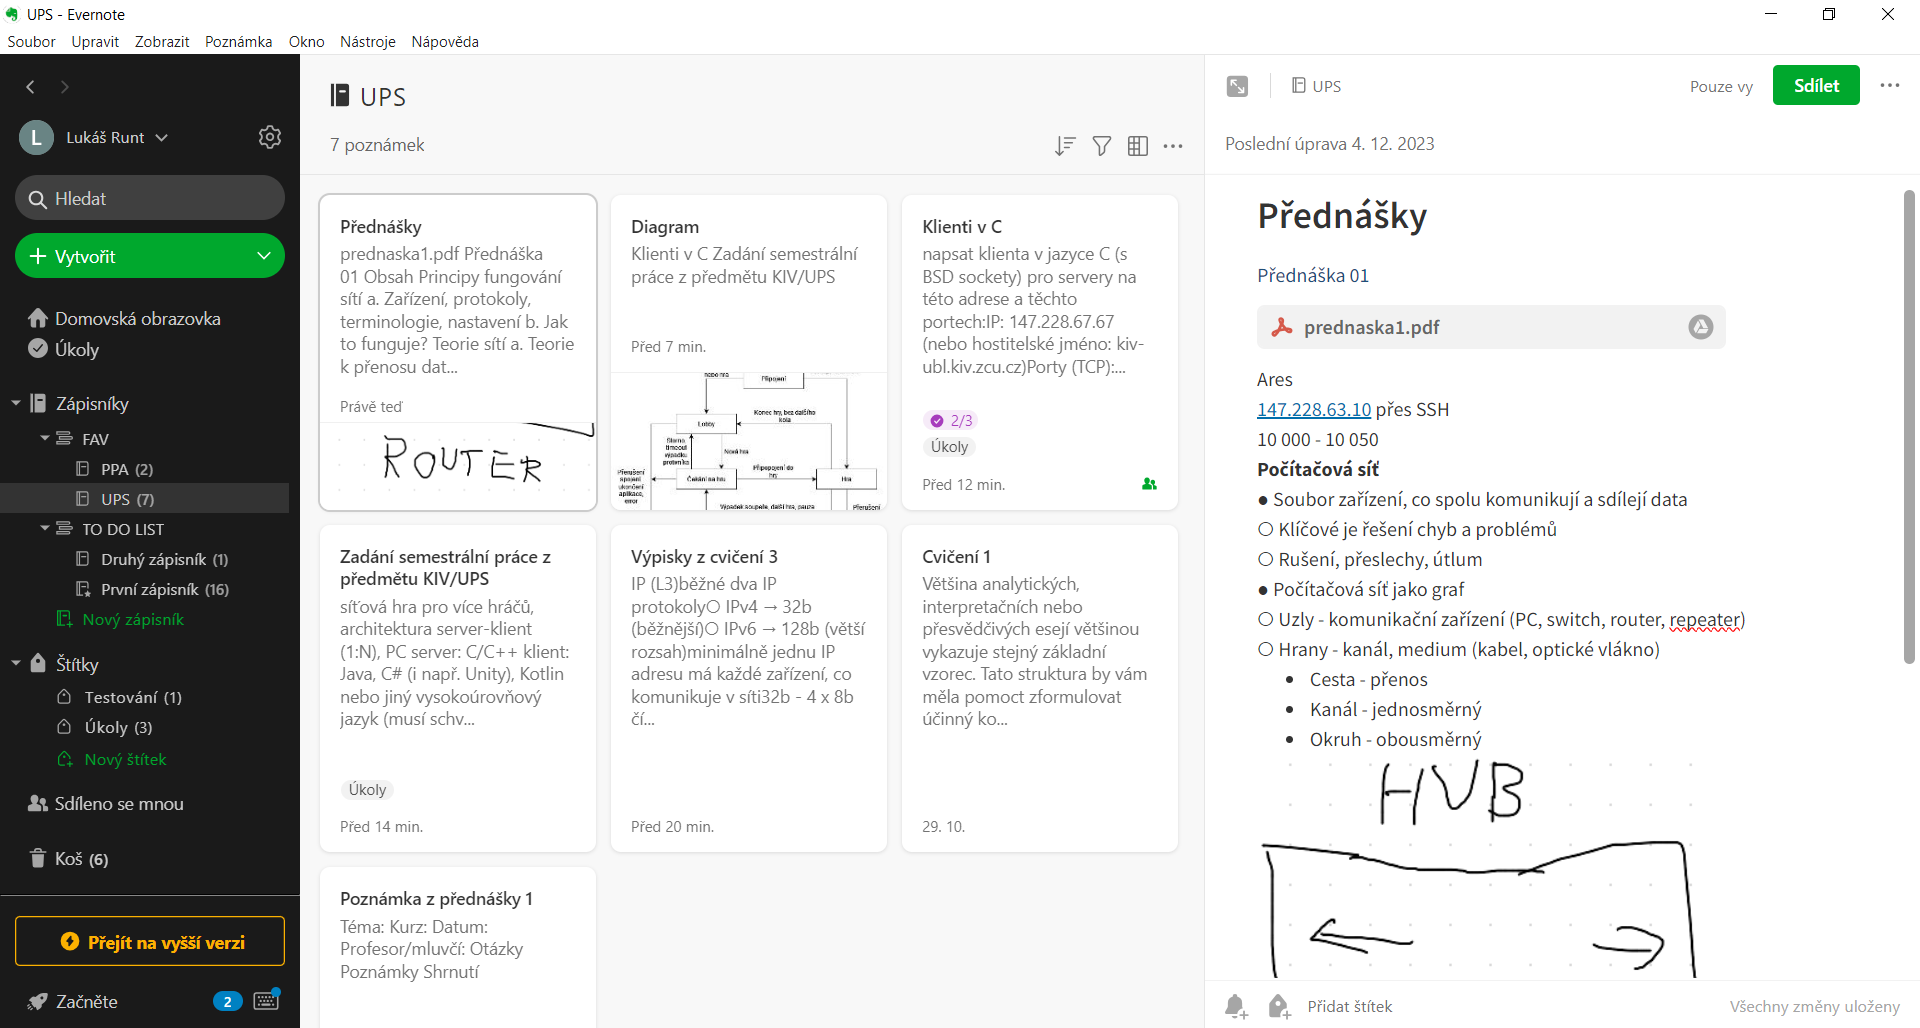
\includegraphics[width=1\textwidth]{img/BP-Runt/Evernote/Evernote_PC.PNG}
  \caption{Počítačová verze aplikace Evernote}
  \label{fig:evernote_on_pc}
\end{figure}

\newpage

Evernote nabízí čtyři verze předplatného Free, Personal, Professional a~Teams. Základní verze je bezplatná, avšak je pro uživatele velmi limitující. V~bezplatné verzi můžeme synchronizovat své poznámky jen mezi dvěma zařízeními (web se~počítá jako jedno zařízení), poznámky se dají stahovat pro offline použití pouze na počítači\footnote{Aplikace uchovává v paměti jen poznámky, které jsme zobrazili nebo upravili. S placenou verzí můžeme zvolit, které poznámky budou staženy pro režim bez připojení k internetu.}, omezeny jsou funkce vyhledávání v \gls{PDF} souborech a obrázcích, měsíční upload dat je omezen na 60~MB a maximální velikost poznámky na 25~MB a tím bohužel výčet ani zdaleka nekončí. Ceny prémiových účtů se pohybují od 12,99~€/měsíčně\footnote{Cena předplatného k 19.~11.~2023}.

Aplikace umožňuje vytvářet poznámky a úkoly. Do obsahu poznámek a úkolů je možné vkládat formátovaný text, skici, obrázky, soubory i zvukové nahrávky. Při vytváření nových poznámek lze využít předdefinovaných šablon. Poznámky lze~organizovat pomocí štítků, zkratek a hierarchické struktury, která je zobrazena seznamem a stromovou strukturou ve~vysouvacím menu (viz obrázek \ref{fig:hierarchie_Evernote}). Maximální hloubka hierarchie je omezena na tři úrovně. Pro každou úroveň je definován jeden typ souboru, a~to svazek (úroveň 1), zápisník (úroveň 2) a~poznámka (úroveň 3). Vzhledem k~tomu, že soubory existují pouze v~rámci své vlastní úrovně, není možné vložit soubor stejného typu do identického typu souboru.     

\begin{figure}[h!]
  \centering
  \begin{minipage}[h]{0.3\textwidth}
    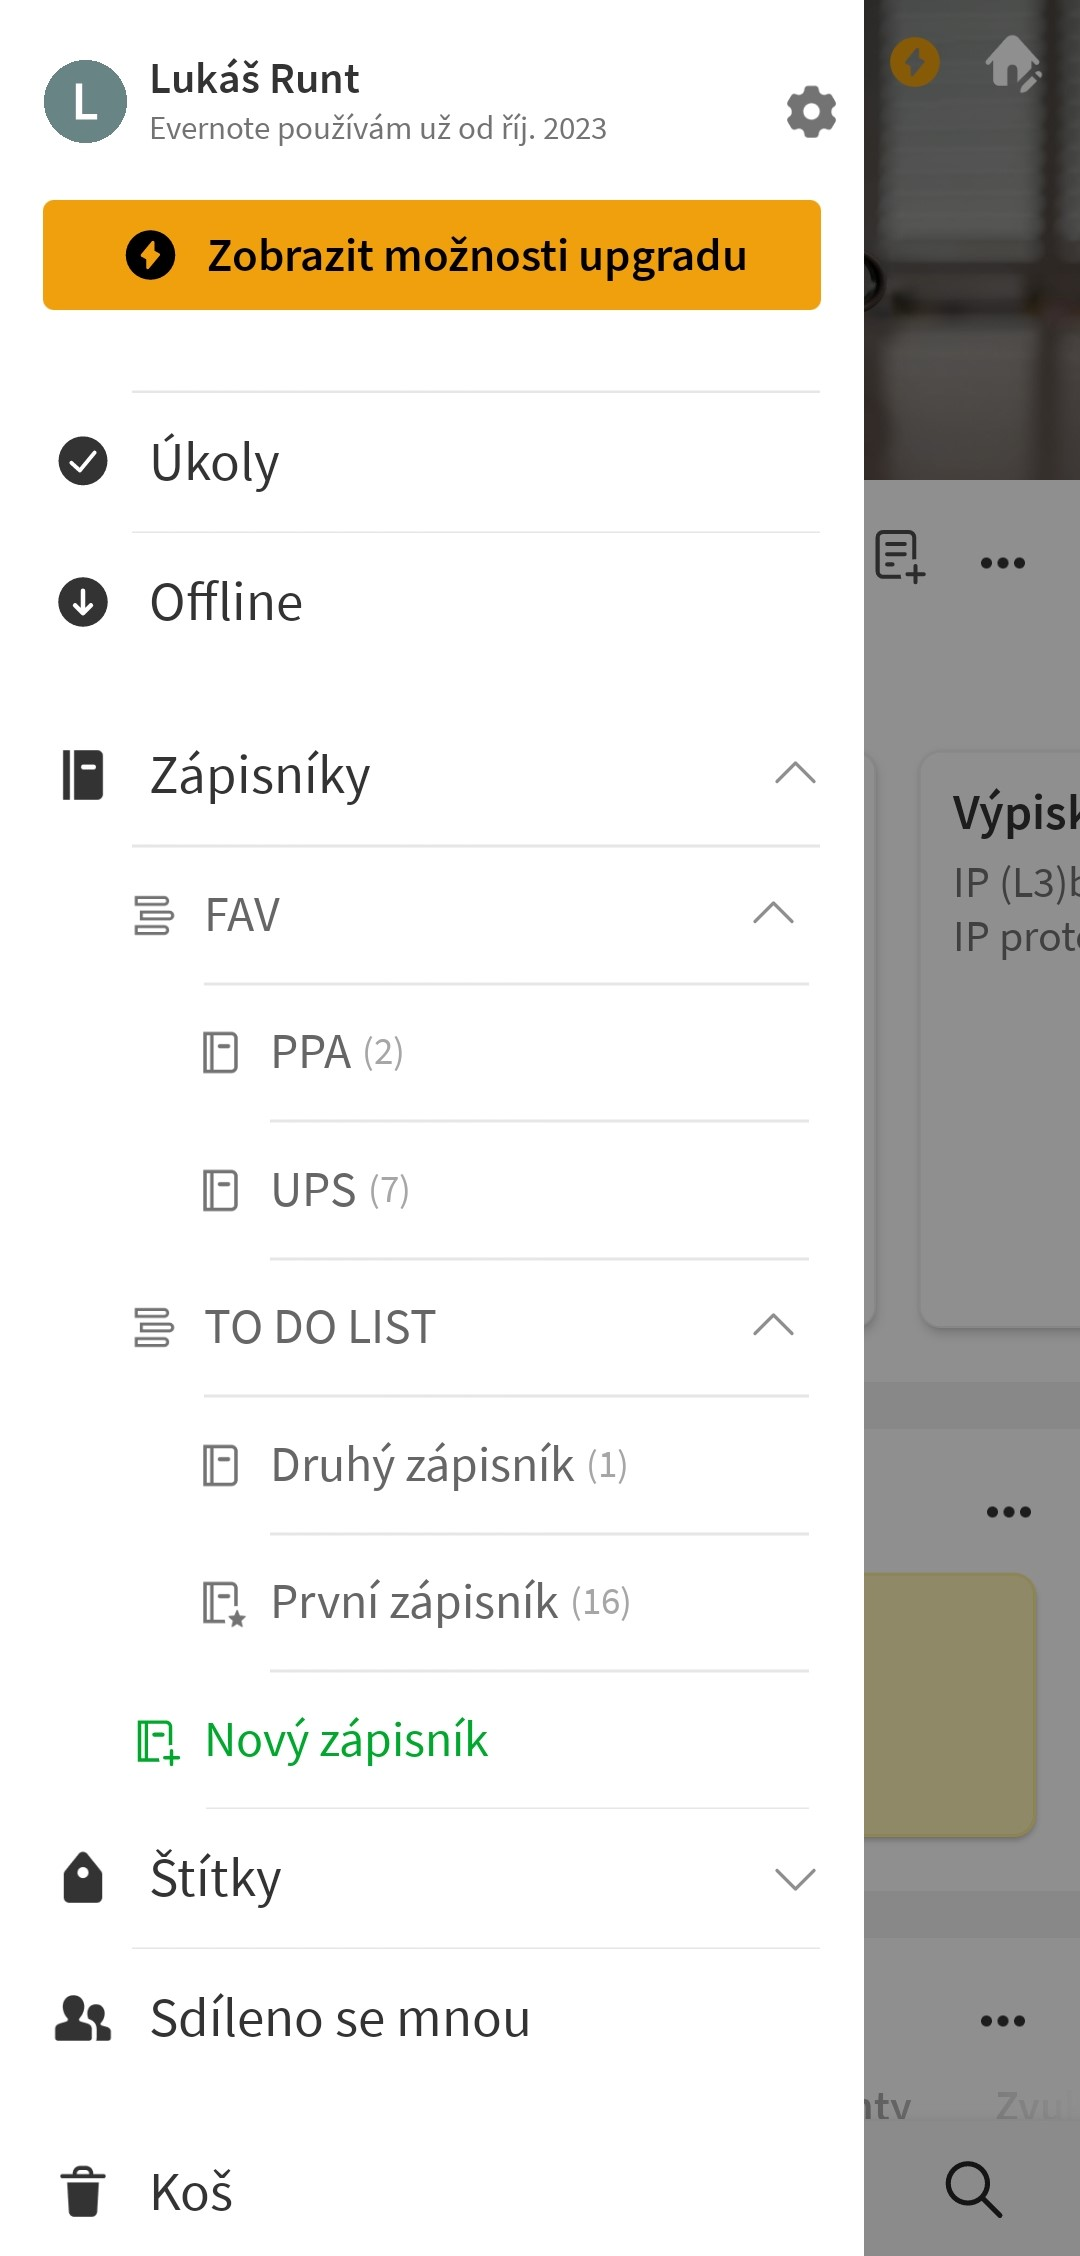
\includegraphics[width=\textwidth]{img/BP-Runt/Evernote/Evernote_hierarchie_v_liste.jpg}
  \end{minipage}
  \hfill
  \begin{minipage}[h]{0.3\textwidth}
    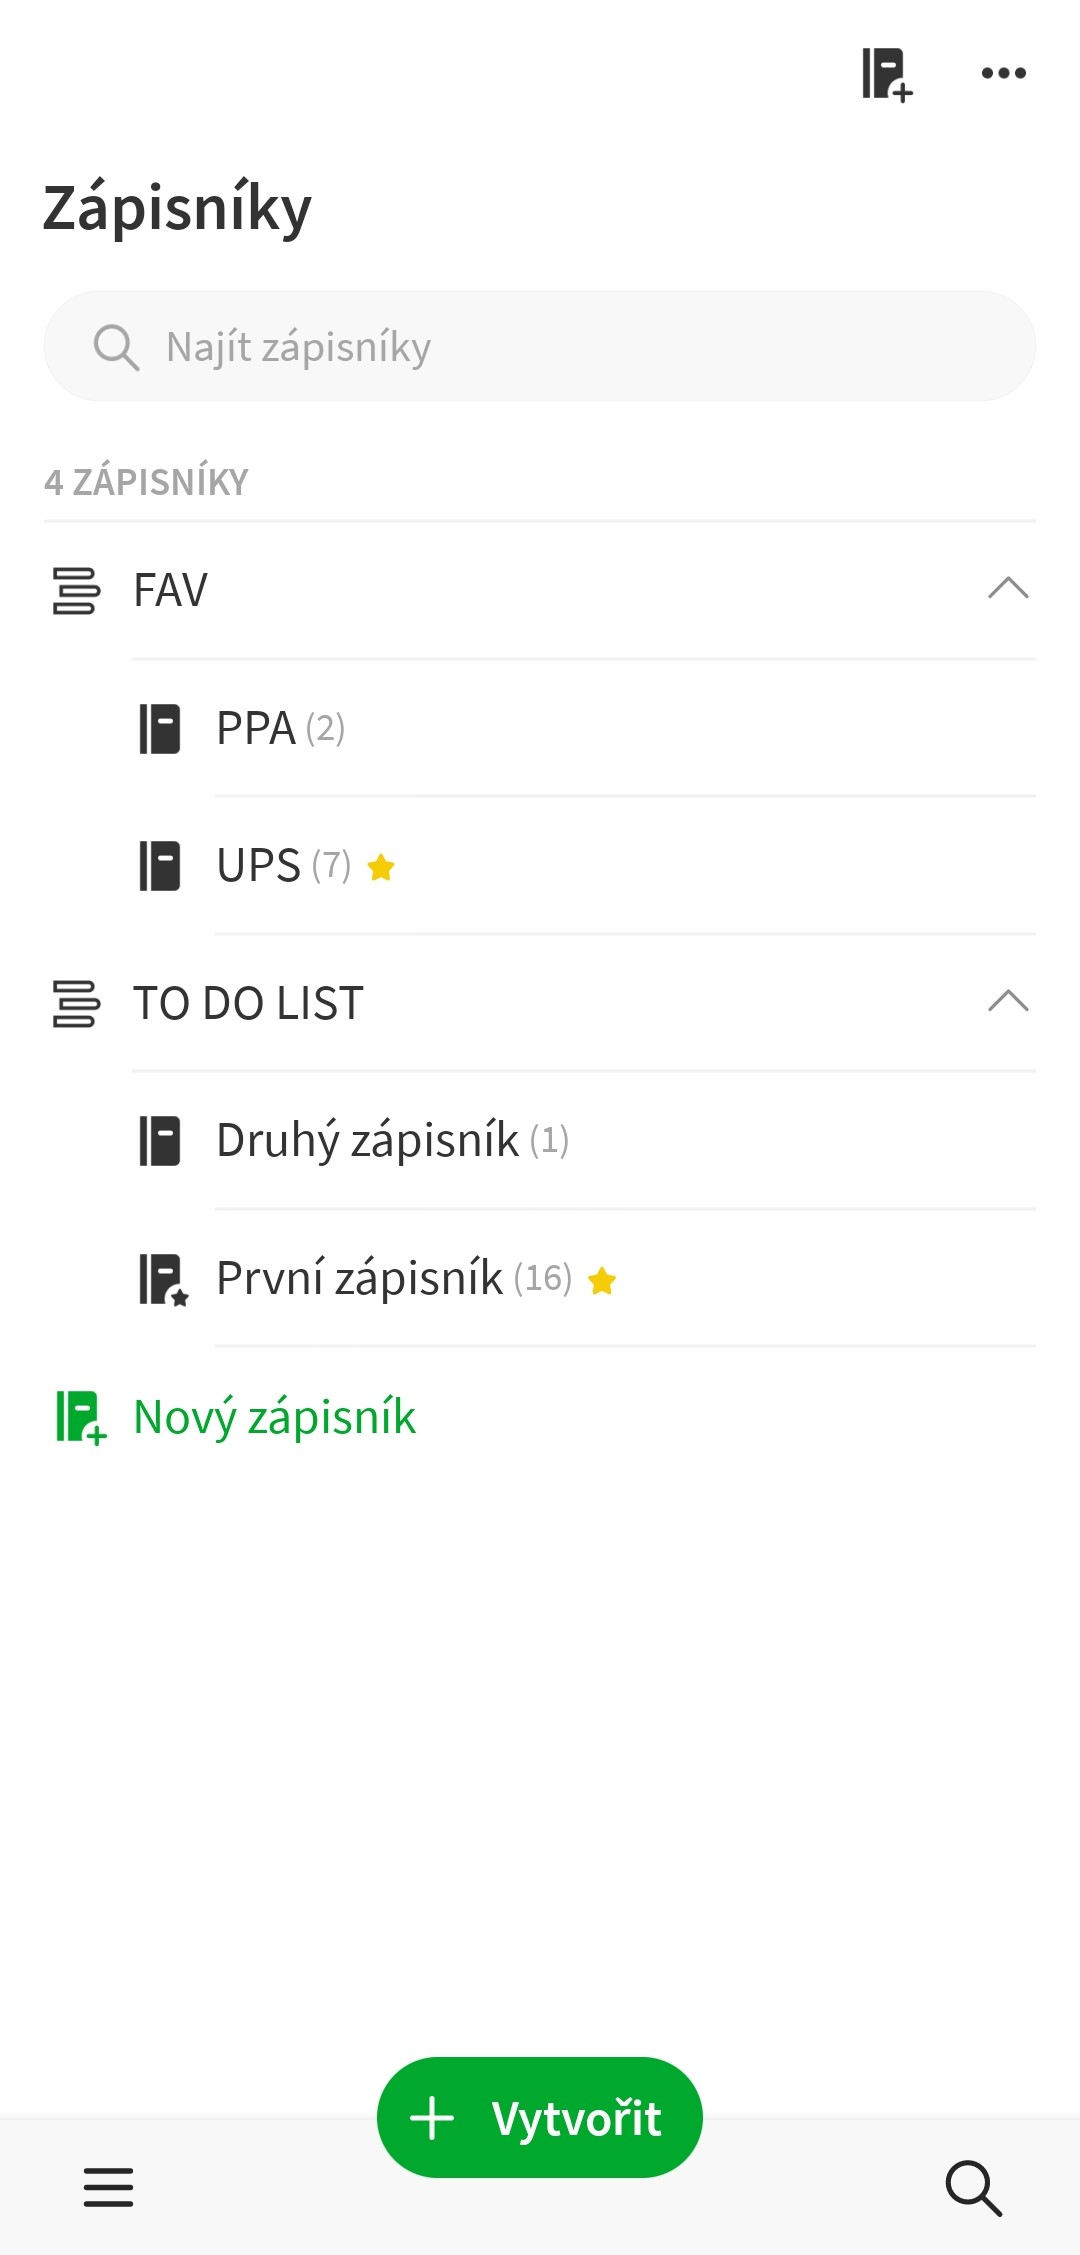
\includegraphics[width=\textwidth]{img/BP-Runt/Evernote/Evernote_hierarchie_v_seznamu.jpg}
  \end{minipage}
  \hfill
  \begin{minipage}[h]{0.3\textwidth}
    \includegraphics[width=\textwidth]{img/BP-Runt/Evernote/Evernote_poznámky.jpg}
  \end{minipage}
  \caption{Organizace poznámek v mobilní aplikaci Evernote. Lišta se stromovou strukturou (vlevo), seznam se zápisníky (uprostřed), seznam poznámek (vpravo)}
  \label{fig:hierarchie_Evernote}
\end{figure}

\newpage

Synchronizace poskytuje uživatelům přístup ke svým poznámkám z~více zařízení. Evernote využívá real-time synchronizaci, tedy změny provedené na jednom zařízení se okamžitě promítají na ostatní zařízení. Uživatelé mohou své poznámky upravovat i bez připojení k internetu. Jakmile je připojení k~internetu obnoveno, provedené změny jsou automaticky synchronizovány. Kromě synchronizace mezi zařízeními lze také sdílet data mezi účty. Sdílet můžeme zápisníky a poznámky pomocí odkazu nebo poslání pozvánky. V rámci sdílení je možné nastavovat práva ostatním uživatelům. Kdo může data zobrazit, editovat a~rozesílat pozvánky. Všechna data jsou uložena na interních serverech společnosti Evernote. Bezpečnost dat při přenosu mezi zařízeními je zajištěna moderními průmyslovými standardy šifrování \gls{TLS}, \gls{SSL} a~\gls{HSTS}.

Evernote se snaží vytvořit uživatelsky přívětivé a produktivní prostředí. Každý uživatel má možnost editace domovské stránky, organizace dat, vytváření štítků a~zkratek. Rychlejší vyhledávání požadovaných informací ulehčuje řazení, filtrování, standardní vyhledávání, vyhledávání v dokumentech a obrázcích s použitím metod \gls{OCR} a vyhledávání s~použitím umělé inteligence, které vrací odpovědi na dotazy psané v přirozeném jazyce. Umělá inteligence je~obsažena také ve funkci AI Note Cleanup, která formátuje, opravuje chyby a upravuje věty, přičemž zanechává původní význam. Myšlenky lze rychle zachytit bez otevření aplikace díky rychlým poznámkám, webovému rozšíření pro ukládání a vytváření výstřižků webových stránek, vestavěné funkci fotoaparátu a nahrávání hlasu. Dále aplikace nabízí notifikace a několik druhů widgetů, které se dají přidat na plochu. Při práci uživatelé rovněž ocení historii změn poznámek. Tato funkce umožňuje sledovat historii úprav a vrátit se k libovolné verzi, nebo obnovit smazaný soubor.

Bohatý je také počet integrací s~ostatními aplikacemi. Uživatelé mohou propojit například Google Disk a Dropbox, pro vkládání souborů přímo z cloudu. Uživatelé s~předplatným mohou spojit aplikaci se svým kalendářem a e-mailovým účetem, čímž získat možnost sledovat a aktualizovat události přímo z Evernote. Dále lze~připojit například Microsoft Teams, Trello, Slack, Zapier a další užitečné aplikace.


\section{OneNote}

OneNote je software pro vytváření poznámek od společnosti Microsoft, který je~součástí kancelářského balíku Microsoft Office. V současné době je možné tento software používat bezplatně na všech platformách včetně mobilního zařízení a~webového prohlížeče. Uživatelé bezplatného účtu jsou omezeni 5~GB úložného prostoru služby OneDrive, kterou OneNote používá pro ukládání dat. Pokud uživatel potřebuje větší úložný prostor, je možno zvýšit tento limit na 100~GB za~1,99~\$/měsíčně \cite{OneNote-help}.
 

\begin{figure}[h!]
  \centering
  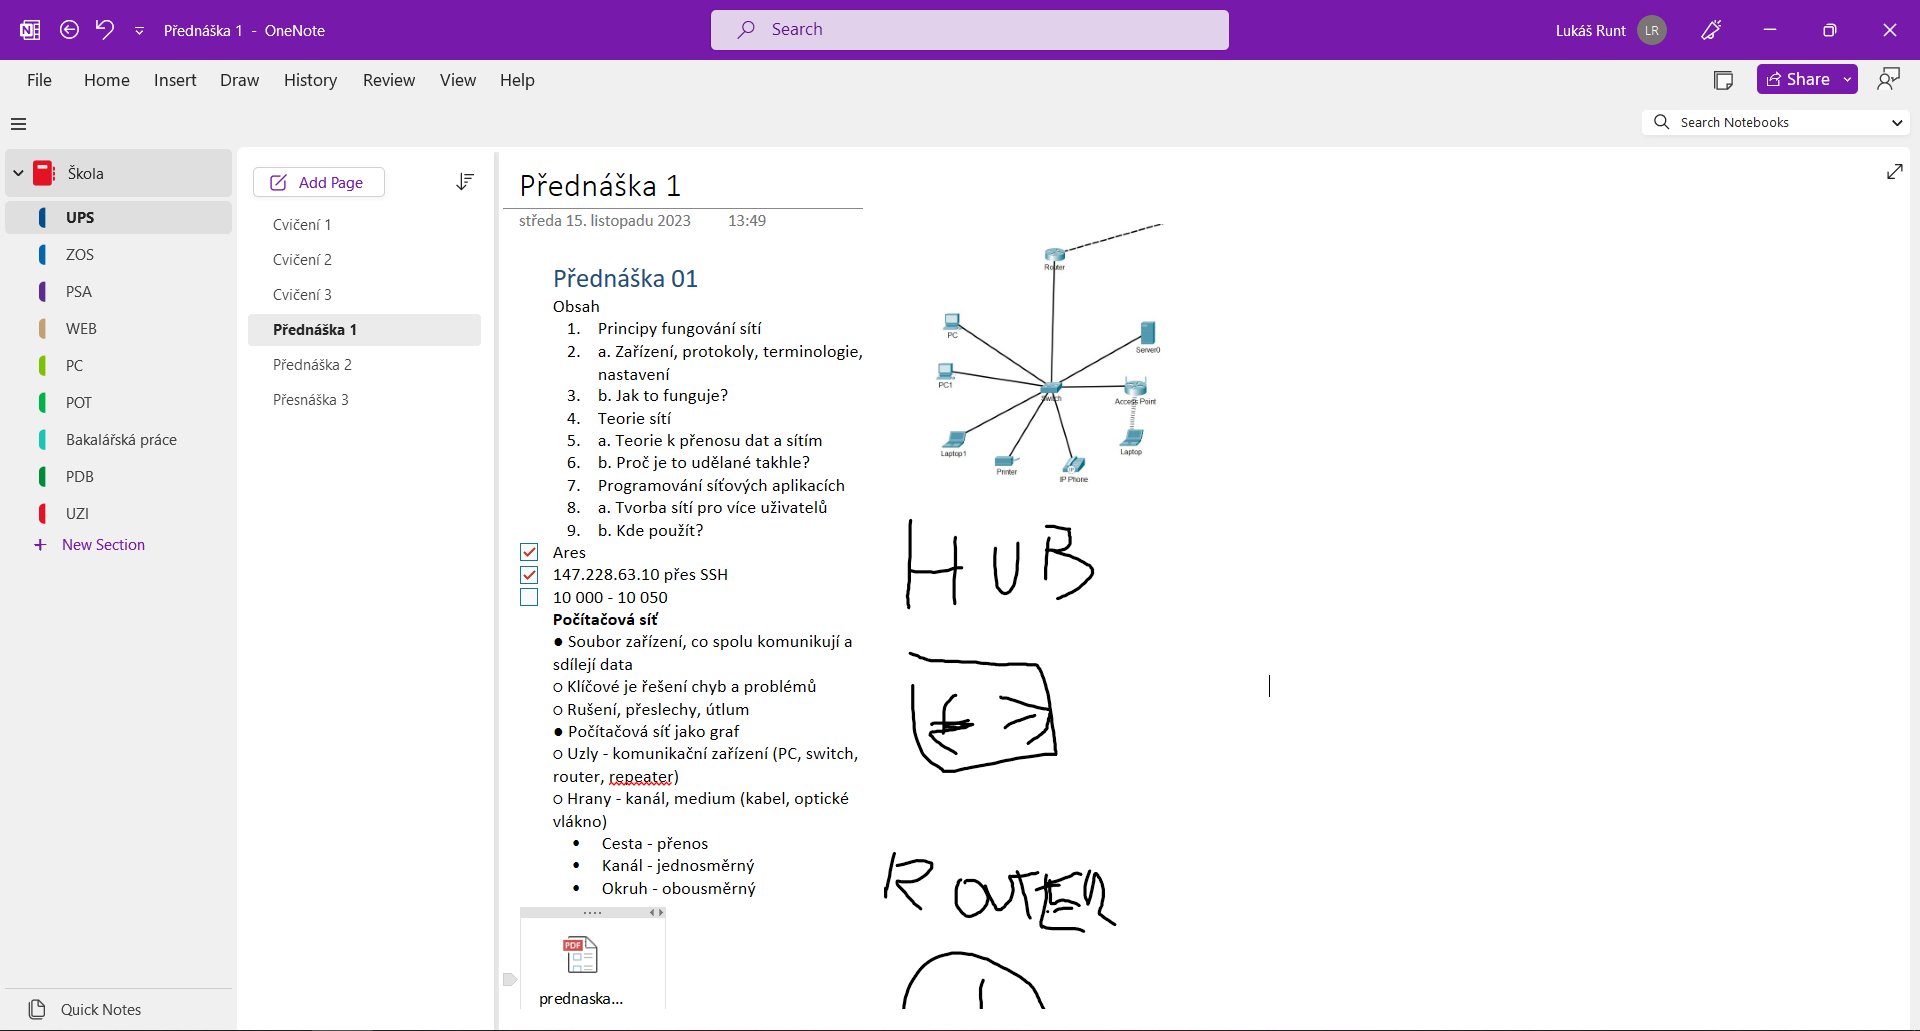
\includegraphics[width=1\textwidth]{img/BP-Runt/OneNote/OneNote_PC.png}
  \caption{Aplikace OneNote na počítači}
  \label{fig:OneNoteOnPc}
\end{figure}

Uživatelské rozhraní aplikace OneNote připomíná ostatní produkty od společnosti Microsoft (viz obrázek \ref{fig:OneNoteOnPc}). Při vytváření poznámek máme k dispozici formátování textů, vytváření zaškrtávacích seznamů, vkládání obrázků, souborů, zvukových nahrávek, kreslení skic ani tím výčet nekončí. Poznámky jsou uspořádány do poznámkových sešitů, ve~kterých je možno vytvořit libovolný počet oddílů, v nichž můžeme mít neomezený počet stránek\footnote{Počet stránek a oddílů je omezen velikostí úložného prostoru}. Poznámky je možné organizovat do tří úrovní. Uspořádání poznámek je na počítači a webovém prohlížeči zobrazeno v levé části obrazovky. Na~mobilním zařízení se hierarchií postupně proklikáváme v seznamem (viz obrázek \ref{fig:hierarchie_OneNote}), dokud se nedostaneme k požadované poznámce.

Přesouvání poznámek do~jiných poznámkových bloků a je realizováno tlačítkem Přesunout, které se zobrazí při dlouhém podržení (mobilní zařízení), respektive pravým kliknutím na poznámku (počítač). Následně si vybíráme ze seznamu oddílů a poznámkových bloků, kam bude poznámka přesunuta. Tato funkce dokáže také poznámky kopírovat. Na počítači lze stránky přesouvat přetažením do jiného oddílu. Přesouvání oddílů do jiných poznámkových bloků není umožněno.

%hierarchie na telefonu
\begin{figure}[h!]
  \centering
  \begin{minipage}[h]{0.3\textwidth}
    \includegraphics[width=\textwidth]{img/BP-Runt/OneNote/OneNote_hierarchie_sešity.jpg}
  \end{minipage}
  \hfill
  \begin{minipage}[h]{0.3\textwidth}
    \includegraphics[width=\textwidth]{img/BP-Runt/OneNote/OneNote_hierarchie_oddíl.jpg}
  \end{minipage}
  \hfill
  \begin{minipage}[h]{0.3\textwidth}
    \includegraphics[width=\textwidth]{img/BP-Runt/OneNote/OneNote_hierarchie_stránky.jpg}
  \end{minipage}
  \caption{Hierarchie v mobilní aplikaci OneNote}
  \label{fig:hierarchie_OneNote}
\end{figure}

OneNote poskytuje automatickou synchronizaci v reálném čase a spolupráci mezi více uživateli. Poznámky jsou dostupné i v offline režimu, provedené změny se~synchronizují po připojení k internetu. Synchronizace a ukládání dat probíhá prostřednictvím cloudové služby OneDrive. Uživatelé mají možnost spravovat přístup ostatních uživatelů k jejich poznámkám. Poznámkové bloky a oddíly se dají zabezpečit heslem, což způsobí uzamčení a zašifrování všech stránek, dokud uživatel nezadá správné heslo. Všechny soubory jsou zkontrolovány antivirovou ochranou a~zakódovány unikátním \gls{AES}-256 klíčem. Šifrován je také přenos mezi zařízeními a servery Microsoftu, který využívá protokolu \gls{TLS} a~\gls{HTTPS}. Žádný vývojář nemá přístup k~datům a do datacenter má přístup jen určený personál.

Kromě již zmíněných funkcí nabízí OneNote také widgety na plochu a Web Cliper, který dokáže ukládat články, výstřižky, odkazy a anotovat obsah. Z běžné funkcionality nechybí ani hledání, filtrování, řazení poznámek, historie úprav, vytváření odkazů mezi poznámkami, používání šablon, práce s matematickými vzorci a tabulkami, správa úkolů a podpora citací a další. Pro uživatele dotykových zařízení je k dispozici podpora pera, korekce a rozpoznávání rukou napsaného textu. Přítomné je také rozeznávání textu \gls{OCR} v dokumentech a obrázcích.

Nechybí ani integrace s~dalšími aplikacemi balíčku Microsoft Office, přes aplikaci Newton je možné posílat důležité e-maily a přes Zapier je možné propojit OneNote s~dalšími aplikacemi, jako je Twitter, Google kalendář, Trello a mnohé další.


\section{Joplin}

Joplin je open-source aplikace pro zaznamenávání poznámek a úkolů, jejíž zdrojový kód je veřejně dostupný na platformě GitHub\footnote{\url{https://github.com/laurent22/joplin}} \cite{Joplin-website}. Aplikace je dostupná na~mobilních zařízeních a počítačích (viz obrázek \ref{fig:joplinOnPc}), kde je dostupná i verze bez grafického rozhraní v konzoli. Webová verze není oficiálně k dispozici. Kód aplikace je napsán v~jazycích TypeScript a JavaScript. Zatímco mobilní aplikace je vyvinuta pomocí frameworku React Native, počítačová verze využívá framework Electron. Aplikace Joplin je bezplatná, avšak synchronizace dat prostřednictvím služby Joplin Cloud vyžaduje placené předplatné. Ceny Joplin Cloud se pohybují od 2,99~€ za měsíc.

\begin{figure}[h!]
  \centering
  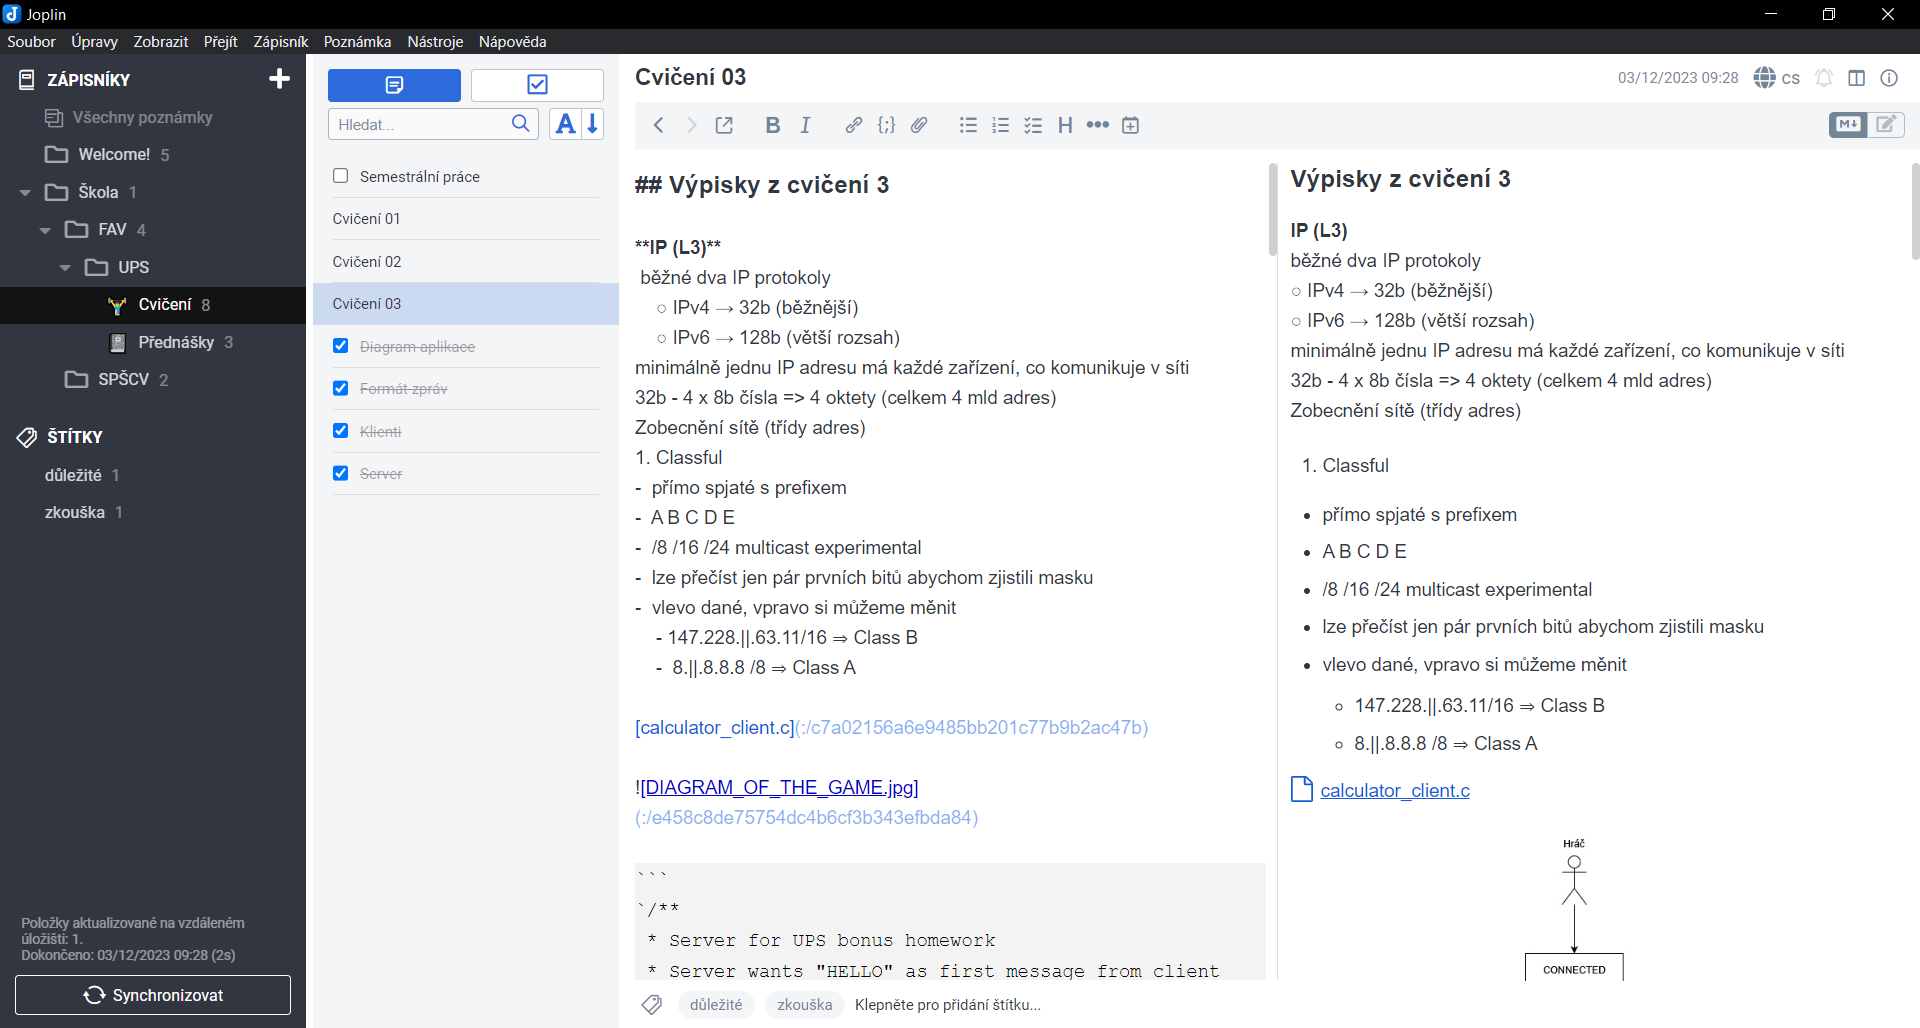
\includegraphics[width=1\textwidth]{img/BP-Runt/Joplin/Joplin_pc.PNG}
  \caption{Aplikace Joplin na počítači}
  \label{fig:joplinOnPc}
\end{figure}

Aplikace nám umožňuje vytvořit poznámky a úkoly. Úkoly se od poznámek liší zaškrtávacím polem, které lze označit jako dokončené. Obsah tvoří formátovaný text s obrázky, soubory a odkazy. Každá poznámka obsahuje také metadata o času a poloze vytvoření, času posledního upravení a verze úprav. Vytváření skic přímo v aplikaci chybí\footnote{Testování probíhalo v aplikaci bez nainstalovaných pluginů}. Poznámky se zobrazují ve dvou režimech, a to v režimu čtení a~režimu úprav. V režimu úpravy si uživatel může přizpůsobit editor podle svého vkusu, jestli má raději \gls{WYSIWYG} editor nebo raději píše text se syntaktickými značkami\footnote{Joplin povoluje více formátu poznámek, mezi které patří například Markdown nebo \gls{HTML}}. Náročnější uživatelé mohou připojit svůj oblíbený textový editor a upravovat v něm poznámky. Poznámky lze organizovat pomocí štítků a hierarchie ve stromové struktuře, která je umístěna v levé části obrazovky. Hierarchie obsahuje poznámky a zápisníky a umožňuje libovolný počet úrovní (viz obrázek \ref{fig:hierarchie_Joplin}). Zápisníky plní funkci složek, lze do nich vkládat poznámky i zápisníky. Přesun zápisníků a poznámek je v mobilní verzi aplikace implementován nastavením rodičovského zápisníku ze seznamu. V desktopové verzi je navíc implementováno přesouvání přetahováním souborů ve stromové struktuře.

%hierarchie na telefonu
\begin{figure}[h!]
  \centering
  \begin{minipage}[h]{0.3\textwidth}
    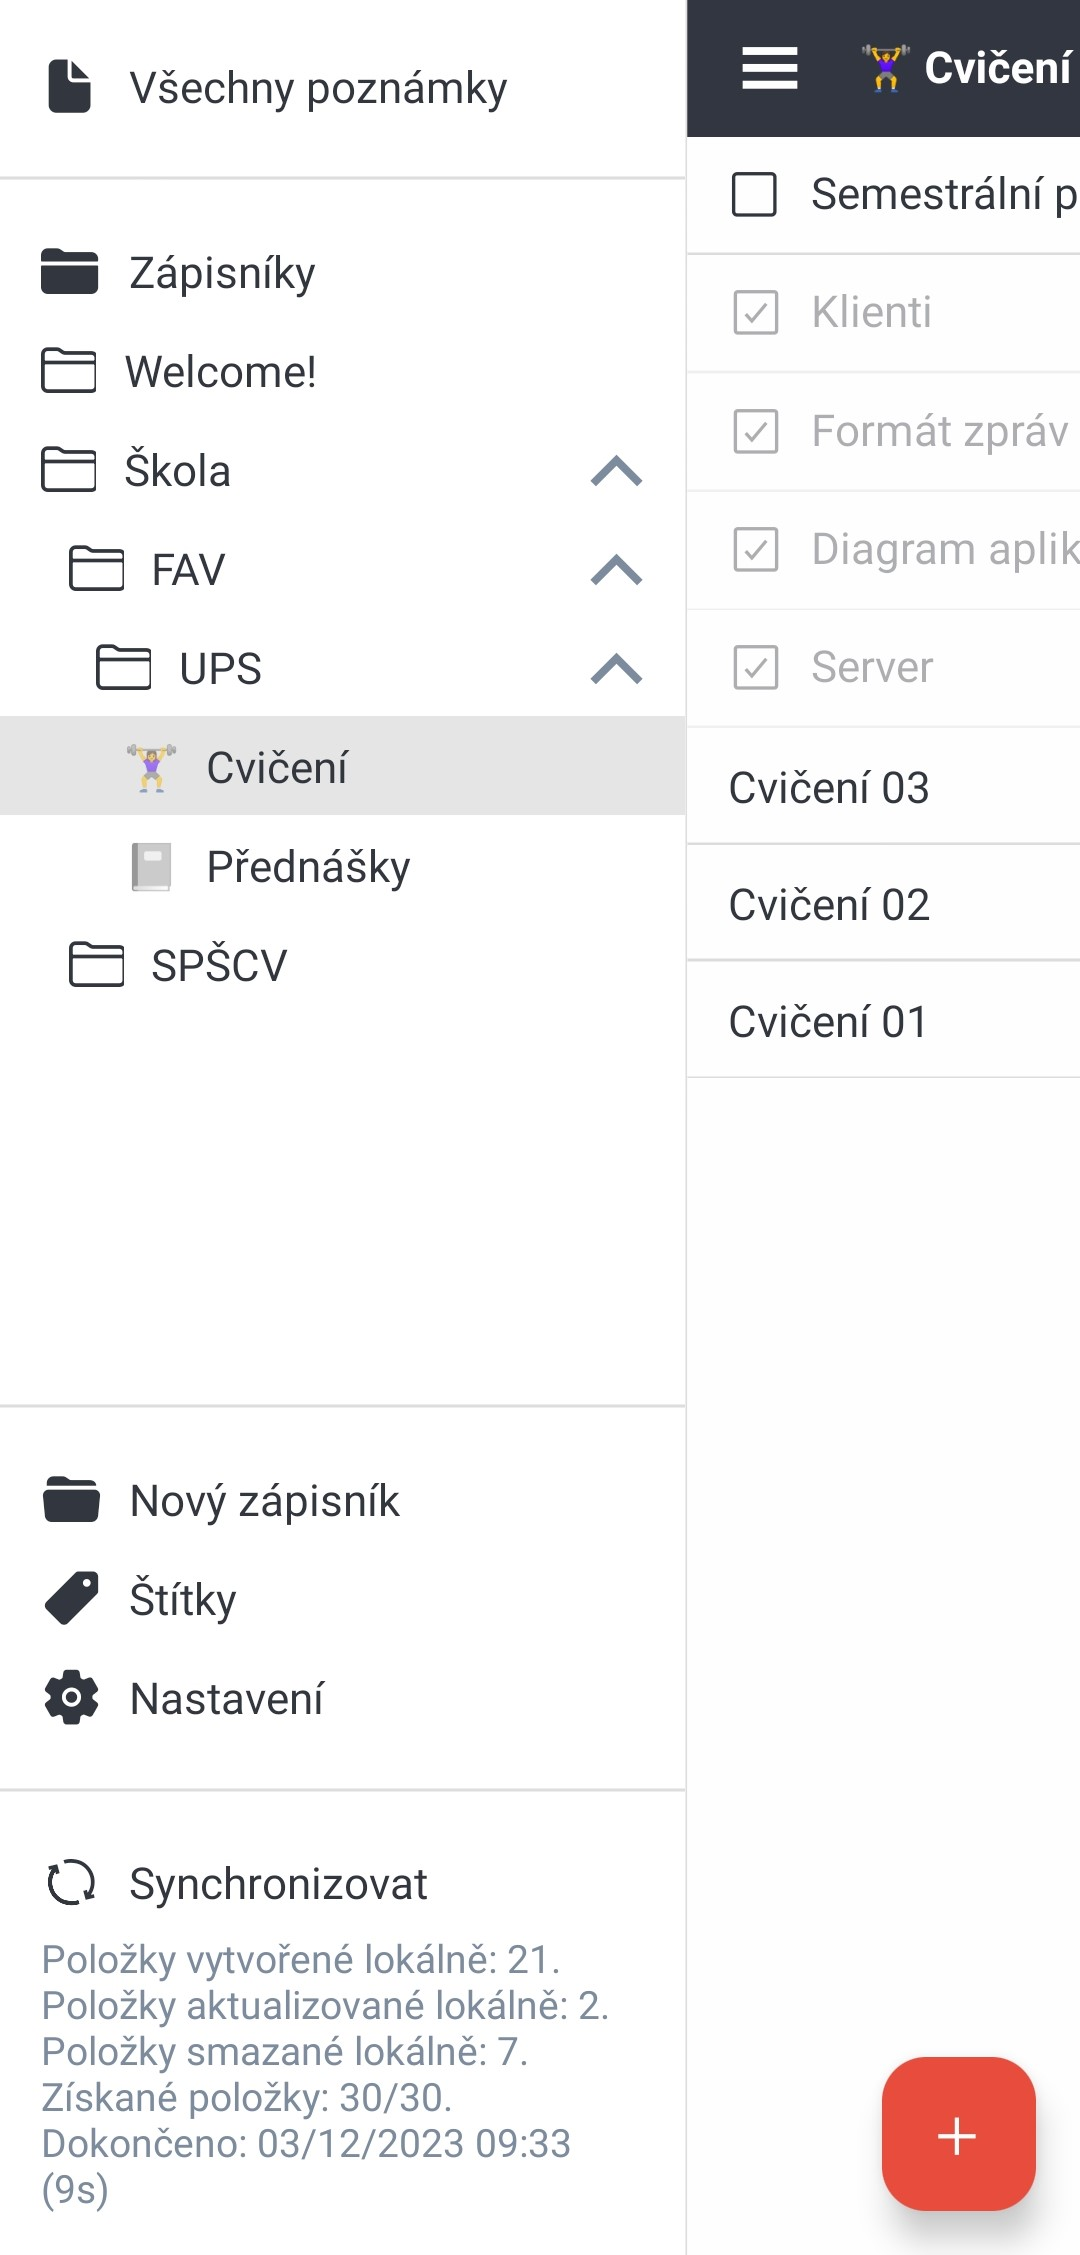
\includegraphics[width=\textwidth]{img/BP-Runt/Joplin/hierarchie_Joplin_telefon.jpg}
  \end{minipage}
  \hspace{30pt}
  \begin{minipage}[h]{0.3\textwidth}
    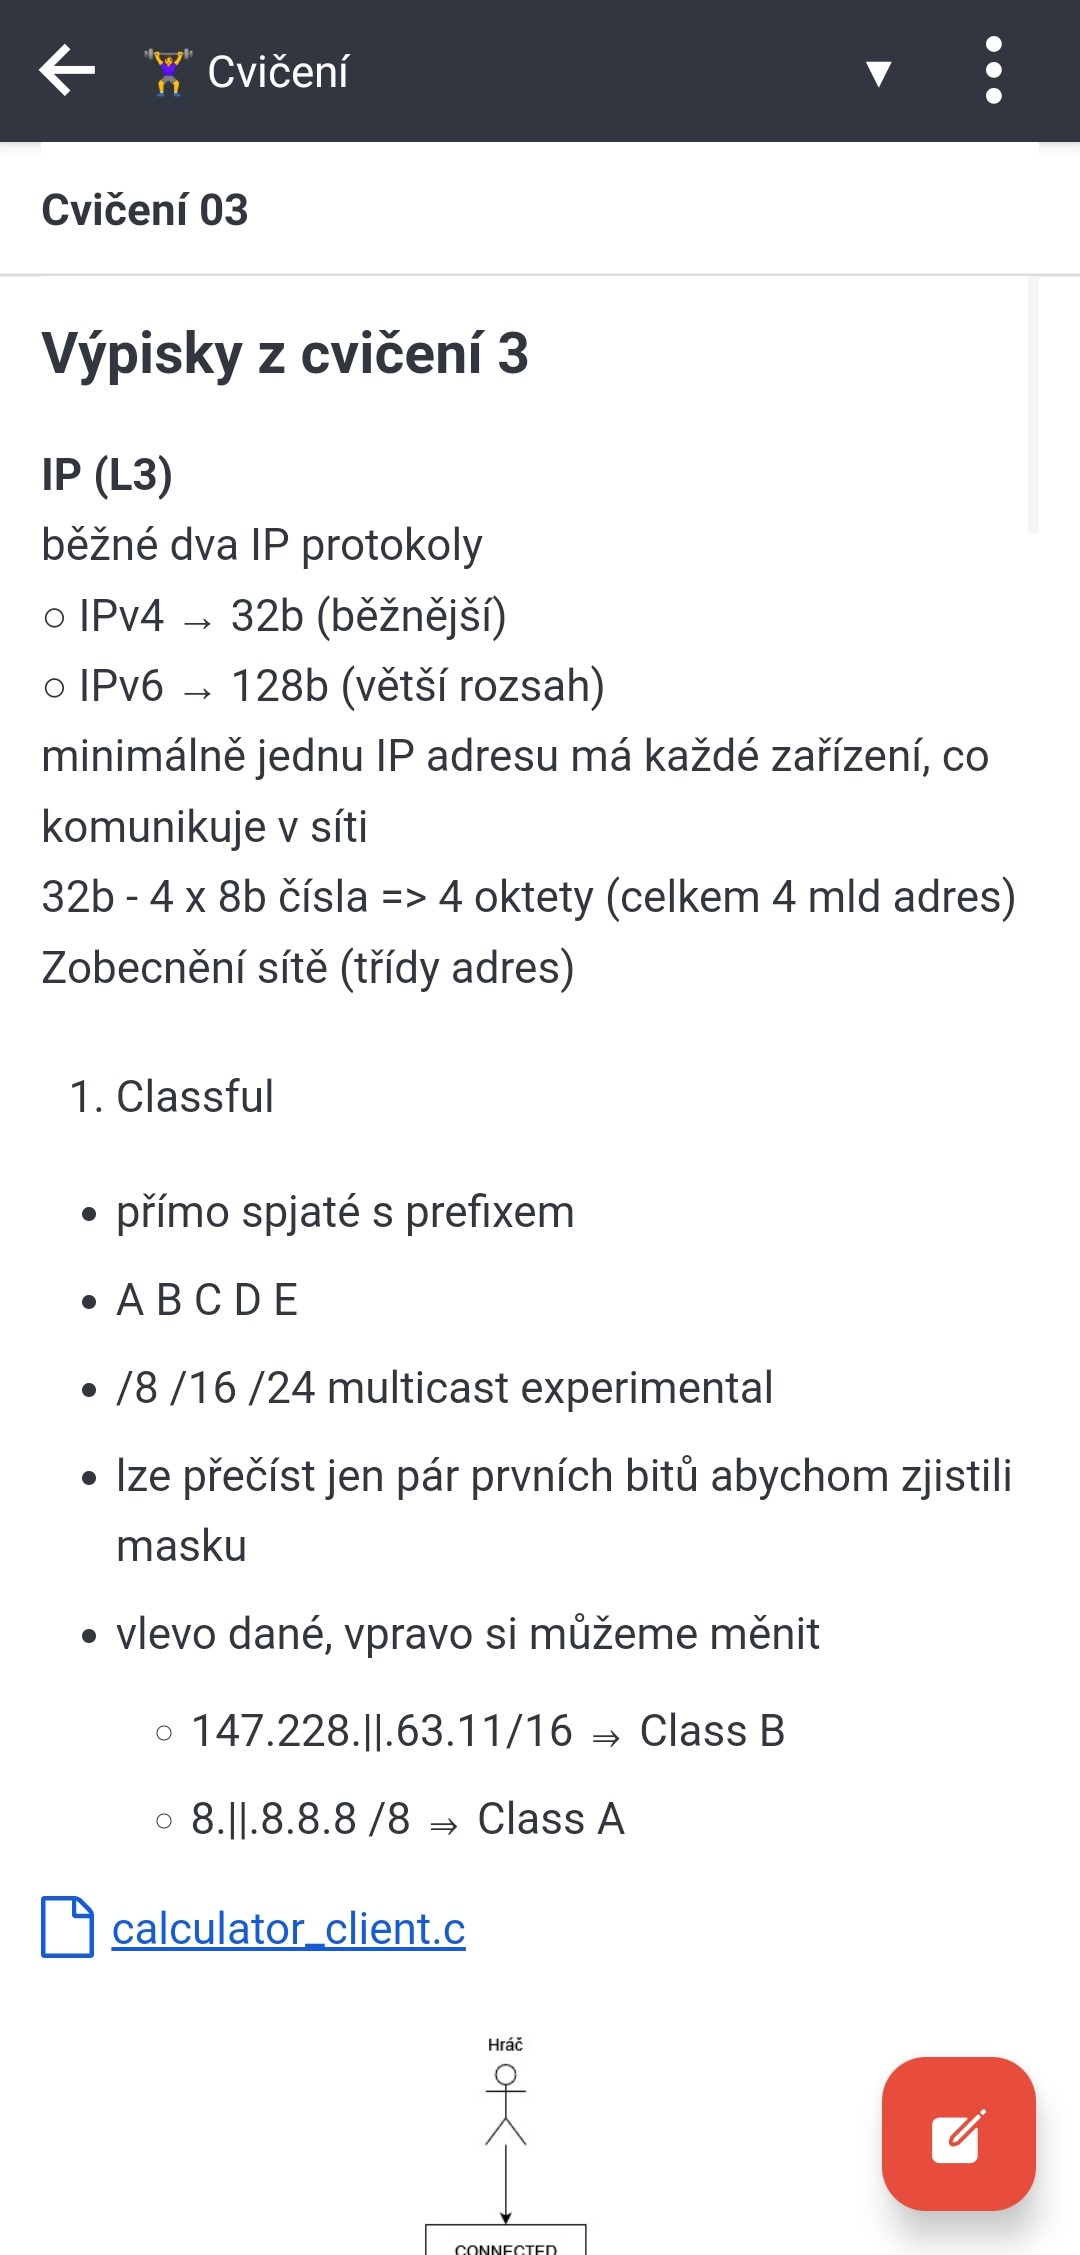
\includegraphics[width=\textwidth]{img/BP-Runt/Joplin/poznamka_Joplin_telefon.jpg}
  \end{minipage}
  \caption{Hierarchická organizace dat (vlevo) a editace poznámky (vpravo)}
  \label{fig:hierarchie_Joplin}
\end{figure}

Primárně je aplikace navržena pro použití bez přístupu k internetu, a tak každé zařízení, na kterém je Joplin nainstalován, uchovává svou vlastní kopii dat. Své poznámky může uživatel také exportovat a importovat v několika možných formátech. Pro automatickou synchronizaci, která se provádí v časových intervalech, si uživatel nastaví časový interval a platformu, na které se budou data ukládat. Je možno zvolit OneDrive, DropBox, NextCloud, Joplin server, Joplin Cloud nebo jinou platformu, kterou Joplin nabízí. Poslední zmiňované služby Joplin Cloud a Joplin Server jsou placené. Oproti ostatním platformám umožňují tyto platformy zveřejnění poznámek na internetu a sdílení dat mezi účty. Vzhledem k časovým intervalům mohou vzniknout při synchronizování dat konflikty, když uživatel současně edituje stejný soubor na více zařízeních. V tomto případě Joplin detekuje konflikt a vytvoří poznámkový blok s konflikty, do kterého nahraje problematické soubory, dále jsou data přepsána. Uživatel si poté může konflikty zobrazit a případně obnovit všechny potřebné změny. Data lze šifrovat koncovým šifrováním, to znamená, že aplikace vygeneruje klíč, kterým jsou data šifrována a dešifrována až u koncového zařízení, na kterém jsou data zobrazována. Šifrování je ve výchozím nastavení vypnuté.

Aplikace obsahuje téměř kompletní českou lokalizaci \footnote{K datu 3. 11. 2023 je přeloženo 96$\%$ textů} a kontrolu českého pravopisu. Vyzdvihnout lze také webové rozšíření pro Firefox a Google Chrome, které umožňuje vytváření výstřižků, ukládání \gls{URL} adres, uložení celé nebo části webu v~několika možných formátování (text, \gls{HTML} a Markdown). V aplikaci nechybí ani řazení, filtrování a hledání v poznámkách. Pokud by uživateli nevyhovoval vzhled nebo ovládání aplikace, může si aplikaci přizpůsobit podle svého vkusu v nastavení. To samé platí i o instalaci a nastavení rozšíření. Vzhledem k tomu, že má Joplin veřejný kód a zveřejněnou vývojářskou dokumentaci na~webových stránkách, má komunita možnost pomoc s vývojem aplikace. V~současné době existuje mnoho rozšíření, které dokáže vylepšit pracovní prostředí Joplinu, jde například o přidání kalendáře, nástrojů pro vytváření diagramů, widgety, podpora \LaTeX, integraci s~aplikacemi a mnoho dalších funkcí.   

\section{Notion}

Notion je multifunkční aplikace s širokým využitím pro spolupráci a organizaci poznámek. Díky rozsáhlé funkcionalitě a integracím s ostatními aplikacemi jde o~opravdu silný nástroj, který lze použít ve firemním prostředí pro řízení projektů a~týmů. Aplikace je dostupná na Windows (viz obrázek \ref{fig:notion_pc}), macOS, iOS, Android a~ve~webovém prohlížeči. \cite{notion-help}

Základní verze aplikace je dostupná zdarma. Náročnější uživatelé si mohou vybrat z tří tarifů předplatného Plus, Business a Enterprise, jejichž cena začíná na~8~\$/Měsíčně. Základní verze nabízí většinu funkcionality, která stačí většině nenáročných uživatelů. Oproti placeným verzím je zde třeba omezena velikost nahraných souborů 5~MB/Soubor, spolupráce s více uživateli, historie úprav, exportování poznámek do PDF formátu a mnohé další. Pokud se tedy očekává práce v~týmu je vhodné si upgradovat na jednu z placených verzí. Studenti a vyučující mohou bezplatně získat některé funkce tarifu plus.

\begin{figure}[h!]
  \centering
  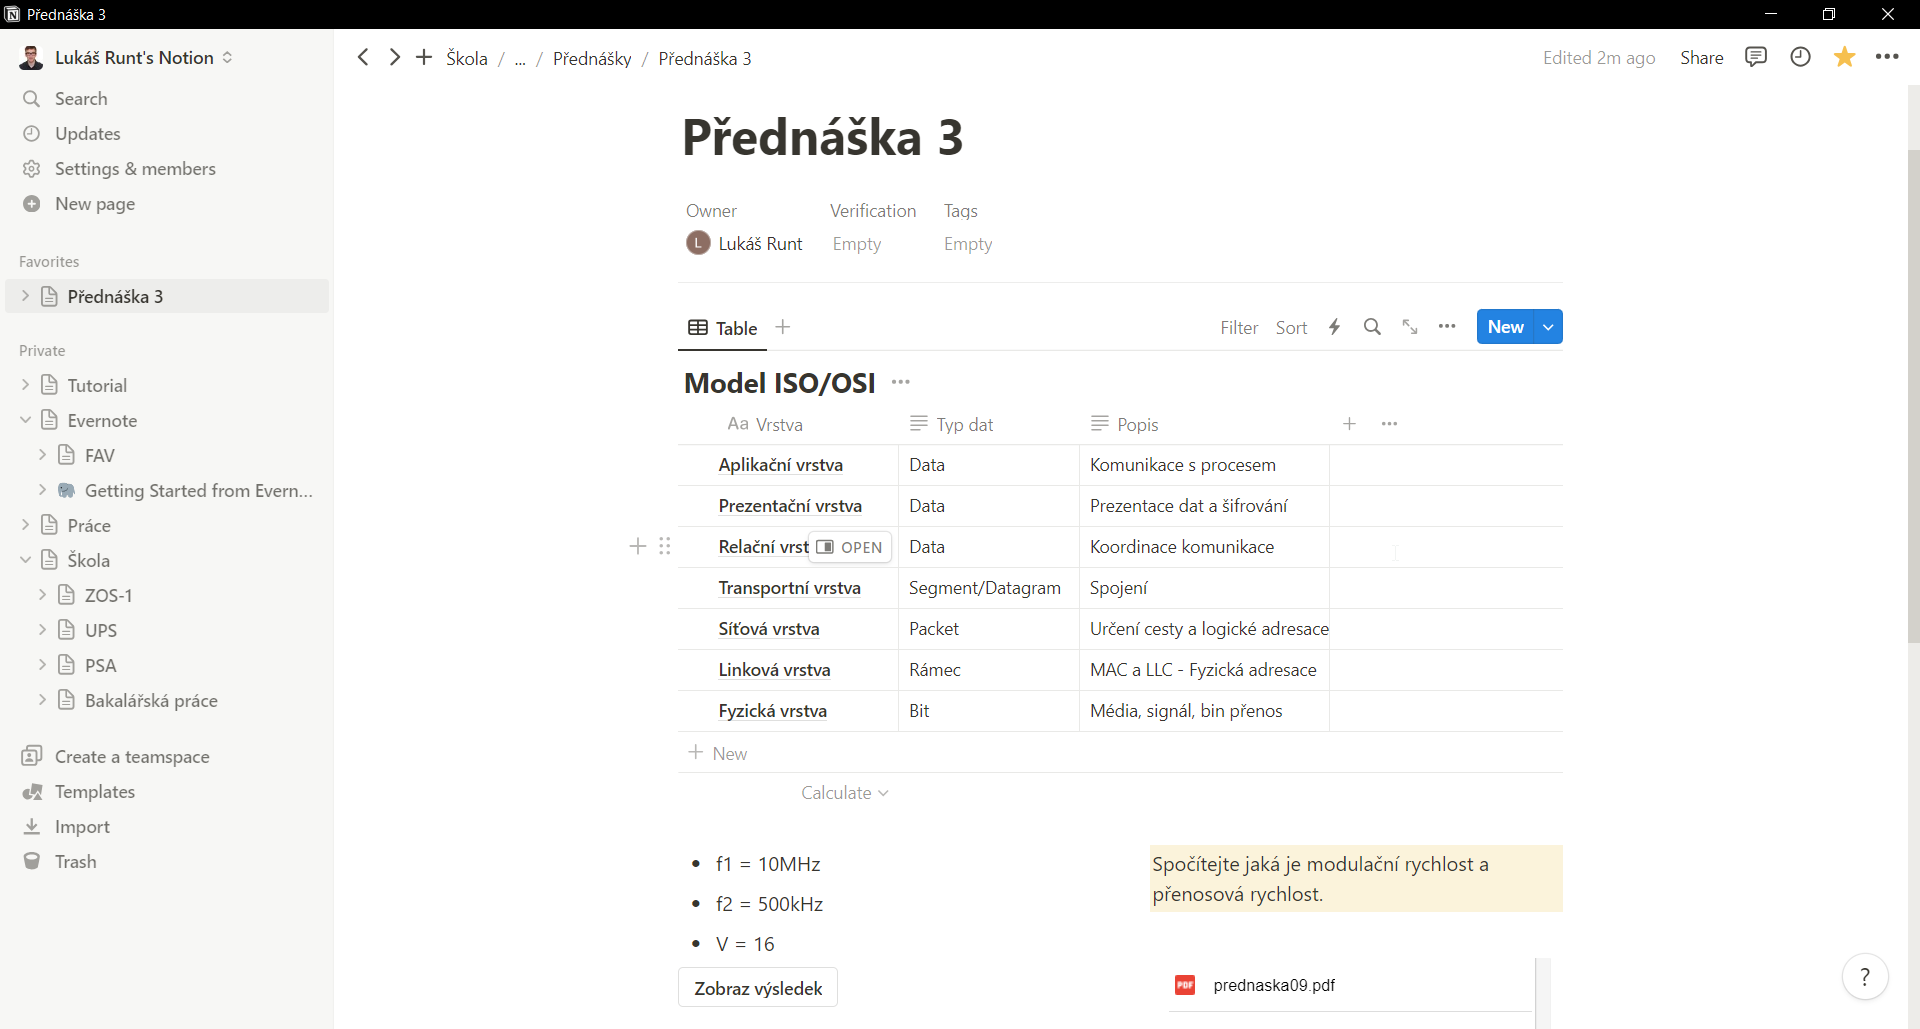
\includegraphics[width=1\textwidth]{img/BP-Runt/Notion/Notion_PC.png}
  \caption{Notion na počítači}
  \label{fig:notion_pc}
\end{figure}

Poznámky se píší a ukládají do stránek. Obsah stránek je strukturován do bloků, které můžeme libovolně uspořádat přetahováním pod sebe, vedle sebe nebo do~sebe. Typ obsahu bloků stránek je velice rozmanitý. Kromě textu, obrázků a videí nabízí také vkládání databází, matematických vzorců, kalendářových bloků, map, internetových stránek, komentářů a další typy obsahů. Do obsahu poznámky lze také vložit další stránku. Tato stránka poté zobrazí v hierarchickém stromě (viz obrázek \ref{fig:hierarchie_Notion}). Hierarchické uspořádání umožňuje libovolný počet úrovní. Uspořádání stránek lze upravovat přetahováním do příslušného místa ve stromě nebo pomocí tří teček u~stránky a následného zvolení „move to", kde si uživatel může vybrat místo, kam bude stránka přesunuta.

\begin{figure}[h!]
  \centering
  \begin{minipage}[h]{0.3\textwidth}
    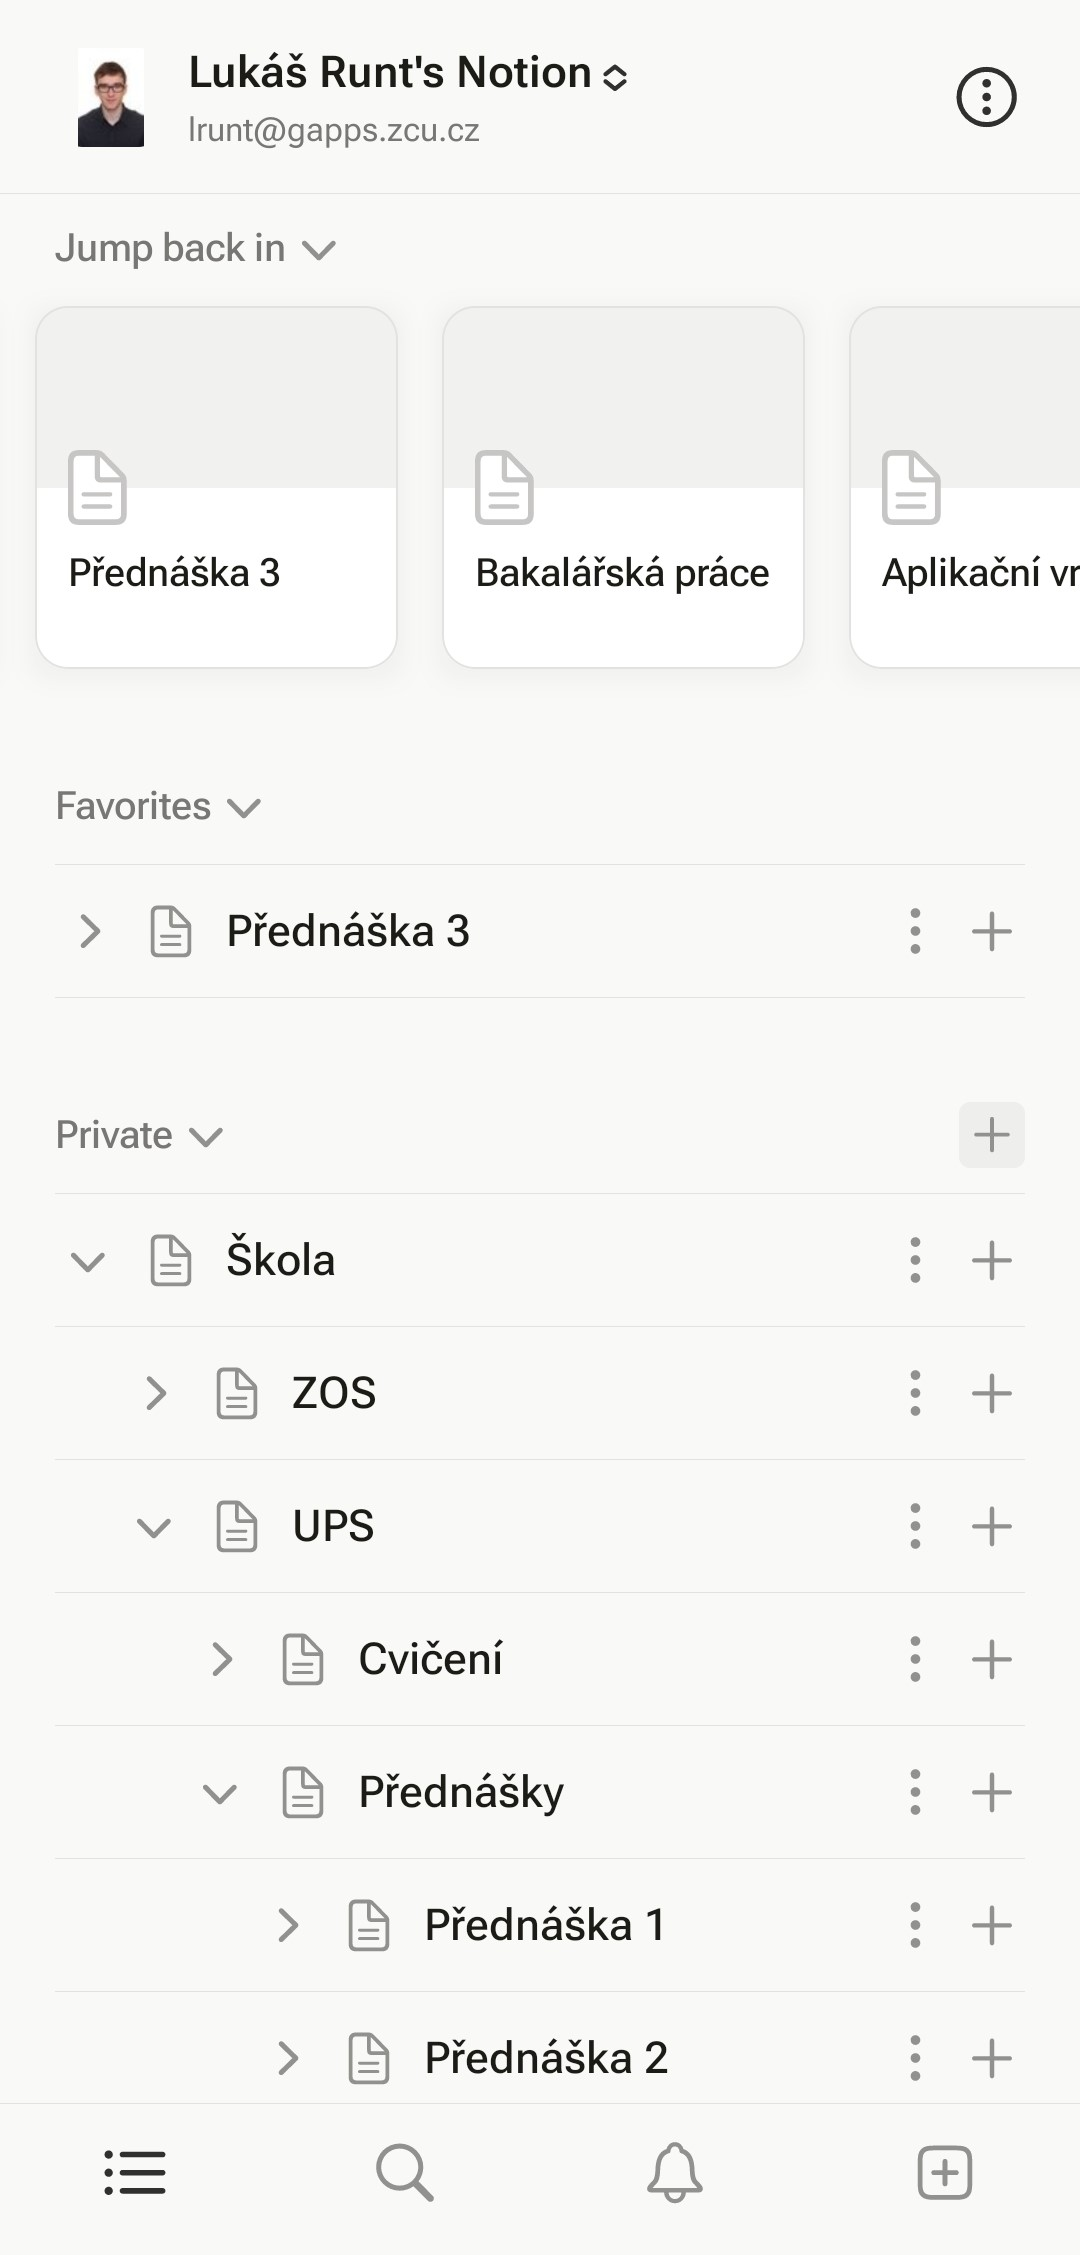
\includegraphics[width=\textwidth]{img/BP-Runt/Notion/Notion_hierarchie.jpg}
  \end{minipage}
  \hspace{30pt}
  \begin{minipage}[h]{0.3\textwidth}
    \includegraphics[width=\textwidth]{img/BP-Runt/Notion/Notion_odkay_na_stránky.jpg}
  \end{minipage}
  \caption{Hierarchická struktura (vlevo) a odkazy na další stránky v obsahu poznámky (vpravo) v mobilní aplikaci Notion}
  \label{fig:hierarchie_Notion}
\end{figure}

Notion je primárně určen pro používání online. Každá změna, kterou uživatel udělá, se automaticky odesílá na cloudovou službu Amazon Web Service, ve které se data ukládají ve formátu \gls{JSON}. Všechna data se~v~reálném čase promítají na všechna ostatní zařízení. Aplikace mimo jiné ukládá data do~ mezipaměti v zařízení uživatele. Do~této paměti se však ukládají jen data poznámek, které uživatel otevřel. Takže pokud chce uživatel prohlížet a~upravovat některou stránku bez připojení k~internetu, musí ji otevřít ještě když má připojení k~internetu a poté nechat aplikaci spuštěnou. Data se po připojení k internetu synchronizují jen za předpokladu, že uživatel nezavřel aplikaci a stránku, ve které proběhlo k~úpravám. V případě, že uživatel stránku zavře nebo obnoví obsah, dojde ke ztrátě dat. Synchronizace není dostupná jen mezi zařízeními, ale je možné sdílet blok i~v~rámci více stránek. Notion nabízí různé úrovně sdílení a práv, které umožňují uživatelům spolupracovat na obsahu a projektech. Sdílené stránky umožňují vytvářet a~sdílet konkrétní stránky a databáze s~ostatními. Pracovní prostory pak poskytují prostředí, kde uživatelé mohou spolupracovat na více projektech s více uživateli. Bezpečnost dat je zajištěna logováním, zálohováním a~šifrováním. Uložená data jsou šifrována algoritmem \gls{AES}-256 a \gls{TLS} při přenosu dat. Pokud dojde k úniku dat, je o~tom uživatel informován do 72 hodin.       

Notion obsahuje opravdu velké množství funkcí a integrací s ostatními aplikacemi, čímž vytváří velmi produktivní pracovní prostředí. Mezi funkcemi nechybí označování štítky, vyhledávání, řazení, historie změn. Jednou z předností aplikace je nespočet různých typů obsahu, které může být uložen na jedné stránce. Jedním z~nestandardních typů jsou databáze, které lze navzájem propojovat, používat v~nich matematické funkce, automatizovat s nimi procesy a zobrazovat je v různých rozdílných zobrazení. Dále v obsahu stránky můžeme vytvořit tlačítka, kterým můžeme nadefinovat akce. V aplikaci je přítomná umělá inteligence pro vygenerování určitého textu, shrnutí bloků a~vyhledávání. Importovat lze data několik formátů a~aplikací. V aplikaci je přítomná kontrola českého pravopisu a~gramatiky Česká lokalizace bohužel není dostupná. Bohatý počet integrací s dalšími nástroji a službami, ať už oficiálními nebo pomocí \gls{API}, poskytuje možnost propojit Notion s externími aplikacemi a~rozšířit tak jeho již existující bohatou funkcionalitu. 

\section{Obsidian}

Obsidian je software pro tvorbu a organizaci poznámek, který se odlišuje od konkurence propojováním poznámek přes odkazy a následné zobrazení vazeb formou grafu (viz obrázek \ref{fig:obsidian_pc}). Aplikace je napsána v jazycích TypeScript a JavaScript s~využitím frameworku Electron. Aplikace je dostupná na mobilních zařízeních a~počítačích. Obsidian je bezplatný pro personální použití. Komerční užití je zpoplatněno 50~\$/rok za každého uživatele. Další placené služby aplikace jsou Obsidian Sync a~Obsidian Publish, které stojí 8\$/měsíc. Obsidian Sync nabízí synchronizování dat do velikosti 10~GB a Obsidian Publish publikaci poznámek na webovou stránku. Poslední placenou položkou je Catalyst, pro předčasný přístup k novým verzím, komunitní odznaky a přístup k VIP kanálu za jednorázovou platbu 25~\$. \cite{obsidian-website}

\begin{figure}[h!]
  \centering
  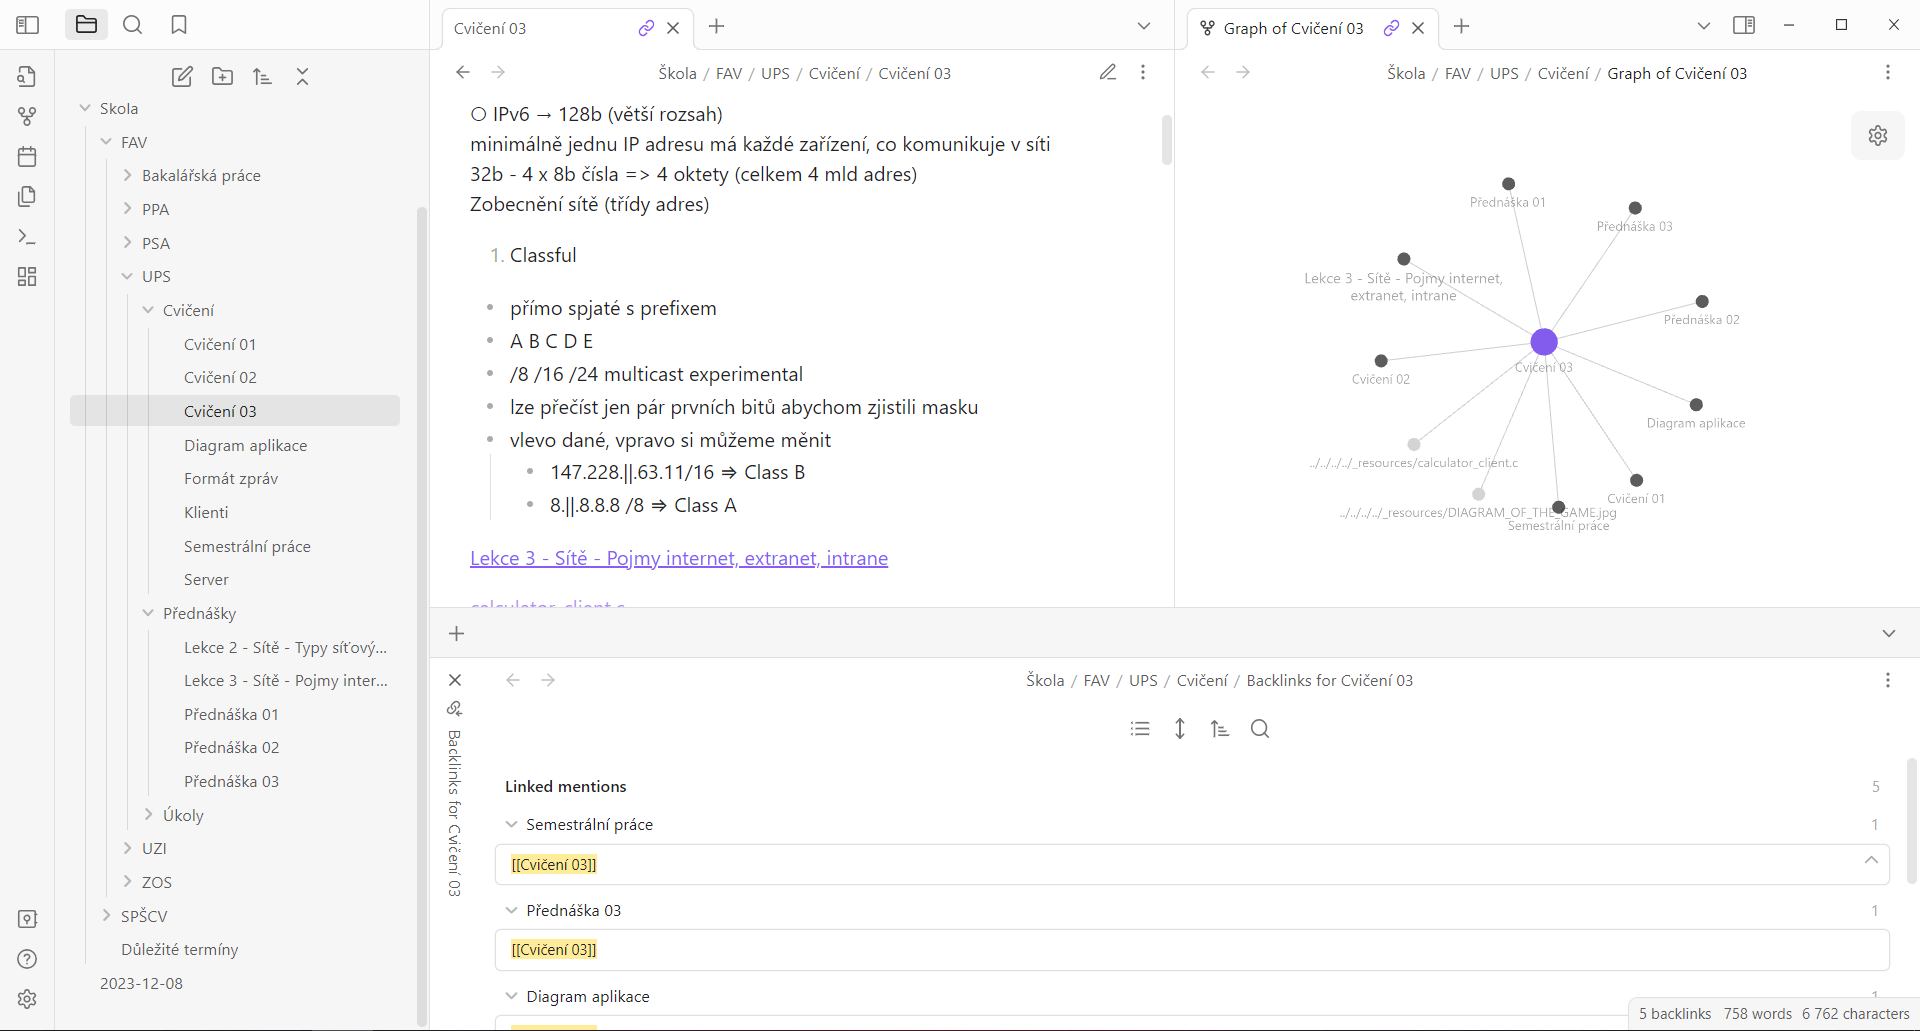
\includegraphics[width=0.90\textwidth]{img/BP-Runt/Obsidian/obsidian_PC2.PNG}
  \caption{Počítačová verze aplikace Obsidian}
  \label{fig:obsidian_pc}
\end{figure}

Aplikace umožňuje vytvářet textové poznámky a plátna (\texttt{canvas}), ve kterých nelze kreslit tužkou. Tato plátna zastupují funkci myšlenkových map. Do plátna lze vkládat textové karty, obrázky a kopie poznámek, které se dají jednoduše propojit šipkami. Do obsahu poznámek je možno vložit formátovaný text, obrázky, \gls{URL} adresy, soubory a odkazy. Vytváření skic přímo v programu chybí. Poznámky i~plátna se dají uspořádat do složek s neomezených počtem úrovní. Strom se~soubory je~zobrazen v levé části obrazovky (viz obrázek \ref{fig:hierarchy_obsidian}). Veškerou manipulaci se~soubory, plátny a poznámkami lze provést pomocí přetažením příslušného souboru do~požadovaného místa ve stromě. Pokud bychom chtěli využít jiný způsob, tak můžeme jednotlivé soubory přesouvat přes podrobnosti o souboru nebo v souborovém systému zařízení.

Obsidian ukládá všechna data ve fyzické paměti zařízení v souborech .md a .canvas, což je speciální formát Obsidianu obsahující \gls{JSON} s informacemi o rozložení a~obsahu karet. Místo, kam se data budou ukládat se nazývá trezor a~uživatel si~jej volí sám. Na místě, které si uživatel zvolí se vytvoří, pokud trezor ještě neexistuje, inicializační složka .obsidian s daty ve formátu \gls{JSON}. Vzhedem k~tomu, že jsou poznámky uložené v paměti zařízení, je možné poznámky upravovat kdykoliv i~bez připojení k internetu, avšak automatická synchronizace je dostupná jen s placenou službou Obsidian Sync. Pokud chce mít uživatel data i~na jiném zařízení, musí všechna data na toto zařízení překopírovat a v aplikaci pak vybrat správnou cestu k trezoru. Při zakoupení Obsidian Sync se pak poznámky synchronizují automaticky v pozadí aplikace a lze je sdílet s ostatními uživateli. V~rámci synchronizace si~můžeme vybrat, které soubory budou při synchronizování ignorovány a~máme k~dispozici historii až rok starých změn. Při synchronizování se data ukládají na~server Obsidianu a~šifrují se koncovým šifrováním s~použitím algoritmu \gls{AES}-256.

\begin{figure}[h!]
  \centering
  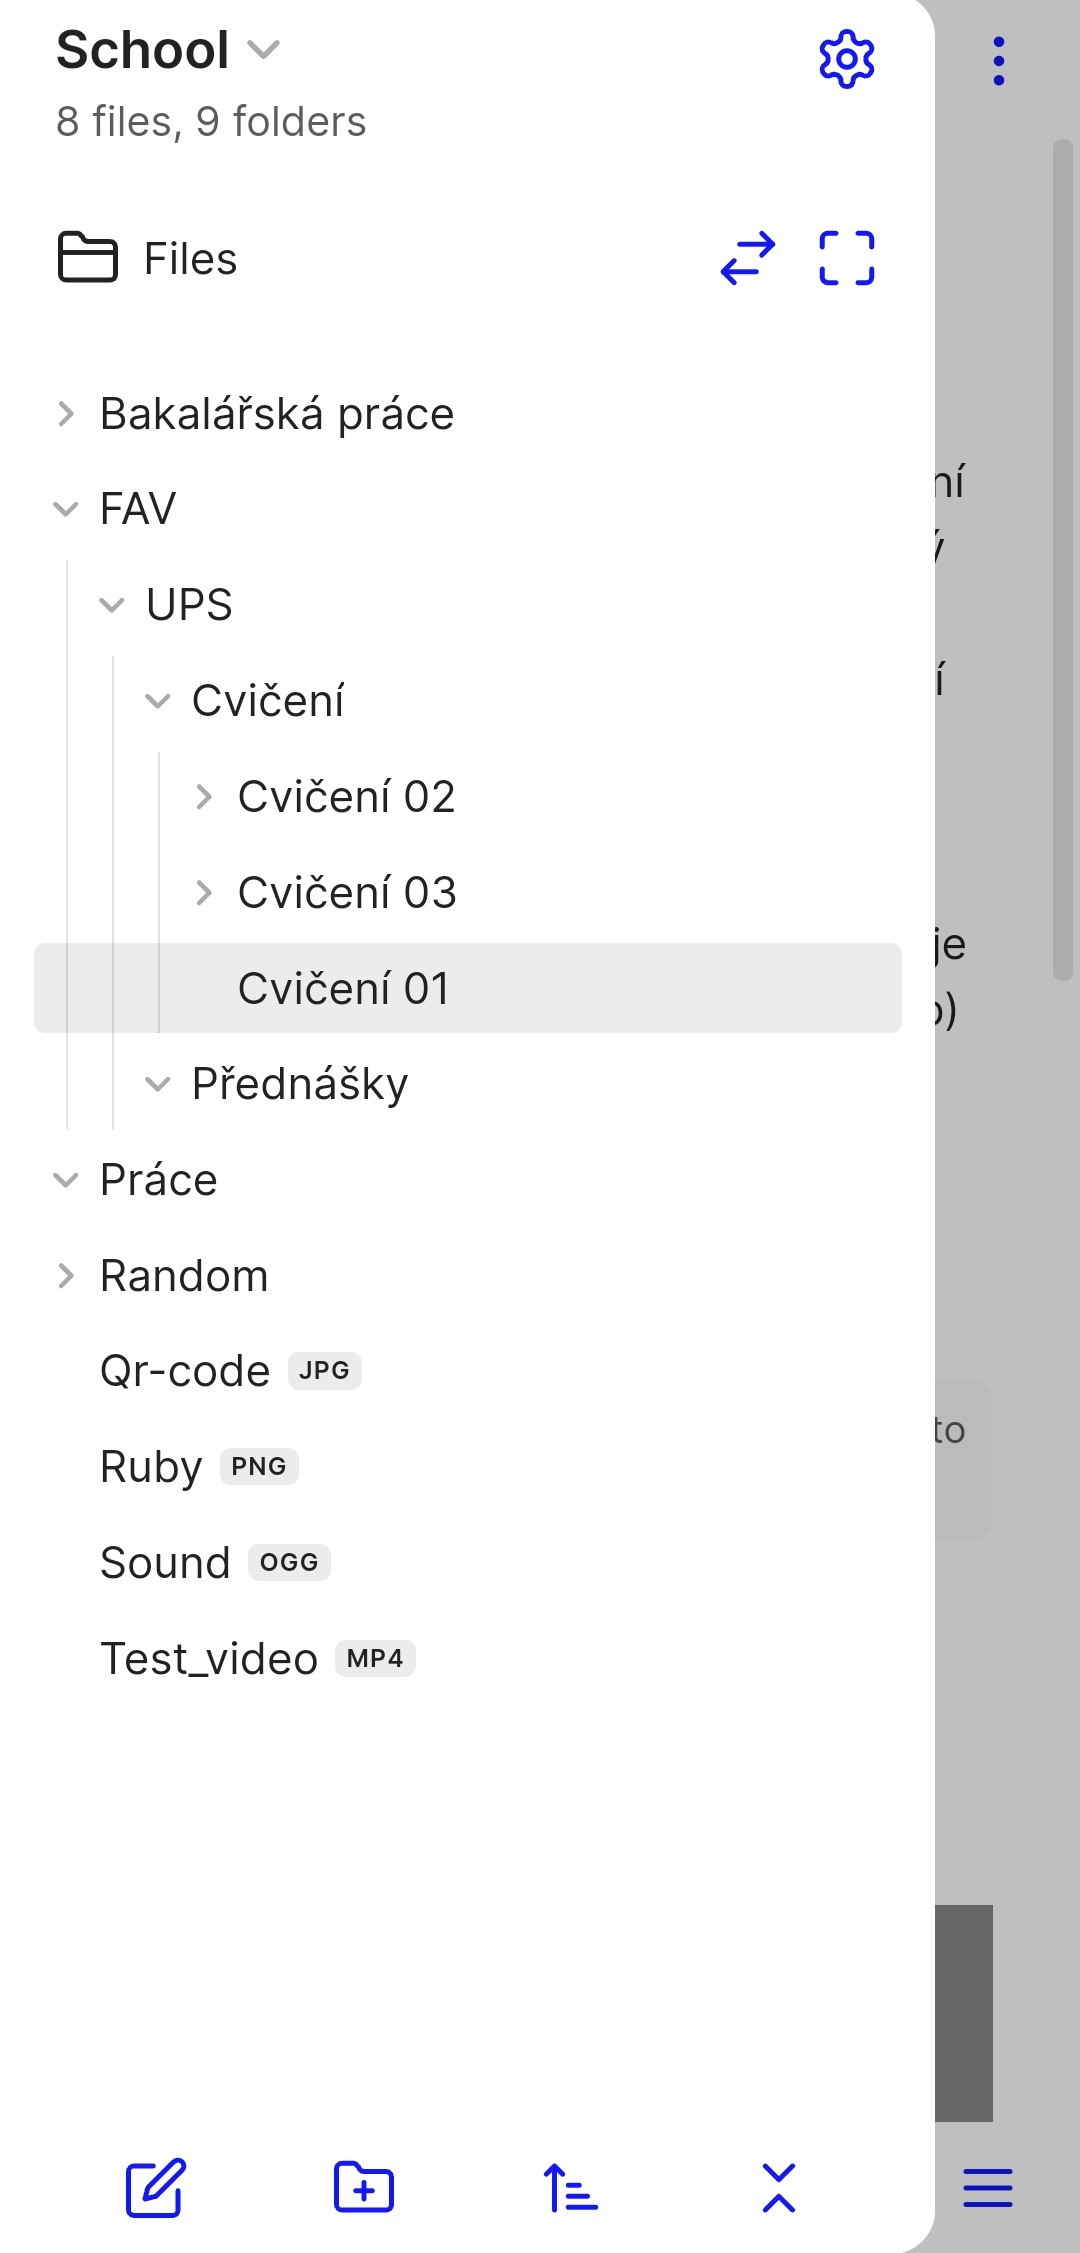
\includegraphics[width=0.3\textwidth]{img/BP-Runt/Obsidian/Obsidian_hierarchie.jpg}
  \caption{Hierarchie v mobilní aplikaci Obsidian}
  \label{fig:hierarchy_obsidian}
\end{figure}

Obsidian nabízí podobně jako ostatní testované aplikace funkce vyhledávání, filtrování, řazení a navíc ještě slučování více poznámek do jedné a organizaci do~bloků. Jedinečnou funkcí Obsidianu je graficky zobrazený graf, který zobrazuje závislosti mezi poznámkami. Uživatel si tak může vytvořit vlastní sémantickou síť nebo myšlenkovou mapu. Pro rozšíření základní funkcionality a vyladění pracovního prostředí podle svého vkusu, mají uživatelé možnost si vybrat některé z tisíce rozšíření. Pokud by uživatel nenašel vhodný vzhled nebo rozšíření, které potřebuje, má možnost se podívat do dokumentace \gls{API}, ve které je podrobně popsáno, jak si vytvořit vlastní rozšíření nebo upravit vzhled aplikace.

\section{Srovnání vybraných aplikací}

V rámci analýzy byl prozkoumán trh s aplikacemi pro tvorbu poznámek. Bylo vyzkoušeno a otestováno pět z nich. Jak již bylo řečeno v úvodu, na trhu existuje opravdu spoustu aplikací, které se zaměřují na tvorbu poznámek. K dalším aplikacím patří například Google Keep, která umožňuje vytváření poznámkových lístečků. Dále můžeme zmínit poznámkové aplikace Apple's Notes, Ulysses a Bear vytvořené primárně pro zařízení společnosti Apple a aplikace Confluence, Slite a Coda určené především pro dokumentaci a kooperaci ve firemním prostředí.

Při zkoušení jednotlivých aplikací jsme si mohli všimnout jejich odlišností, pozitiv, negativ a speciálních funkcí. Jednou z odlišností byla dostupnost na platformách. Z vybraných aplikací byly všechny dostupné na Android a poznámky se daly zobrazit a upravit i~na počítači. Přehled o dostupnosti na platformách je uveden v~tabulce~\ref{tab:tableOfPlatforms}. 

\begin{table}[h]
    \centering
    \caption{Tabulka dostupnosti aplikací na platformách}
    \begin{tabularx}{\textwidth}{|X|Y|Y|Y|Y|Y|Y|}
        \hline
                & Android & iOS & Windows & Linux & macOS & Web \\
        \hline
        Evernote & \greencheck  & \greencheck  &  \greencheck  & \greencheck   & \greencheck   & \greencheck\\
        OneNote  & \greencheck     & \greencheck    & \greencheck     & \redxcheck   & \greencheck   & \greencheck \\
        Joplin  & \greencheck     & \greencheck    & \greencheck     & \greencheck   & \greencheck   & \redxcheck \\
        Notion  & \greencheck   & \greencheck    & \greencheck     & \redxcheck   & \greencheck   & \greencheck \\
        Obsidian  & \greencheck     & \greencheck    & \greencheck     & \greencheck   & \greencheck   & \redxcheck \\\hline
        
    \end{tabularx}
    \label{tab:tableOfPlatforms}
\end{table}

Z pohledu finanční strategie jsme si mohli všimnout dvou modelů. Některé aplikace využívaly freemium marketingového plánu, ve kterém je základní verze aplikace s omezenou funkcionalitou zdarma a další balíčky s více funkcemi se musí měsíčně platit. Další aplikace naopak preferovaly strategie bezplatné aplikace, kde jsou placené jen některé služby nebo velikost úložiště, bez kterého se v některých případech lze bez problémů obejít. 

Z hlediska organizace jsme si mohli všimnout štítků, shlukování do skupin, tvoření zkratek a hierarchické struktury. Hierarchie byla rovněž implementována různými způsoby. V některých případech jsme se setkali s omezenou hloubkou, kde každý typ souboru měl stanovenou úroveň, ve které se může nacházet, což může být celkem omezující. Jiné aplikace naopak umožňovaly hloubku neomezenou. Typy souborů, které se objevují v hierarchii, byly též velmi různorodé. Hierarchie byla nejčastěji zobrazena stromovou strukturou a seznamem. V některých případech jsme se setkali se spojením poznámek pomocí odkazů. Přesouvání je nejčastěji implementováno přesouváním drag-and-drop nebo zvolením cesty ze seznamu.

Další odlišnosti aplikací bylo uložení uživatelských dat a přístup k datům dat bez připojení k internetu. Pro synchronizaci bývá využito buď cloudového úložiště nebo serveru. Při sdílení dat mezi více uživateli, může vlastník nastavit práva dalším uživatelům. Data jsou nejčastěji šifrována algoritmem \gls{AES}-256. Zabezpečení dat při přesunu bylo často implementováno koncovým šifrováním. Ve větších společnostech se ve většině případů využívá kombinace moderních standardů \gls{TLS}, \gls{HTTPS}, \gls{HSTS} a \gls{SSL}.  
Funkcionalita aplikací bývá také velice odlišná. Některé aplikace nabízí pouze základní funkce s možností instalace některých rozšíření. Další mají v~základní verzi nespočet funkcionalit, ze kterých běžný uživatel využije jen malé procento. Srovnání nabízených funkcí je uvedeno v tabulce \ref{tab:mytableOfFunctions}
  

\begin{table}[h]
    \centering
    \caption{Shrnutí funkcí jednotlivých aplikací}
    \begin{tabular}{|>{\arraybackslash}p{3.5cm}|*{6}{>{\centering\arraybackslash}p{1.4cm}|}}
        \hline
                & Evernote & OneNote & Joplin & Notion & Obsidian \\
        \hline
        Synchronizace & \greencheck & \greencheck  &  \greencheck  & \greencheck & \yellowdollar    \\
        Sdílení poznámek & \greencheck & \greencheck  &  \yellowdollar  & \greencheck & \yellowdollar    \\
        Offline přístup  & \yellowdollar     & \greencheck &  \greencheck  & \redxcheck   & \greencheck   \\
         Ukládání verzí  & \greencheck   & \greencheck    & \greencheck     & \greencheck   & \yellowdollar    \\
        Úložný prostor  & 60~MB\footnotemark  & 5~GB    & $\infty$\footnotemark     & $\infty$   & $\infty$   \\
         Max počet úrovní  & 3  & 3    &  $\infty$  &  $\infty$  & $\infty$  \\
        \hline
    \end{tabular}
    \label{tab:mytableOfFunctions}
\end{table}

\footnotetext[8]{Maximální velikost nahraných dat za měsíc}
\footnotetext[9]{Omezeno fyzickými parametry zařízení}

\section{Shrnutí}

Zjistili jsme, jak vypadají a fungují vybrané aplikace pro tvorbu poznámek. Z~hlediska vývoje naší aplikace je vhodné se inspirovat dobře navrženými funkcemi a~zároveň se vyhnout nedostatkům, které by mohli by uživatele limitovat. Vyvíjená aplikace bude nabízet vytváření poznámek s neomezenou\footnote{Počet úrovní bude limitován fyzickými parametry zařízení.} úrovní zanoření, aby bylo například umožněno organizování výpisků z přednášek dle ročníku, předmětu, a rozlišovat mezi přednáškami a cvičeními. Aplikace bude také umožňovat synchronizaci poznámky mezi různými zařízeními. Poznámky by mělo, být možné synchronizovat i mezi počítačem a mobilním zařízením. Je důležité, aby byla aplikace bezplatná a jednoduše rozšířitelná. V kapitole \ref{chapter:navrh} tyto nápady zohledníme a~provedeme detailnější návrh specifikace aplikace. 

% _____________________________________________________________________________
%
%
%        CHAPTER Technologies
%
% _____________________________________________________________________________
%
\chapter{Technologie pro vývoj mobilních aplikací}

V této kapitole se podíváme na technologická řešení a nástroje, které lze využít pro tvorbu mobilních aplikací. Prozkoumáme různé přístupy vývoje a jejich prostředky. Vyhodnotíme vlastnosti, přednosti a omezení každé technologie. Na závěr kapitoly vybereme technologii, která bude využita pro tvorbu naší aplikace.

\section{Vývoj mobilních aplikací}

Existuje více způsobů vývoje mobilních aplikací. V základu můžeme typy vývoje rozdělit na nativní a multiplatformní vývoj. Multiplatformní vývoj pak můžeme dále rozdělit na nativní multiplatformní, hybridní a \gls{PWA}. Hlavním rozdílem mezi nativním a multiplatformním vývojem je cílení aplikace na jednu konkrétní platformu s čímž se pojí vyšší optimalizace u nativních aplikací. Multiplatformní vývoj má obvykle jeden zdrojový kód pro více platforem, což zkracuje dobu vývoje a snižuje náklady aplikací vyvíjených pro více platforem. \cite{Difference-native-non-native}

\section{Nativní vývoj} \label{native_development}
Nativní vývoj představuje proces, při kterém vývojáři vyvíjejí aplikace pro konkrétní platformu nebo zařízení. Pokud tedy budeme vyvíjet aplikaci pro Android a iOS, budeme muset vytvořit dvě samostatné verze aplikace. Výhodou nativního vývoje je~možnost plně využít funkcí, možností a předností daného operačního systému. To~vede k~lepšímu výkonu, optimalizaci, bezpečnosti, plnému přístupu k~hardwarovým funkcím (\gls{GPS}, fotoaparátu, mikrofonu a další), typickému vzhledu a~chování pro~daný operační systém. Nevýhodou je již zmíněný vývoj pouze na jednu platformu a s tím spojený delší čas vývoje, náklady a nutnost znát více technologií. Nativní vývoj se upřednostňuje zejména u aplikací, ve kterých je důležitý vysoký výkon, časté využívání hardwarových funkcí a pokročilé interakce s~uživatelem. \cite{native_apps} \cite{native-vs-multiplatform}

\vspace{0.5cm}

Pro vývoj aplikací pro platformy iOS se nejčastěji používají programovací jazyky Objective-C a Swift, společně s využitím vývojového prostředí Xcode. Na~rozdíl od~platformy Android, má operační systém iOS neveřejný zdrojový kód, vytvořený výhradně pro hardware společnosti Apple. Pro vývoj pro platformu iOS je~tedy nezbytné použití zařízení Mac. Po dokončení vývoje lze aplikaci distribuovat prostřednictvím obchodu App Store. \cite{raygun-native-development}

Aplikace pro platformu Android se nejčastěji vyvíjí v jazycích Java a Kotlin, přičemž od roku 2017 je Kotlin společností Google označen jako oficiální jazyk pro vývoj aplikací na platformu Android\footnote{https://blog.jetbrains.com/kotlin/2017/05/kotlin-on-android-now-official/}. Pro vývoj je doporučováno používat Android Studio. Používání tohoto vývojového prostředí není povinné, avšak v nabídce je~široká škála funkcionalit zahrnující návrh uživatelského rozhraní, kompilaci zdrojového kódu a v neposlední řadě emulátory mobilních zařízení, které dokážou vývojářům značně zjednodušit vývoj. Aplikace je možno vydávat v obchodě Google Play, odkud si ji mohou stáhnout nebo zakoupit ostatní uživatelé. \cite{Michal_Zopp} \cite{raygun-native-development}


\subsection{Kotlin}

Kotlin je open-source\footnote{https://github.com/JetBrains/kotlin} programovací jazyk, vyvinutý společností JetBrains. Jedná se~o~staticky typovaný a objektově orientovaný programovací jazyk, který je spustitelný na \gls{JVM}, s plnou podporou knihovních tříd Java a~platformou Android. Původně byl Kotlin navržen s cílem poskytnout vývojářům jednodušší a stručnější syntaxi ve srovnání s jazykem Java. V současné době je Kotlin určený především pro vývoj mobilních aplikací. Díky své univerzálnosti lze však Kotlin použít též k vytváření serverů, webových stránek nebo aplikací pro datové analýzy. \cite{kotlin-docs} \cite{techtarget-kotlin}

Oproti jazyku Java představuje Kotlin mladší programovací jazyk, který nabízí moderní funkce, stručnou a čitelnou syntaxi. Kotlin zavádí koncept takzvaných datových tříd, které jsou primárně určeny k uchovávání dat. S použitím této deklarace jsou třídy automaticky vybaveny metodami \texttt{equals()}, \texttt{hashCode()}, \texttt{toString()} a \texttt{copy()}. Gettery a settery jsou nahrazeny přístupem k~vlastnosti viz zdrojový kód \ref{kotlin_class}.

\begin{code}{Java}{Definování třídy v jazyce Kotlin \label{kotlin_class}}
data class MyClass(private var myField: Int) {
   fun getMyField() = myField
   fun setMyField(value: Int) { myField = value }
}
\end{code}

V Kotlinu rozlišujeme dva hlavní typy proměnných \texttt{val} a \texttt{var}, kterým nemusíme explicitně zadávat datový typ. Tyto proměnné se liší dle toho, zda lze hodnotu po nadefinování změnit. Proměnná \texttt{val} definuje hodnotu, která nemůže být změněna, zatímco \texttt{var} definuje proměnnou, jejíž hodnota může být při běhu programu změněna. Kotlin při definici proměnné nabízí funkci „Null safety“, která má za cíl zabránit chybě \texttt{NullPointerException}, která je častým problémem při vývoji Java aplikací. Vývojáři mohou touto funkcí explicitně deklarovat, zda proměnná může obsahovat hodnotu \texttt{null}, pomocí znaménka otazníku viz zdrojový kód \ref{kotlin_val_var}.

\begin{code}{Java}{Proměnné v jazyce Kotlin \label{kotlin_val_var}}
val title = "Kotlin" // Proměnnou po definování nelze změnit
var title = "Kotlin" // Proměnná, kterou lze v průběhu změnit
var title: Any = "Kotlin" // Proměnná může být libovolný datový typ
var name: String = "Kotlin" // Proměnná nemůže být null
var name: String? = null // Proměnná může být null
\end{code}

Dalším významným rozdílem oproti Javě je podpora funkcionálního programování. Kotlin podporuje lambda výrazy, funkce vyššího řádu a rozšiřující funkce viz zdrojový kód \ref{kotlin_functional}. Kotlin rovněž podporuje korutiny, které poskytují jednodušší realizaci asynchronního programování oproti složitější práci s vlákny v Javě. Kotlin nevyžaduje ošetření výjimek, zpracovává primitivní typy jako objekty, dále můžeme najít mnoho dalších vylepšení oproti Javě. \cite{moskala2017android} \cite{jemerov2017kotlin} \cite{kotlin-vs-java}

\begin{code}{Java}{Funkcionální programování v jazyce Kotlin \label{kotlin_functional}}
// Lambda výrazy
val list = listOf(1, 2, 3)
// Zdvojnásobení každého prvku v seznamu
val doubledList = list.map { it * 2 }

// Funkce vyššího řádu, která přijíma dva celočíselné argumenty a jednu funkci
fun higherOrderFunc(x: Int, y: Int, f: (Int, Int) -> Int): Int {
    return f(x, y)
}
// Provedení sečtení dvou čísel
val result = higherOrderFunc(3, 4) { x, y -> x + y }

// Rozšiřující funkce umožňuje existující třídy bez nutnosti dědění
fun Int.isEven() = this \% 2 == 0
val isFourEven = 4.isEven()
\end{code}

\section{Nativní multiplatformní vývoj} \label{Cross_platform_development}

Multiplatformní vývoj využívá technologie, ve kterých lze napsat část nebo dokonce celý kód pro více platforem. Tento kód je následně zkompilován do nativní verze kódu pro různé platformy. V tomto aspektu se odlišují od hybridních aplikací. Vzhledem k tomu, že se využívá nativního vykreslování, je optimalizace srovnatelná s~nativním vývojem. Výkon však záleží na frameworku, který se vývojář rozhodne použít. Mezi populární nativní multiplatformní frameworky patří React Native, Flutter a .NET MAUI. \cite{Difference-native-non-native} \cite{multiplatform-apps-yojji}

\subsection{React Native} \label{React_native}

React native je open-source framework umožňující vyvíjet mobilní aplikace s použitím JavaScriptu a Reactu. Tento framework vznikl v létě 2013 jako interní projekt společnosti Facebook v rámci hackathlonu. V březnu 2015 pak společnost Facebook zveřejnila zdrojový kód na platformě GitHub\footnote{https://github.com/facebook/react-native} \cite{brainhub-react-native}. React Native obsahuje předdefinovanou sadu komponent, jako jsou například View, Text nebo Image, které se~přímo mapují na nativní komponenty platformy. Tyto komponenty lze též kombinovat a~sestavovat tak komplexnější komponenty, které lze použít v aplikaci. \cite{react-native} \cite{what-is-react-native}

\begin{figure}[h!]
  \centering
  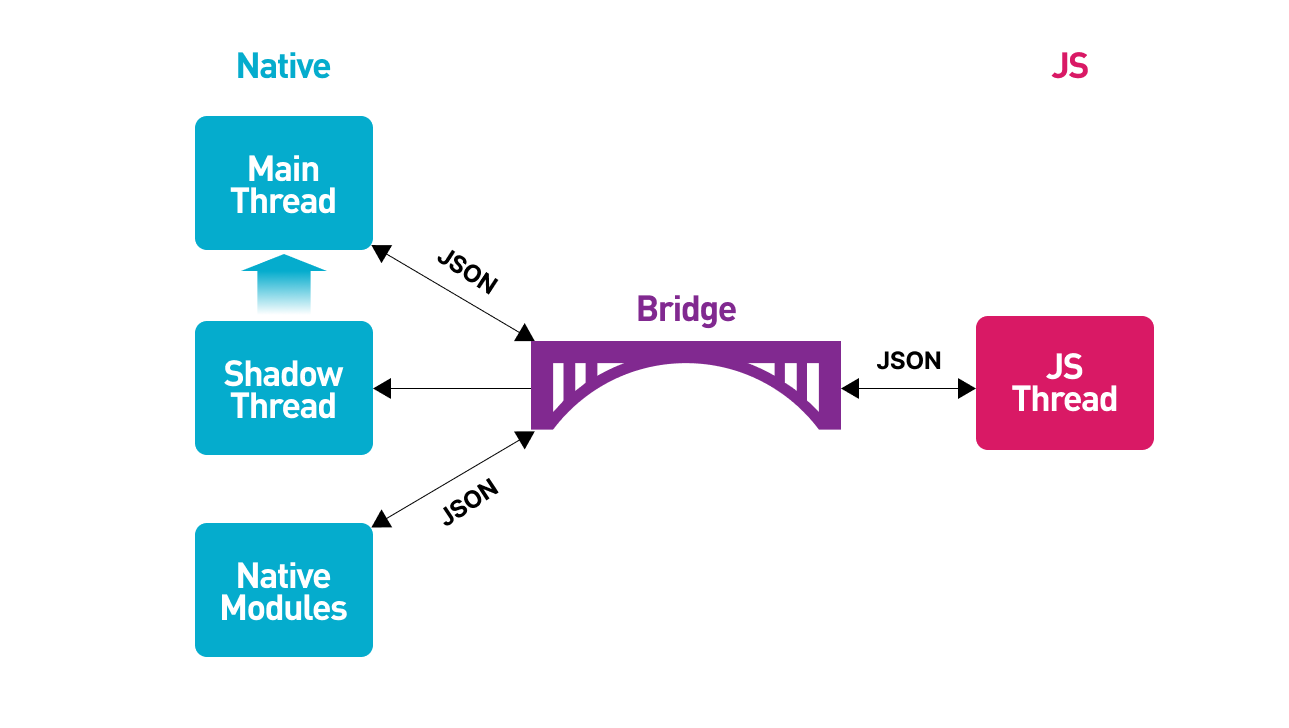
\includegraphics[width=0.95\textwidth]{img/BP-Runt/Technologies/react_native_bridge_threads.png}
  \caption{Architektura bridge v React Native \cite{react-bridge-figure}}
  \label{fig:react_bridge}
\end{figure}

React Native se na rozdíl od hybridních framewoků nespoléhá na webové zobrazení (WebView), ale na skutečné komponenty a přístup k \gls{API} poskytnutý nativními platformami. Z počátku React Native používal koncept „mostu", který umožňoval asynchronní komunikaci mezi prvky JavaScriptu a nativními prvky viz obr. \ref{fig:react_bridge}. Logika mostu je zde stejná jako v případě webových aplikací, kdy o sobě vrstvy frontendu a backendu nemusí nic vědět, ale musí spolu umět komunikovat. Pro~vzájemnou komunikaci se používá zpráv ve~formátu \gls{JSON}. Samotný React Native závisí na čtyřech vláknech:

\begin{itemize}
    \itemsep0em 
    \item \textbf{Hlavní vlákno:} jedná se o vlákno, ve kterém je spuštěna aplikace. Toto vlákno je zodpovědné za interakci s uživatelem a vykreslování uživatelského rozhraní,
    \item \textbf{JavaScriptové vlákno:} je zodpovědné za provádění logiky aplikace,
    \item \textbf{Stínové vlákno:} je vlákno, které je spuštěné společně s JavaScript vláknem. Jeho úkolem je vypočítat pozice rozvržení (View) a zkonstruovat strom komponent (Layer), 
    \item \textbf{Vlákno nativních modulů:} stará se o přístup k \gls{API} dané platformy.
\end{itemize}

Od verze 0.68 je možné používat novou architekturu React Native, která upouští od mechanismu mostu ve prospěch JavaScriptového rozhraní. \gls{JSI} je odlehčená univerzální vrstva, která může navázat přímé spojení s nativními rozhraními \gls{API} viz obr. \ref{fig:react_JSI}. To umožňuje synchronní komunikaci mezi JavaScriptem a nativními prvky, což vede ke zvýšení výkonu. \cite{what-is-react-native} \cite{medium-how-react-works}

\begin{figure}[h!]
  \centering
  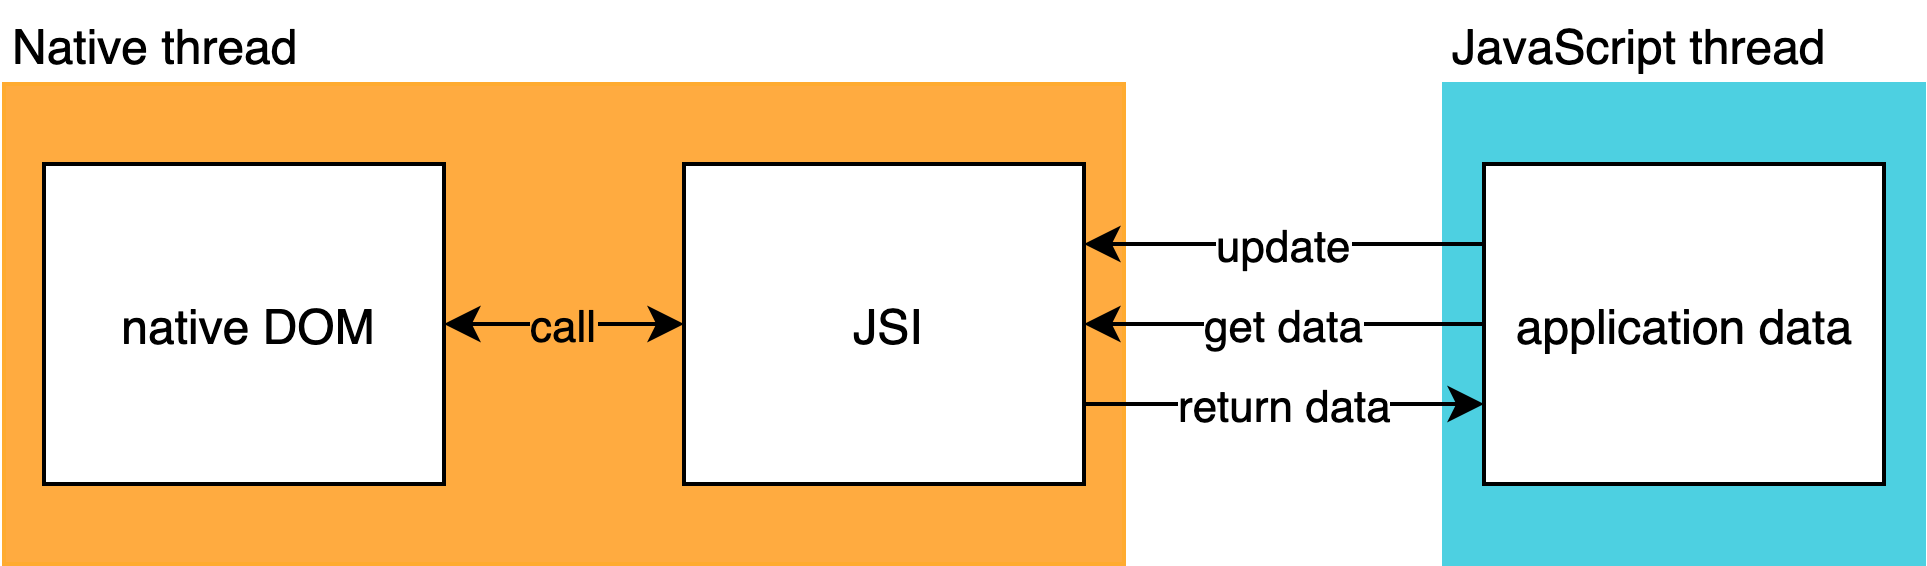
\includegraphics[width=0.85\textwidth]{img/BP-Runt/Technologies/react-JSI.png}
  \caption{Architektura \gls{JSI} v React Native \cite{react-bridge-figure}}
  \label{fig:react_JSI}
\end{figure}


\noindent Framework React Native nabízí některé výhody, mezi které například patří:

\begin{itemize}
    \item \textbf{Společný kód:} Využití stejné kódové základny pro různé platformy urychluje vývoj, zkracuje dobu uvedení na trh a usnadňuje údržbu. Stejný kód lze využít pro webové a mobilní aplikace, pokud používají React Native,
    \item \textbf{Rozsáhlá komunita:} React Native má rozsáhlou aktivní komunitou vývojářů. Díky této komunitě existuje velké množství knihoven, nástrojů, komponent a návodů. Rozsáhlá komunita může zrychlit řešení problému, protože je~vyšší šance, že někdo narazil na stejný problém,
    \item \textbf{Výkon:} V porovnání s Hybridními aplikacemi poskytuje React Native výkon podobný nativnímu,
    \item \textbf{Aktualizace:} React Native je populární framework, který dostává pravidelné aktualizace a vylepšení, které společnost Facebook vydává, 
    \item \textbf{Jazyk:} Při implementaci se používají populární jazyky JavaScript a TypeScript, které se používají i u webových aplikací,
    \item \textbf{Hot Reloading:} Tato funkce umožňuje vývojářům vidět provedené změny bez nutnosti znovu kompilovat kód.  \cite{what-is-react-native}
\end{itemize}

\noindent Mezi nevýhody React Native naopak patří:

\begin{itemize}
    \item \textbf{Mladá technologie:} Jedná se o relativně mladou technologii, která má jistá omezení, chyby a problémy, které je třeba vyřešit. Některé moduly ve framewokru neexistují, což znamená, že vývojáři mohou potřebovat více času na vytvoření vlastních modulů, 
    \item \textbf{Animace a interakce:} React Native není přizpůsobený na vytváření komplexních animací a interakci se složitými gesty, důvodem je JavaScriptová část aplikace, 
    \item \textbf{Výkonnost:} Přestože je výkon React Native lepší než u~hybridních aplikací, stále je zde rozdíl mezi nativním řešením.
\end{itemize}

Co se týče komponent, má vývojář na výběr z oficiálních komponent, které jsou uvedeny v dokumentaci React Native\footnote{https://reactnative.dev/docs/components-and-apis}, nebo využít jedné z mnoha komunitních knihoven, díky rozsáhlé komunitě, kterou React Native má. Poslední možností je~vytvořit si vlastní komponenty. 

\subsection{Flutter} \label{Flutter}

Flutter je open-source technologie společnosti Google pro vytváření mobilních, desktopových a webových aplikací. Jedná se o celkem mladou technologii, který byl oficiálně jako projekt spuštěn v roce 2017 a následně v prosinci 2018 byla zveřejněna první stabilní verze. Pomocí Flutteru je vytvořeno mnoho známých aplikací. Jedná se například o eBay, Alibaba.com, Google Classroom a Google Pay. \cite{Flutter} \cite{Bartosińska_Dembny_2024}

Flutter není programovací jazyk, framework ani knihovna, ale kompletní \gls{SDK} obsahující vykreslovací jádro, widgety, testovací a integrační \gls{API} a mnohé další viz obr. \ref{fig:flutter_architecture}. Toto \gls{SDK} je tvořeno třemi hlavními částmi: \cite{AltexSoft_2022} \cite{Bartosińska_Dembny_2024}

\begin{itemize}
    \item \textbf{Embedder} používá jazyk specifický pro danou platfromu a zajišťuje bezproblémový běh aplikace na různých operačních systémech, 
    \item \textbf{Engine}, napsaný v C/C++, poskytuje nízkoúrovňovou implementaci základních rozhraní \gls{API} aplikace Flutter, které se stará o vykreslování vizuálních prvků vždy, když se něco změní. Zároveň také zajišťuje veškerou základní funkcionalitu, mezi kterou patří kompilace jazyku Dart, rozložení textu, systémové eventy, vstupy/výstupy a další, 
    \item \textbf{Framework} je založen na programovacím jazyku Dart. Jedná se o bohatou sadu knihoven a funkcí, které Flutter poskytuje vývojářům.
\end{itemize}

\begin{figure}[h!]
  \centering
  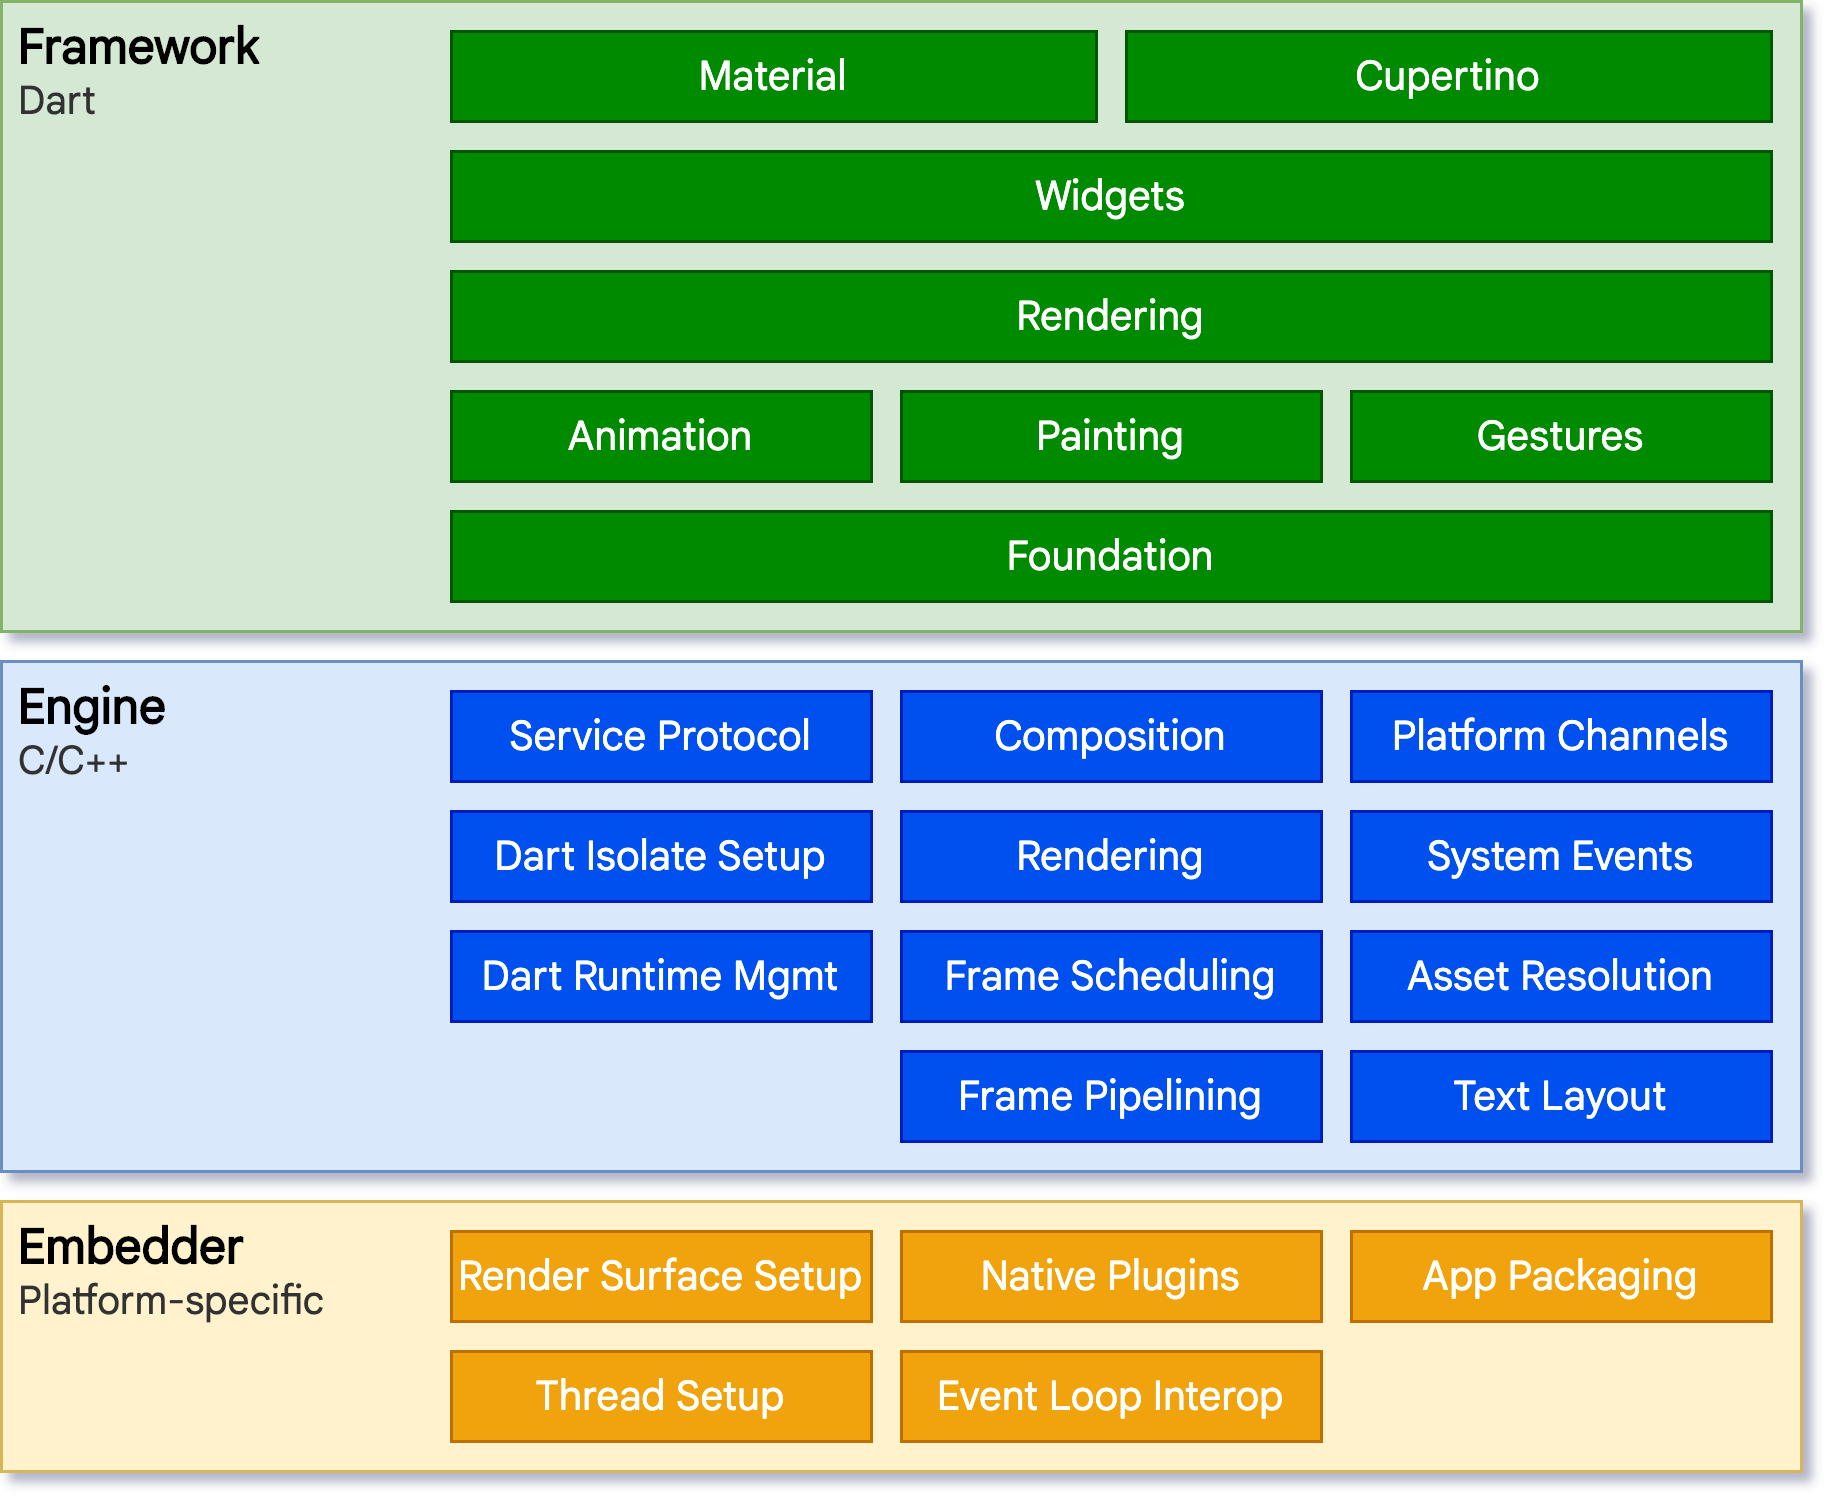
\includegraphics[width=0.9\textwidth]{img/BP-Runt/Technologies/flutter_archdiagram.png}
  \caption{Architektura technologie Flutter \cite{Flutter}} %https://docs.flutter.dev/resources/architectural-overview
  \label{fig:flutter_architecture}
\end{figure}

Pro vývoj aplikací se využívá jazyk Dart. Jedná se o objektově orientovaný jazyk, který svou syntaxí připomíná jazyk Java nebo C++. Na rozdíl od jiných frameworků (např. React Native) nepotřebuje Dart žádný mezilehlý krok k přeložení a propojení nativního zobrazení platformy. Dart podporuje dva způsoby kompilace \gls{AOT} a \gls{JIT}. \gls{AOT} kompiluje zdrojový kód do nativního před spuštěním aplikace. \gls{JIT} překládá zdrojový kód až v okamžiku, když je aplikace spuštěna, čehož se využívá hlavně při vývoji, kdy vývojář vidí změny které provádí. \cite{Bartosińska_Dembny_2024} \cite{AltexSoft_2022}

Ve Flutteru je vše složeno z widgetů. Jedná se o základními stavebními prvky uživatelského rozhraní, které se do sebe dají vkládat a tím tvořit složité widgety. Při vytváření uživatelského rozhraní se definuje strom widgetů viz obr. \ref{fig:flutter_widget_tree}, který popisuje, jak vypadá vzhled naší aplikace. Widgety kromě vzhledu aplikace také zohledňují její aktuální stav. Flutter zavádí dvě hlavní třídy widgetů, a to bezstavové (\texttt{Stateless}) a stavové (\texttt{Statefull}). Widgety, které nemění v průběhu své existence svůj stav (ikony, popisky, tlačítka a další) jsou definovány \texttt{Stateless} widgety. Pokud se vlastnosti a stav widgetu v průběhu běhu aplikace mění na základě interakce s uživatelem nebo jiných faktorů, jedná se o \texttt{Statefull} widget. Oba typy widgetů obsahují metodu pro překreslení build, která překresluje obsah při změně.

\begin{figure}[h!]
  \centering
  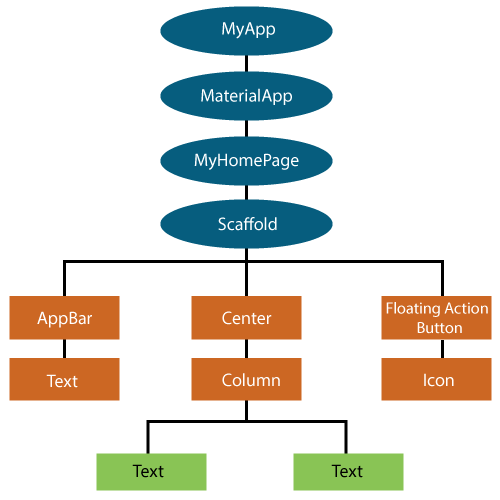
\includegraphics[width=0.75\textwidth]{img/BP-Runt/Technologies/flutter-widget-tree.png}
  \caption{Widget tree \cite{flutter-widget-tree}}
  \label{fig:flutter_widget_tree}
\end{figure}

\noindent Mezi výhody Flutteru patří: \cite{pros-and-cons-flutter} \cite{AltexSoft_2022}
\begin{itemize}
    \itemsep0em
    \item \textbf{Společný zdrojový kód:} Flutter je multiplatformní, umožňuje vytvářet aplikace pro více platforem zároveň. Flutter podporuje celkem sedm platforem: Android, iOS, Windows, Linux, macOS, web a Google Fuchsia (operační systém vyvíjený společností Google),
    \item \textbf{Rychlý vývoj uživatelského rozhraní:} Flutter poskytuje bohatou sadu komponent, které umožňují vytvářet přizpůsobitelná uživatelská rozhraní za krátkou dobu,
    \item \textbf{Stálá podpora:} Společnost Google garantuje dlouhodobou podporu technologie Flutter,
    \item \textbf{Vysoký výkon:} Flutter využívá přímé kompilace díky tomu je výkon Flutteru srovnatelný s nativními aplikacemi,
    \item \textbf{Hot reload:} Změny, které provede vývojář v kódu se ihned promítnou v~aplikaci, což vede ke zvýšení produktivity programování,
    \item \textbf{Snadná internacionalizace:} Flutter nativně podporuje widgety založené na knihovně intl\footnote{https://pub.dev/packages/intl}, která zjednodušuje proces internacionalizace. V současné době je podporováno 78 jazyků, různé měny, měrné jednotky, zobrazování textu zprava doleva a mnohá další specifika lokalizací,
     \item \textbf{Rychlé učení:} Naučit se jazyk Dart by neměl být velký problém vzhledem k rozsáhlé dokumentaci a stále rostoucí komunitě. Začínající programátor nemusí mít velké zkušenosti s programováním mobilních aplikací.
\end{itemize}

\noindent Mezi nevýhody Flutteru můžeme zařadit:
\begin{itemize}
    \item \textbf{Nedostatek knihoven třetích stran:} Pro Flutter je vytvořeno méně komunitních knihoven než je tomu třeba u React Native nebo jiných starších technologií,
    \item \textbf{Velikost aplikace:} Vzhledem k tomu, že má Flutter vestavěné widgety, minimální velikost aplikace přesahuje 4~MB, což je více než u nativních aplikací,
    \item \textbf{Rozšíření jazyku Dart:} Z hlediska popularity Dart zaostává například za~JavaScriptem, Javou nebo Kotlinem. Vývojáři, kteří se rozhodou vytvořit Flutter aplikaci jsou nuceni se naučit nový programovací jazyk, který s velkou pravděpodobností nepoužijí v žádné další technologii.
\end{itemize}

Při hledání vhodných komponent má vývojář možnost zkusit najít vhodné widgety v katalogu s widgety\footnote{https://docs.flutter.dev/ui/widgets}, kde lze najít například widgety Material design pro Android nebo Cupertino pro iOS. Pokud zde vývojář nenalezne widgety, které potřebuje, má možnost zkusit prohledat stránku pub.dev\footnote{https://pub.dev/}, což je oficiální stránka s~Flutter knihovnami. V případě, že ani zde není to, co vývojář potřebuje, lze ještě zkusit najít požadované knihovny na platformě GitHub, webové stránce Flutter Awesome a dalších online zdrojích.

\section{Hybridní vývoj} \label{hybrid_development}

Hybridní aplikace kombinují prvky webových aplikací s prvky nativních aplikací. Aplikace se vyvíjejí s využitím standardních webových technologií \gls{HTML}, \gls{CSS} a Javascriptu. Na rozdíl od webových aplikací, které fungují přímo ve webovém prohlížeči, se hybridní aplikace spouští jako nativní, využívající vlastní vestavěný prohlížeč WebView (Android) nebo WKWebView (iOS). Aplikace je také zabalena do nativního kontejneru viz obr. \ref{fig:hybrid_schema}, který umožňuje přistupovat k~funkcím daného operačního systému skrze pluginy.

\begin{figure}[htbp]
    \centering
    \includesvg[width=0.9\textwidth]{img/BP-Runt/Technologies/hybrid_app_schema.svg}
    \caption{Porovnání nativní, hybridní a webové aplikace (překresleno z \cite{hybrid-app-picture})}
    \label{fig:hybrid_schema}
\end{figure}

%predelany obrazek z https://www.upwork.com/resources/hybrid-app

Hybridní aplikace přinášejí výhodu jedné kódové základny, která snižuje náklady, údržbu a zaručuje stejnou funkcionalitu napříč zařízeními. Aby však aplikace efektivně komunikovala se systémovými \gls{API} a konzistentně fungovala na dané platformě, je často nutné napsat část nativního kódu. Tato implementace může vést k rozdílům v uživatelském rozhraní a ovládání aplikace na různých platformách. Hlavní nevýhodou hybridních aplikací je nižší výkon ve srovnání s nativními aplikacemi, jakožto důsledek závislosti na vestavěném prohlížeči. Mezi hybridní technologie se řadí Ionic a Apache Cordova. \cite{appflyer-hybrid-app} \cite{hybrid-mobile-app-development}

%https://www.techtarget.com/searchsoftwarequality/definition/hybrid-application-hybrid-app?vgnextfmt=print
% native shell se přizpůsobuje (stahuje) při stažení z obchodu s aplikacemi prostřednictvím prohlížeče, který je v aplikaci zabudován. Tento prohlížeč běží na back-endu a je pro uživatele neviditelný.
% překlad plugins?

\subsection{Ionic} \label{Ionic}

Ionic framework je open-source\footnote{Zdrojový kód Inonic zveřejněn zde: https://github.com/ionic-team/ionic-framework} sada nástrojů určená pro vývoj hybridních mobilních aplikací. První verze byla publikována v roce 2013 a byla postavena na technologiích Angular a Apache Cordova. V dnešní době tento framework poskytuje sadu webových komponent, které umožňují uživatelům vyvíjet aplikaci ve frameworku Angular, React nebo Vue.js. \cite{Ionic_framework}

Mezi výhody frameworku Ionic patří nezávislost na platformě a s tím spojený společný kód, bohatá nabídka komponent a pluginů, možnost vyvíjet v prohlížeči, dobře napsaná dokumentace a podpora komunity. Mezi nevýhody můžeme zařadit nižší výkon ve srovnání s nativními technologiemi a bezpečnostní problémy, musí se~řešit specifické bezpečnostní rizika všech platforem, které však lze řešit správnými bezpečnostními opatřeními. \cite{Pokorska_2022}

Ionic poskytuje velké množství optimalizovaných komponent navržených pro mobilní zařízení. Tyto komponenty mohou být dále přizpůsobeny pro každou platformu pomocí \texttt{Platform Styles}, ve kterých má každá platforma nastavený typický vzhled a chování. Pokud se pokusíme najít vhodné komponenty pro náš projekt, máme na výběr z velkého množství oficiálních komponent, které jsou uvedeny v dokumentaci\footnote{https://ionicframework.com/docs/components}. Stromová struktura bohužel v seznamu oficiálních komponent chybí, avšak v Ionic Market place\footnote{https://market.ionicframework.com}, ve kterém můžeme najít bezplatné i zpoplatněné šablony, motivy, komponenty a pluginy navržené pro vývoj Ionic aplikací, lze~najít několik implementací této struktury. Další možností pro hledání užitečných komponent a knihoven je například server GitHub, knihovny npmjs a další webové stránky jako syncfusion\footnote{https://www.syncfusion.com}, určené k nahrání komponent. 

%iom-menu = drawer, ion-accordion = rozbalovací seznam

\section{Progresivní webové aplikace} \label{progressive_web_app}

\gls{PWA} je typ webové aplikace, který může fungovat jako webová stránka i mobilní aplikace. Tyto aplikace se nedají považovat za plnohodnotné mobilní aplikace, neboť jde jen o obal webového prohlížeče, který tvoří technologie Service Workers a \gls{JSON} manifest:

\begin{itemize}
    \item \textbf{Service Workers:} jsou skripty, které umožňují práci s mezipamětí. To umožňuje uživatelům práci i bez připojení k internetu a současně přispívá k rychlejšímu běhu aplikace,
    \item \textbf{\gls{JSON} manifest:} Obsahuje základní informace, jako je název aplikace, použité ikony nebo barvy a zajišťuje přístup k hardware. Jeho cílem je zvýšit zážitek podobný nativní aplikaci.
\end{itemize}

\gls{PWA} se chovají a vypadají stejně jako běžné webové stránky, které poskytují responzivní design a~lze je vyhledat v internetovém prohlížeči. Navíc bývají rychlejší než klasické webové stránky, mají možnost fungovat i bez internetového připojení a lze je přidat na domovskou obrazovku přímo z prohlížeče. Stejně jako mobilní aplikace mohou být publikovány v obchodech s mobilními aplikacemi App Store a Google Play. Přestože \gls{PWA} mohou využívat hardwarové funkce, tento přístup nemusí být ke všem mobilním senzorům, aplikace nemusejí mít nativní vzhled a~v~případě iOS může nastat problém s instalací aplikace na domovskou obrazovku. Zdrojový kód je jednotný pro všechna zařízení, což výrazně usnadňuje a zrychluje vývoj pro~různé operační systémy. Příkladem \gls{PWA} je například Pinterest, Spotify, Uber, X (bývalý Twitter) nebo TikTok. \cite{progressive_web_apps} \cite{pwa-vue}

\section{Shrnutí}

V rámci kapitoly technologií pro vývoj mobilních aplikací jsme prozkoumali různé způsoby a technologie používané pro vytváření mobilních aplikací. S ohledem na~charakteristiky aplikace pro vytváření poznámek, je praktické, aby byla aplikace přístupná z více typů zařízení, umožňující uživatelům prohlížet a upravovat poznámky jak na mobilním zařízení, tak na počítači. Dále též v případě změny operačního systému z Android na iOS, je dobré, aby uživatelé mohli dále spravovat bez problémů své poznámky. Aplikace též nepotřebuje složité animace a velký výpočetní výkon. Z těchto důvodu jsem se rozhodl při vývoji využít nativní multiplatformní vývoj. 

Při rozhodování mezi nativními multiplatformními technologiemi jsem se rozhodl upřednostnit Flutter. Hlavními faktory mého rozhodnutí byla rostoucí popularita, což znamená vyšší použitelnost technologie v budoucnu, a vysoký výkon v porovnání s ostatními multiplatformními technologiemi. Flutter umožňuje kompilaci do nativního kódu, tím se eliminuje mezikrok komunikace s nativními komponentami. Další důvod rozhodnutí je technologie widgetů, která nabízí unikátní způsob, který vývojářům zjednodušuje vytváření uživatelského rozhraní.


% 00_____________________________________________________________________________
%
%
%        CHAPTER Ukládání dat
%
% _____________________________________________________________________________
%

\chapter{Ukládání dat} \label{chap:data}

V této kapitole se zaměříme na různé způsoby a technologie ukládání dat mobilních aplikací. Začátek kapitoly se zabývá ukládáním dat do lokálního úložiště mobilního zařízení. Další část kapitoly se věnuje technologiím, které lze využít pro synchronizaci dat. Tato část analyzuje nejdříve možnosti serverových a cloudových úložišť. V~závěru kapitoly jsou vybrány technologie, které budou použity při vývoji aplikace. % Data aplikací lze ukládat lokálně, pro běžnou práci s aplikací bez nutnosti připojení k internetu. Při ukládání online umožňujeme uživateli přístup k datům z více zařízení, možnosti synchronizace a sdílení s více uživateli. Tento přístup se~obvykle realizuje buď serverovým úložištěm nebo pomocí cloudových služeb. %Začátek kapitoly se zabývá ukládáním dat do lokálního úložiště zařízení. V další části se pak zabýváme ukládáním dat v serverových a cloudových úložištích. V závěru kapitoli vybereme technologie, které budou použity při vývoji aplikace.

\section{Lokální ukládání} 

Jedna z klíčových funkcionalit vytvářené aplikace je umožnění práce s daty bez~připojení k internetu. K dosažení této vlastnosti budeme muset ukládat uživatelská data do lokálního úložiště zařízení. Bez lokálního ukládání by všechna data po ukončení práce s aplikací zmizela a uživatel by se při opětovném spuštění aplikace setkal pouze s inicializačními daty. V následující části budou popsány možnosti lokálního ukládání dat na mobilním zařízení.

Ukládání dat aplikace na mobilním zařízení funguje rozdílně, než je tomu u~desktopových aplikací. Android poskytuje několik základních možností ukládání:
 

\begin{itemize}
    \item \textbf{Vnitřní úložiště:} Soubory, které se ukládají do soukromého adresáře aplikace. Tato data jsou určena pro použití konkrétní aplikací a jsou smazána společně s odinstalováním aplikace,
    \item \textbf{Externí úložiště:} Uložení dat do veřejné části paměti. Může se jednat o \gls{SD} kartu i pevně zabudovanou paměť v zařízení. Typicky to jsou fotky, videa, zvukové nahrávky a dokumenty, které byly vytvořeny v aplikaci,
    \item \textbf{Shared preferences:} Uložení soukromých dat základních primitivních typů ve formě klíč-hodnota,
    \item \textbf{Databáze:} Uložení dat do databáze s pomocí některé z knihoven (např. SQLite, Hive, Isar Database). \cite{android-storage} \cite{mistrostvi_android}
\end{itemize}

V další části se podíváme na použitelné knihovny pro ukládání lokálních dat ve~Flutter aplikacích.

\subsection{SharedPreferences}\label{Shared_preferences} 

SharedPreferences je nejjednodušší forma ukládání pro ukládání jednoduchých dat aplikace. Tato třída umožňuje ukládání malého množství jednoduše strukturovaných dat ve formě perzistentní mapy s páry klíč-hodnota. Pro Flutter je vytvořena knihovna \texttt{shared\_preferences}, která obaluje úložiště specifické pro konkrétní platformy (např. SharedPreferences pro Android, NSUserDefaults pro iOS a macOS). Knihovna je kompletně napsána v~jazyku Dart a je kompatibilní s platformami Android, iOS, Linux, macOS, Windows a~webovými aplikacemi. Podporované datové typy jsou \texttt{int}, \texttt{double}, \texttt{bool}, \texttt{String} a \texttt{List<String>}. \cite{mistrostvi_android} \cite{Shared_preferences_package}

\subsection{SQLite}\label{SQLite}

SQLite je malý a rychlý \gls{SQL} databázový engine, který je napsán v jazyce C. Jedná se o nejčastěji používanou relační databázi na světě, která je integrována do mobilních zařízení, počítačů a mnoha běžně používaných aplikací. Kompletní \gls{SQL} databáze má podporu funkcionalit klasických databázových serverů, jako je podpora více tabulek, indexování, podpora triggerů a vytváření pohledů. Veškerá data této databáze jsou uložena v jednom souboru. Pro Flutter je vytvořena knihovna \texttt{sqflite}\footnote{https://pub.dev/packages/sqflite}, která je kompletně přepsána do jazyka Dart. \cite{SQLite} \cite{mistrostvi_android} 

\subsection{Hive}\label{Hive}

Hive je rychlá a nenáročná NoSQL databáze ukládající data ve formátu klíč-hodnota, která je kompletně napsána v jazyce Dart. Tato databáze ukládá data s možností zabezpečení dat šifrovacím algoritmem \gls{AES}-256. \cite{Hive_package}

Všechna data, uložena knihovnou Hive, jsou organizována do boxů, což je obdoba tabulky v \gls{SQL}. Aplikace může mít libovolný počet boxů. Před použitím se~musí box otevřít. Při otevření klasického boxu se načtou všechna data z lokálního úložiště do paměti pro okamžitý přístup. Pokud máme aplikaci, která uchovává větší množství dat, lze využít líného načítání dat, které si zapamatuje jen všechny klíče a~adresy, kde jsou data jednotlivých klíčů uložena. Boxy mají operace pro zapisování, čtení a mazání dat (viz zdrojový kód \ref{hive_operations}).  \cite{Hive_documentation}

\begin{code}{Java}{Operace s Hive boxy\label{hive_operations}}
T value = box.get('key');   // Čtení dat
box.put('key', 'value');    // Ukládání dat
box.delete('key');          // Mazání dat
\end{code}

Hive podporuje kromě primitivních a složených datových typů (String, DateTime, List, Map) také objekty vytvořené uživatelem. V případě uživatelem vytvořených objektů je potřeba registrovat \texttt{TypeAdapter}, který převede objekt do binární podoby. Type adapter lze automaticky vygenerovat, pokud v definici našeho objektu doplníme anotace \texttt{@HiveType} na začátku třídy a \texttt{@HiveField}, které doplníme k~atributům třídy. Automatické vygenerování adaptéru pak provedeme příslušným příkazem.

\section{Serverové úložiště} \label{server_storing}

Na serverech lze vytvářet databáze, ve kterých se mohou uchovávat data. Při vytváření serveru lze zvolit mezi pořízením vlastního serveru nebo využitím služeb hostování serverů od externích poskytovatelů. Vytvoření vlastního serveru dává úplnou kontrolu nad aktualizacemi, zálohováním, zabezpečením citlivých dat a mnohými dalšími aspekty. To znamená, že se server může plně přizpůsobit požadavkům aplikace. Při vytváření serverové databáze je na výběr mezi relační (\gls{SQL}) a \gls{NoSQL} databází. \cite{in-house-servers}

\begin{figure}[h]
  \centering
  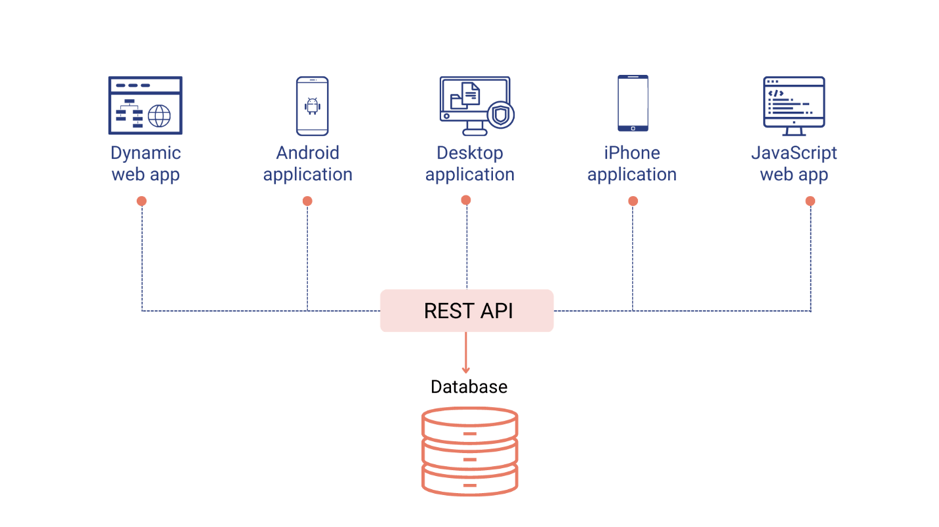
\includegraphics[width=0.95\textwidth]{img/BP-Runt/Data_storing/server/Understanding-REST-API.png}
  \caption{Princip fungování REST API \cite{understanding-rest-api}}
  \label{fig:restful-api}
\end{figure}

Při vývoji serverové části je vhodné vytvořit takzvané \gls{REST} \gls{API}, což je architektonický styl, který usnadňuje komunikaci mezi klientem a serverem viz obr. \ref{fig:restful-api}. \gls{REST} \gls{API} funguje jako propojení mezi databází a klientem, přičemž jsou obě strany na sobě navzájem nezávislé a komunikace je~bezstavová, tedy server se nezajímá o stav klienta. Komunikace využívá efektivní výměny dat pomocí definovaných \gls{URL} adres a \gls{HTTP} metod (GET, POST, PUT a DELETE). Mezi nejpoužívanější technologie pro psaní \gls{REST} \gls{API} patří Node.js, framework Java Spring Boot, Go a Ruby. \cite{codecami-rest} \cite{understanding-rest-api} \cite{rest-for-mobile-apps}

\subsection{Relační databáze} \label{lab:relational-database}

Relační databáze jsou systémy ukládání dat, které organizují data do tabulek. Každá tabulka je složena z atributů (sloupců) a záznamů (řádků), kde každý záznam je~unikátní. Mezi tabulkami mohou být pomocí klíčů vytvořeny relace. Pro operace s~daty se využívá jazyk \gls{SQL}, který umožňuje vytváření, manipulaci a vyhledávání dat. Typickými zástupci relačních databází jsou MySQL, PosgreSQL a Microsoft \gls{SQL} Server. \cite{storage-strategies-for-mobile-app-backend} \cite{relational-database}

%Tyto databáze nejlépe pracují se strukturovanými daty.
\subsection{NoSQL databáze} \label{lab:nosql-database}

\gls{NoSQL} databáze nepoužívají tradiční relační tabulkový model pro ukládání dat. Místo toho ukládají data v jiné podobě, jako je například dvojice klíč-hodnota, dokumentově orientovaná data (\gls{JSON}, \gls{XML}) nebo ve formě grafů (sémantické sítě). Toto řešení se běžně používá pro ukládání velkých objemů nestrukturovaných dat, jako jsou obrázky, videa nebo příspěvky na sociálních sítích. Typickými zástupci \gls{NoSQL} databází jsou MongoDB, Cassandra a Neo4j. \cite{storage-strategies-for-mobile-app-backend} \cite{nosql-database}

\section{Cloudové úložiště} \label{cloud_storing} % přejmenování na cloudové služby?

Cloudové technologie představují vzdálené servery umístěné v datových centrech. Cloudové úložiště umožňuje uživatelům přistup ke svým datům odkudkoliv a kdykoliv z libovolného zařízení prostřednictvím internetu. Data mohou být replikována na více serverech, pokud je pak některý ze~serverů odstaven, uživatel má stále možnost se dostat ke svým datům. Využitím cloudových služeb se eliminuje realizace a~údržba vlastní infrastruktury serverů, což může vést k rychlejší implementaci, nižší režii a provozním nákladům. Mezi výhody se řadí také škálovatelnost úložiště, jehož velikost se může přizpůsobit aktuálním potřebám. Přestože většina provozovatelů cloudových služeb klade nemalé úsilí na používání nejmodernějších bezpečnostních standardů a technologií, uživatel nemá nad daty plnou kontrolu, ať už se jedná o~fyzickou dostupnost dat nebo způsob jejich ukládání. Existuje zde také riziko nepoctivých zaměstnanců nebo jiné bezpečnostní incidenty, které mohou vést ke~ztrátě nebo vyzrazení citlivých dat. Mezi nejvýznamnější cloudové úložiště a služby patří například Firebase, \gls{AWS} a Microsoft Azure. \cite{cloud-storage} \cite{ibm-cloud-storage} \cite{amazon-cloud-storage}

% Škálovatelnost = libovolní zvětšování (zmenšování) velikosti úložistě

% Vypsat nevýhody? jako zabezpečení -> spoléhaní na implementaci někoho jiného, omezení kontroly dat?

% Popsat i veřejný, privátní a hybridní cloud? Iaas, PaaS, BaaS?

\subsection{Firebase} \label{lab:firebase}

Firebase je produkt společnosti Google, který pomáhá vývojářům snadno vytvářet, spravovat a rozvíjet jejich aplikace. Jedná se o rozsáhlou sadu backendových cloudových služeb, která eliminuje nutnost vytvářet vlastní \gls{API} pro propojení s~databází, což je běžně vyžadováno u jiných technologií. Firebase nabízí bezplatný plán Spark\footnote{https://firebase.google.com/pricing}, který umožňuje použití většiny služeb. Tento plán je omezený maximálním počtem uživatelů, velikostí dat a počtem volání za časové období. Placený plán Blaze odstraňuje všechna omezení, přičemž se cena odvíjí od rozsahu využití cloudových služeb dle ceníku Google Cloud. Mezi služby Firebase patří například autentizace, databáze, hosting, systém odesílání zpráv, nástroje strojového učení, možnosti monetizace a~některé další služby viz obrázek \ref{fig:firebase-function}: \cite{firebase} \cite{firebase-geeksforgeeks} \cite{firebase-meme}

% odkaz na cenovou politiku https://firebase.google.com/pricing

\begin{figure}[h!]
  \centering
  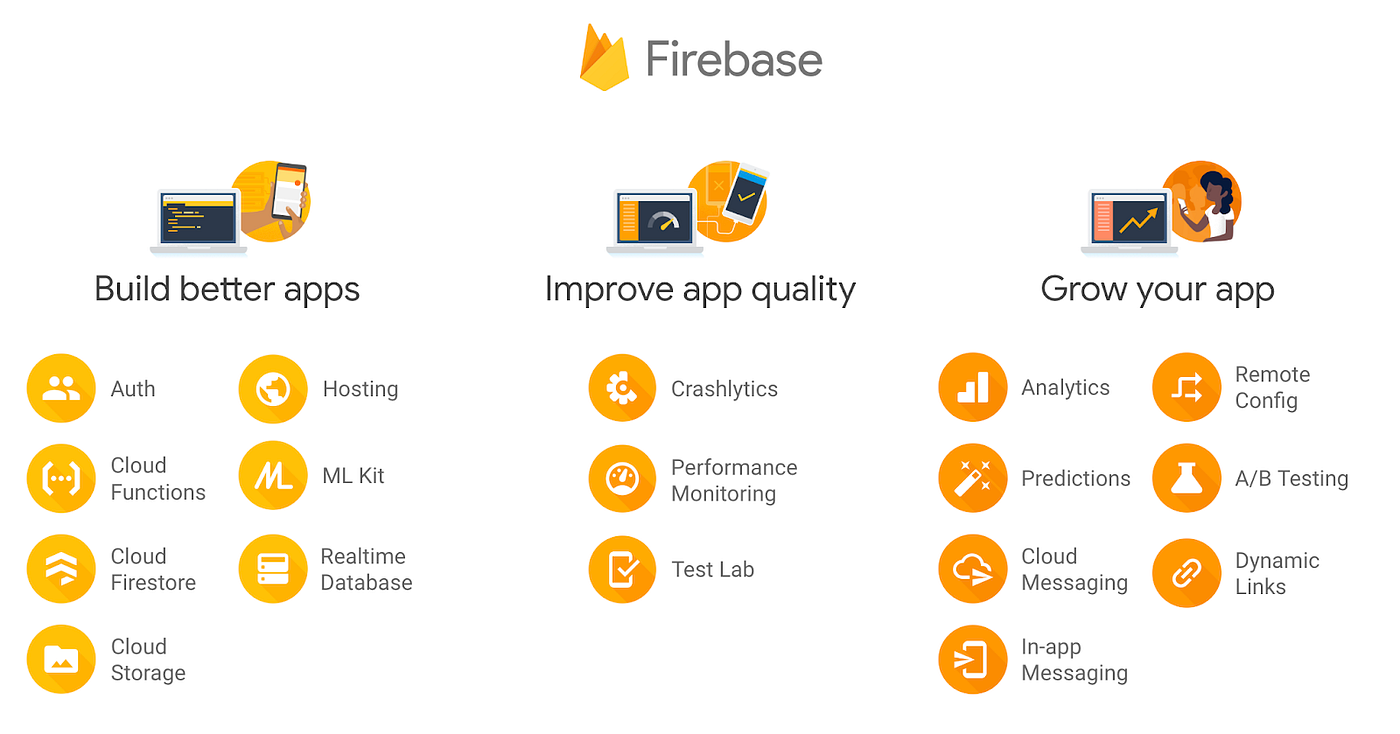
\includegraphics[width=0.9\textwidth]{img/BP-Runt/Data_storing/Firebase/firebase_features.png}
  \caption{Služby platformy Firebase \cite{firebase-meme}}
  \label{fig:firebase-function}
\end{figure}

\noindent \textbf{Firebase Authentication} umožňuje identifikaci uživatelů pomocí různých identifikátorů jako je e-mail a heslo, telefonní číslo, účet Google, Facebook, Twitter, GitHub nebo Apple a vytváření dočasných anonymních účtů. Tato služba umožňuje též pokročilou funkcionalitu jako je změna hesla, ověření přes e-mailovou adresu či telefonní číslo nebo slučování účtů. 

\vspace{0.1cm}
\noindent \textbf{Cloud Firestore} je flexibilní cloudová \gls{NoSQL} databáze, která poskytuje služby pro~ukládání dat, synchronizaci a offline podporu. Data jsou uspořádána do hierarchického datového modelu, ve kterém jsou data uložena v dokumentech. Dokumenty jsou pak zařazeny do kolekcí viz obr. \ref{fig:firestore-data}. Dokumenty podporují mnoho datových typů od čísel po složité vnořené objekty.

\begin{figure}[h]
  \centering
  
\includegraphics[width=0.47\textwidth]{img/BP-Runt/Data_storing/Firebase/structure-data-firestore.png}
  \caption{Model uložení dat v Cloud Firestore \cite{Firestore}}
  \label{fig:firestore-data}
\end{figure}


\vspace{0.1cm}
\noindent \textbf{Firebase Realtime Database} je cloudová \gls{NoSQL} databáze, která poskytuje podobnou funkcionalitu jako Firestore. Hlavní rozdíl oproti Cloud Firestore spočívá ve~struktuře, ve které jsou data uložena v podobě jednoho rozsáhlého \gls{JSON} souboru. 

\vspace{0.1cm}
\noindent \textbf{Firebase Hosting} poskytuje rychlý a bezpečný hosting, který může být použit ke~statickým nebo dynamickým webovým stránkám a \gls{PWA} s použitím bezplatného \gls{SSL} certifikátu. 

\vspace{0.1cm}
\noindent \textbf{Google Analytics for Firebase} slouží k analýze návštěvnosti a chování uživatelů v~aplikaci. Poskytuje podrobné statistiky o skupině uživatelů a její interakce s aplikací.

\vspace{0.1cm}
\noindent \textbf{Firebase Predictions} používá algoritmů umělé inteligence pro analýzu chování uživatelů a~následné předpovídání jejich budoucích akcí.

\vspace{0.1cm}
\noindent \textbf{Firebase Cloud Messaging} je bezplatná služba, která umožňuje odesílání notifikací do mobilních a webových aplikací napříč platformami.

\vspace{0.1cm}
\noindent \textbf{Firebase A/B Testing} je nástroj, který umožňuje provádět experimenty s různými variantami uživatelského rozhraní, zpráv a funkcí, čímž pomáhá k optimalizaci uživatelského zážitku.

\vspace{0.1cm}
\noindent \textbf{Firebase Machine Learning} je nástroj, který umožňuje snadné využití balíčků strojového učení bez potřeby velkých znalostí z oblasti umělé inteligence. V nabídce jsou předtrénované modely pro rozpoznávání textu, překlady, detekce objektů a~další. Zkušeným vývojářům umožňuje použití vlastních TensorFlow Lite modelů. 

%\noindent Toto byl jen zlomek funkcí, teré firebase nabízí.

%síť pro doručování obsahu = CDN - content delivery network 

%Služba \gls{AWS} byla spuštěna v roce 2006 což z ní dělá jednu z prvních svého druhu a dnes se může pyšnit širokou základnou uživatelů.

\subsection{AWS Amplify}

\gls{AWS} je komplexní, široce používanou cloudovou platformu poskytovanou společností Amazon, která nabízí služby výpočetního výkonu, databázového úložiště a~síť pro doručování obsahu. Cloudové služby \gls{AWS} využívají modelu „Pay-as-you-go", kde uživatel platí za využívání služeb dle času a objemu uložených dat. Noví uživatelé mají aktivovaný Free Plan, který je bezplatný na 12 měsíců, pro vyzkoušení služeb, které \gls{AWS} nabízí. \cite{techtarget_AWS} \cite{Amazon_web_service} 

\gls{AWS} Amplify je vývojová platforma, která usnadňuje vývojářům vývoj mobilních a webových aplikací. Tato služba představuje ucelený balík nástrojů a služeb, které pomáhají snadno vytvářet, hostovat a monitorovat běh aplikací. Mezi funkce patří například autorizace, ukládání a synchronizování dat, \gls{UI} komponenty, strojové učení a mnoho dalšího. \gls{AWS} Amplify je vývojový framework založený na JavaScriptu, který se skládá z knihoven, komponentů uživatelského rozhraní a nástrojů \gls{CLI}: \cite{aws-amplify-docs} \cite{javapoint-aws-amplify}   

\begin{itemize}
    \item \textbf{Knihovny:} umožnění připojení, integraci a interakci s cloudovými službami \gls{AWS}. Knihovny umožňují snadno přidat do aplikací bezpečné ověřování, ukládání souborů, ukládání dat, analytiku, notifikace, a další,
    \item \textbf{Komponenty \gls{UI}:} Amplify bylo vytvořeno tak, aby integrovalo \gls{UX} napříč různými platformami, \gls{UI} komponenty jsou pak předpřipravené komponenty uživatelského rozhraní,
    \item \textbf{Nástroje \gls{CLI}:} Tyto nástroje umožňují efektivní správu a aktualizace backendové struktury \gls{AWS}.
\end{itemize}

\section{Shrnutí}

V této kapitole jsme prozkoumali možnosti pro lokální a online ukládání dat. Pro potřeby synchronizace jsem se rozhodl využít cloudové platformy Firebase viz sekce \ref{lab:firebase}, která eliminuje potřebu vytvářet vlastní \gls{API}. Zároveň tato platforma nabízí velký počet funkcí, jako je autorizace uživatele, zasílání notifikací a~ukládání dat, které usnadní a zrychlí vývoj aplikace. Ze dvou typů úložišť (Cloud Firestore, Firebase Realtime Database), které Firebase nabízí, jsem vybral službu Cloud Firestore z~důvodu podpory ukládání komplexnějších dat. Vzhledem k velikosti plánované aplikace by měl stačit bezplatný Spark plan. Při větším počtu uživatelů a míře použití lze přejít na placený Blaze plan.

Pro ukládání uživatelských dat do lokálního úložiště jsem se rozhodl použít knihovnu Hive viz sekce \ref{Hive}, která je mezi vývojáři Flutter aplikací velmi populární. Vzhledem k tomu, že naše data nejsou strukturovaná a Firebase rovněž ukládá data do formátu \gls{NoSQL}, je použití Hive lepší volbou než SQLite. Hive navíc podporuje líné načítání a šifrování, které se též může při vytváření aplikace hodit.


% _____________________________________________________________________________
%
%
%        CHAPTER Návrh
%
% _____________________________________________________________________________
%

\chapter{Návrh aplikace} \label{chapter:navrh}

Obsahem této kapitoly je specifikace funkcionality, návrh datového modelu a uživatelského rozhraní aplikace. Zpočátku kapitoly specifikujeme funkce, které aplikace nabídne svým uživatelům. V další části se zaměříme na organizaci dat, způsoby ukládání a jejich datový model. V závěru kapitoly navrhneme vzhled uživatelského rozhraní a navigaci mezi obrazovkami.

\section{Specifikace funkcionality}

Před samotným vývojem aplikace je nutné specifikovat funkce, které bude vyvíjená aplikace obsahovat. Tato aplikace se bude zaměřovat na tvorbu hierarchicky organizovaných poznámek s možností synchronizace dat mezi více zařízeními. Aplikace bude primárně vytvářena pro platformu Android.

Hierarchická organizace poskytne uživateli libovolný\footnote{Hierarchie bude omezena fyzickými parametry úložiště} počet úrovní, neboť konkrétní počet úrovní může být omezující. Hierarchie by měla být přehledná a umožňovat snadnou organizaci a práci s poznámkami. Poznámky bude též možno přesunout na libovolné místo v hierarchii.

Vzhledem k tomu, že primárně cílíme na mobilní zařízení, je velmi pravděpodobné, že potenciální uživatelé budou chtít používat aplikaci i bez připojení k internetu (například při cestě vlakem). Je tedy důležité zajistit, aby aplikace bezproblémově fungovala bez internetového připojení. Mnoho uživatelů má též více zařízení, ze kterých chtějí své poznámky spravovat. Kromě práce v módu bez připojení k~internetu, je také důležité, umožnit uživatelům synchronizovat svá data mezi více zařízeními. Synchronizace dat bude probíhat prostřednictvím účtu, který si uživatel v aplikaci vytvoří. Je možné, že uživatel bude upravovat data bez připojení k~internetu. V tomto případě mohou vzniknout konflikty, neboli několik různých verzí poznámek, ze kterých nelze jednoznačně určit správnou verzi. Aplikace bude tyto konflikty odhalovat a~následně řešit tak, aby uživatel neztratil data.

I když to není doporučováno, mohou uživatelé uchovávat v poznámkách citlivá data. Je tedy adekvátní tato data bezpečně uchovávat pomocí moderních bezpečnostních standardů. V případě potřeby poznámky uzamknout pinem nebo heslem, kdyby například uživatel někomu půjčil telefon.

Aplikace bude mít veřejně přístupný zdrojový kód a všechny její funkcionality budou dostupné bezplatně. Dalším cílem je vytvořit dobře strukturovat zdrojový kód aplikace tak, aby byla dobře modifikovatelná a nabízela tak dalším vývojářům možnost přidání nové funkcionality.

\section{Případy užití}

V předchozí sekci jsme specifikovali funkce, které by měla vyvíjená aplikace obsahovat. Následující diagram \ref{fig:usecases} reprezentuje všechny funkční požadavky z pohledu uživatele. Aplikace bude plně podporovat režim bez připojení k internetu, uživatelé nemusejí být při používání aplikace registrováni. Aplikaci tedy budou moci používat dva typy uživatelů, a to přihlášení a nepřihlášení uživatelé. Základní funkcionalita zahrnující práci s poznámkami a přizpůsobení aplikace pomocí lokalizace je dostupná oběma typům uživatelů. Přihlášený uživatel má navíc možnost synchronizace poznámek. 

\begin{figure}[h]
  \centering
  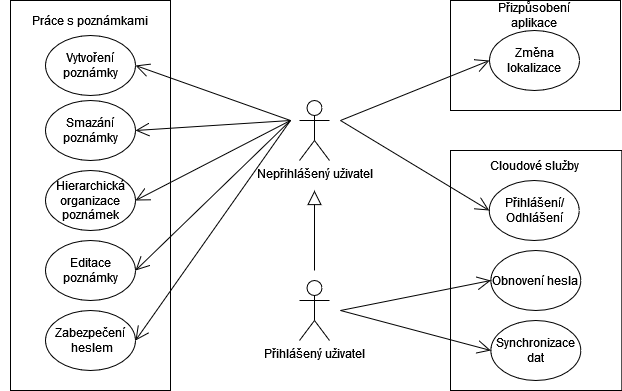
\includegraphics[width=1\textwidth]{img/BP-Runt/Planning/use_case_v01.png}
  \caption{Případy užití aplikace}
  \label{fig:usecases}
\end{figure}

\section{Offline-first návrh}

Jak je zmíněno ve specifikaci aplikace. Je velmi důležité, aby aplikace fungovala i~bez~připojení k internetu. Z tohoto důvodu bude vytvořena offline-first aplikace. V~této aplikaci se uživatel nebude muset přihlásit, aby mohl používat aplikaci. Přihlášení bude povinné až v případě, že by uživatel chtěl synchronizovat nebo zálohovat svá data. Pro získání těchto možností se uživatel bude muset přihlásit.

Offline-first je způsob, který zajišťuje bezproblémové fungování softwaru i bez připojení k internetu. Pro dosažení této funkčnosti je potřeba ukládat data na straně klienta, tedy do lokálního úložiště zařízení. Toto bude dosaženo využitím lokální databáze Hive (viz sekce \ref{Hive}). Při synchronizaci budou data nejdříve uložena do~lokální databáze a až poté zobrazena v uživatelském rozhraní viz obrázek \ref{fig:offline-first-model}.

\begin{figure}[h]
  \centering
  \includegraphics[width=0.8\textwidth]{img/BP-Runt/Planning/offline\_first\_diagram.png}
  \caption{Offline first model ukládání dat}
  \label{fig:offline-first-model}
\end{figure}

\section{Datový model}

Na následujícím obrázku \ref{fig:data-model} je znázorněný datový model, který by mohl být využit ve vytvářené aplikací. V návrhu jsou znázorněny entity, jejich atributy a relace mezi nimi. První entitou je uživatel, který bude obsahovat identifikátor, dle kterého bude uživatel ověřovat svou identitu. Dalšími atributy uživatele bude údaj o vlastněných souborech, poslední synchronizaci, preferovaném tématu a jazyce. Každý uživatel pak může vlastnit libovolný počet souborů, což je druhá entita diagramu. Soubor může být dvou druhů, a to typu adresář nebo poznámka. Soubory mají atributy unikátního identifikátoru, jména a čas poslední změny. Poznámka má navíc oproti souboru ještě atributy obsahu poznámky, jestli je poznámka zamčena a případné heslo. Adresář obsahuje seznam odkazů na soubory, které jsou jeho potomky.

\begin{figure}[h]
  \centering
  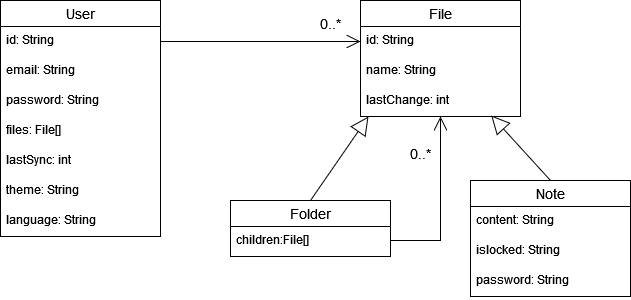
\includegraphics[width=0.9\textwidth]{img/BP-Runt/Planning/data-model-updated.png}
  \caption{Plánovaný datový model aplikace}
  \label{fig:data-model}
\end{figure}

V kapitole \ref{chap:data} jsme určili, jaké technologie budou využity pro ukládání dat. Konkrétně jsme zvolili databázi Hive pro lokální ukládání dat a cloudové úložiště Firestore. Ačkoliv obě databáze patří do kategorie \gls{NoSQL} databází, jejich styl ukládání dat se liší. Při implementaci tedy bude nezbytné adaptovat tento datový model na~specifika dané technologie tak, aby byla zajištěna konzistence dat v obou úložištích.

\section{Uživatelské rozhraní}

Před zahájením vývoje je též vhodné navrhnout vzhled a uspořádání komponent na obrazovkách. Zároveň je důležité zvážit, jak bude uživatel interagovat s aplikací a jaká bude navigace mezi obrazovkami. Cílem návrhu uživatelského rozhraní je~vytvořit prostředí, které bude uživatelsky přívětivé a ovládání bude pro uživatele intuitivní. 

Pro návrh uživatelských rozhraní jsem využil aplikace Figma\footnote{https://www.figma.com/}, ve které jsem vytvořil návrhy rozložení jednotlivých obrazovek. Jednotlivé návrhy jsou zobrazeny na obrázcích \ref{fig:planning_UI_1}, \ref{fig:planning_UI_2} a \ref{fig:planning_UI_3}. Při návrhu jsem využil knihovny Material 3 Design kit, jejíž komponenty budou použity při tvorbě aplikace. Pro návrh uspořádání jednotlivých obrazovek jsem vytvořil drátový model mobilní aplikace viz obrázek \ref{fig:wireframing-diagram}, ve kterém je zobrazeno, jak bude možné se pohybovat mezi obrazovkami.

\begin{figure}[h!]
  \centering
  \begin{minipage}[h]{0.30\textwidth}
    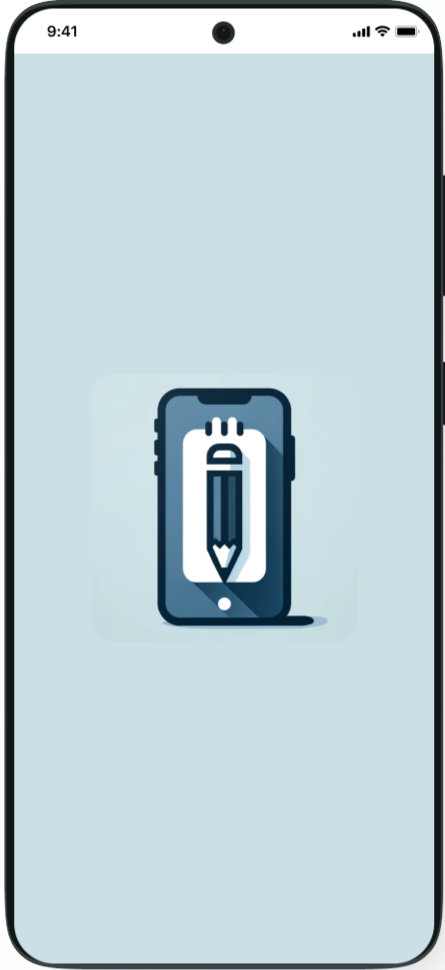
\includegraphics[width=\textwidth]{img/BP-Runt/Planning/UI/Splash screen_upravene.png}
  \end{minipage}
  \hfill
  \begin{minipage}[h]{0.30\textwidth}
    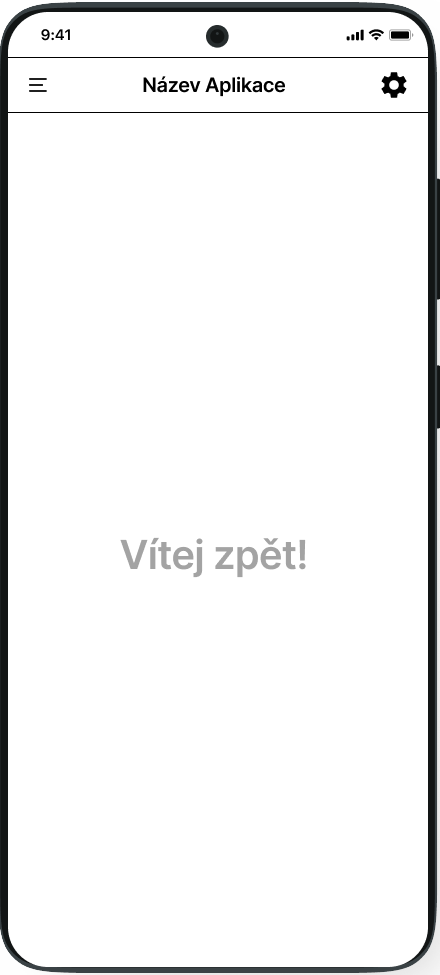
\includegraphics[width=\textwidth]{img/BP-Runt/Planning/UI/Home Screen_edited.png}
  \end{minipage}
  \hfill
  \begin{minipage}[h]{0.30\textwidth}
    \includegraphics[width=\textwidth]{img/BP-Runt/Planning/UI/Nastavení_edited.png}
  \end{minipage}
  \caption{Návrh uživatelského rozhraní: inicializační obrazovka, úvodní obrazovka a nastavení}
  \label{fig:planning_UI_1}
\end{figure}

Při spuštění aplikace se uživateli zobrazí inicializační obrazovka s logem (obrázek \ref{fig:planning_UI_1} vlevo). Potom, co se aplikace inicializuje, se uživateli zobrazí úvodní obrazovka (obrázek \ref{fig:planning_UI_1} uprostřed). Na této obrazovce bude mít uživatel možnost otevřít nastavení (obrázek \ref{fig:planning_UI_1} vpravo) a ovládací menu (obrázek \ref{fig:planning_UI_2} vlevo), ve~kterém bude zobrazena hierarchická struktura poznámek s možností přihlášení uživatele. Hierarchická struktura může být realizováno knihovnou \texttt{flutter\_fancy\_tree\_view} na obrázku \ref{fig:treeView}.

\begin{figure}[h]
  \centering
  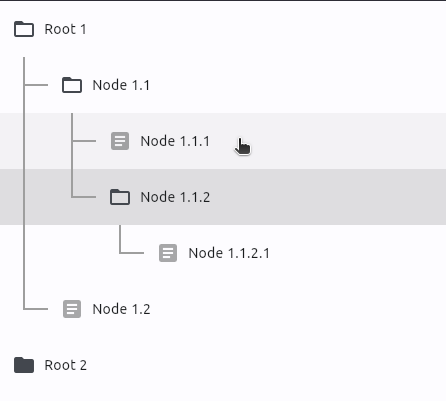
\includegraphics[width=0.5\textwidth]{img/BP-Runt/Planning/UI/treeView.png}
  \caption{Stromové zobrazení hierarchické struktury \cite{flutter-tree-view}}
  \label{fig:treeView}
\end{figure}

Hierarchii poznámek bude mít uživatel možnost organizovat již ve stromové struktuře. Soubory budou moci být přesunuty, přejmenovány, smazány a v adresářích bude možné vytvářet nové adresáře a poznámky. Tento strom bude též sloužit pro navigaci. Při kliknutí na adresář bude uživatel přesměrován na příslušnou stránku s načteným obsahem souboru (viz obrázek \ref{fig:planning_UI_2}). Při otevření adresáře bude zobrazen seznam potomků adresáře s možností úprav a vytváření nových souborů. V případě poznámku bude uživatel přesměrován to editoru formátovaného textu, kde bude načten obsah poznámky.  

\begin{figure}[h!]
  \centering
  \begin{minipage}[h]{0.30\textwidth}
    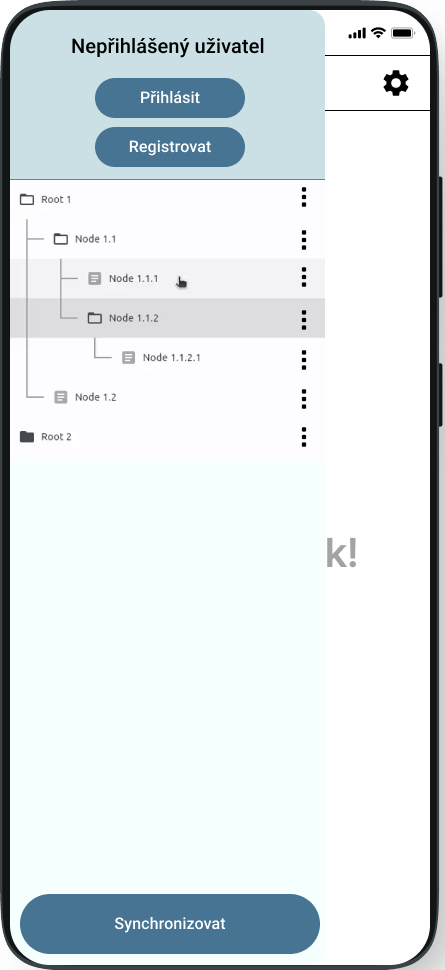
\includegraphics[width=\textwidth]{img/BP-Runt/Planning/UI/Opened_drawer_upravene.png}
  \end{minipage}
  \hfill
  \begin{minipage}[h]{0.30\textwidth}
    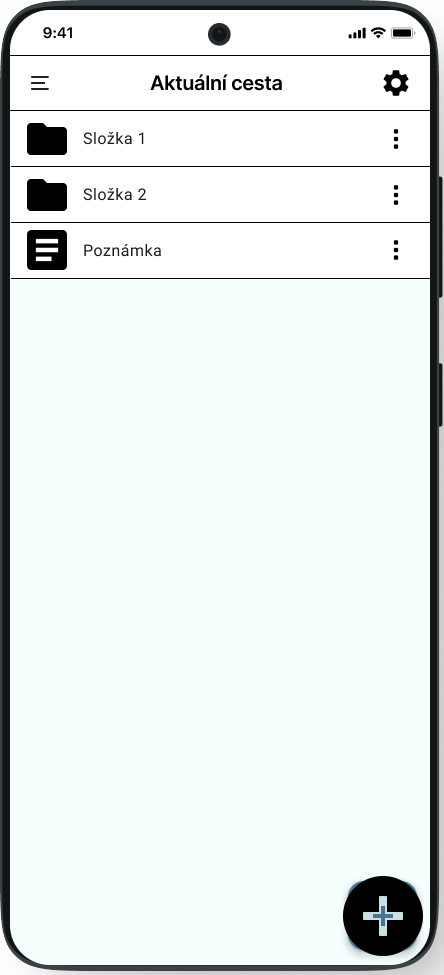
\includegraphics[width=\textwidth]{img/BP-Runt/Planning/UI/ListView_edited.png}
  \end{minipage}
  \hfill
  \begin{minipage}[h]{0.30\textwidth}
    \includegraphics[width=\textwidth]{img/BP-Runt/Planning/UI/Poznámka_upravene.png}
  \end{minipage}
  \caption{Návrh uživatelského rozhraní: otevřené vysouvací menu, obsah složky a editace poznámky}
  \label{fig:planning_UI_2}
\end{figure}

\newpage
Pro~přihlášení se budou ve vysouvacím menu nacházet tlačítka Přihlášení a~Registrace. Tato tlačítka budou přesouvat uživatele na příslušné obrazovky pro přihlášení a~registraci, mezi kterými bude možno se přesouvat (viz obrázek \ref{fig:planning_UI_3}). Na~obrazovce přihlášení bude odkaz na stránku, která bude odesílat e-mail pro obnovu hesla, pokud by uživatel své heslo zapomněl.   


\begin{figure}[h!]
  \centering
  \begin{minipage}[h]{0.30\textwidth}
    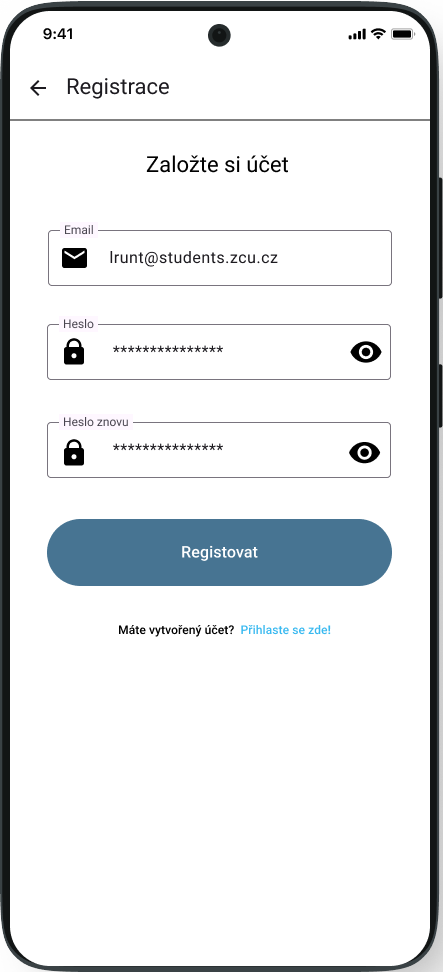
\includegraphics[width=\textwidth]{img/BP-Runt/Planning/UI/Registrace_edited.png}
  \end{minipage}
  \hfill
  \begin{minipage}[h]{0.30\textwidth}
    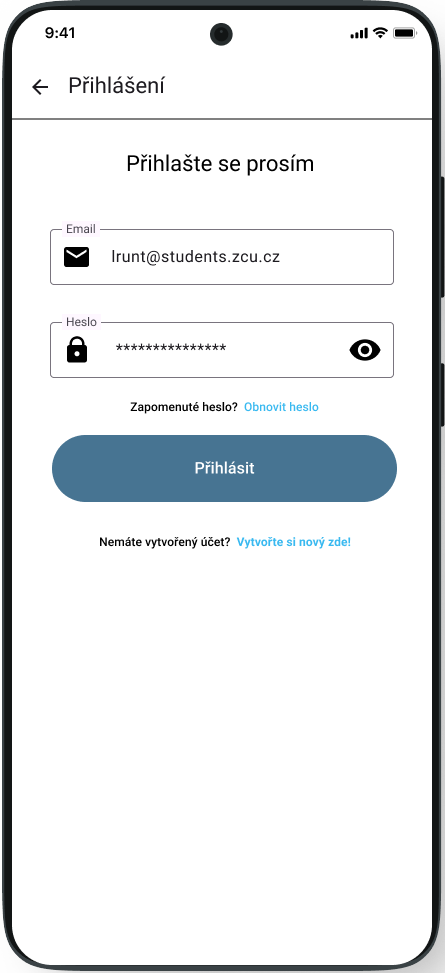
\includegraphics[width=\textwidth]{img/BP-Runt/Planning/UI/Přihlášení_edited.png}
  \end{minipage}
  \hfill
  \begin{minipage}[h]{0.30\textwidth}
    \includegraphics[width=\textwidth]{img/BP-Runt/Planning/UI/Obnovení hesla_upravene.png}
  \end{minipage}
  \caption{Návrh uživatelského rozhraní: registrace nového uživatele, přihlášení a obnova hesla}
  \label{fig:planning_UI_3}
\end{figure}


\begin{landscape}

\begin{figure}[h]
  \centering
  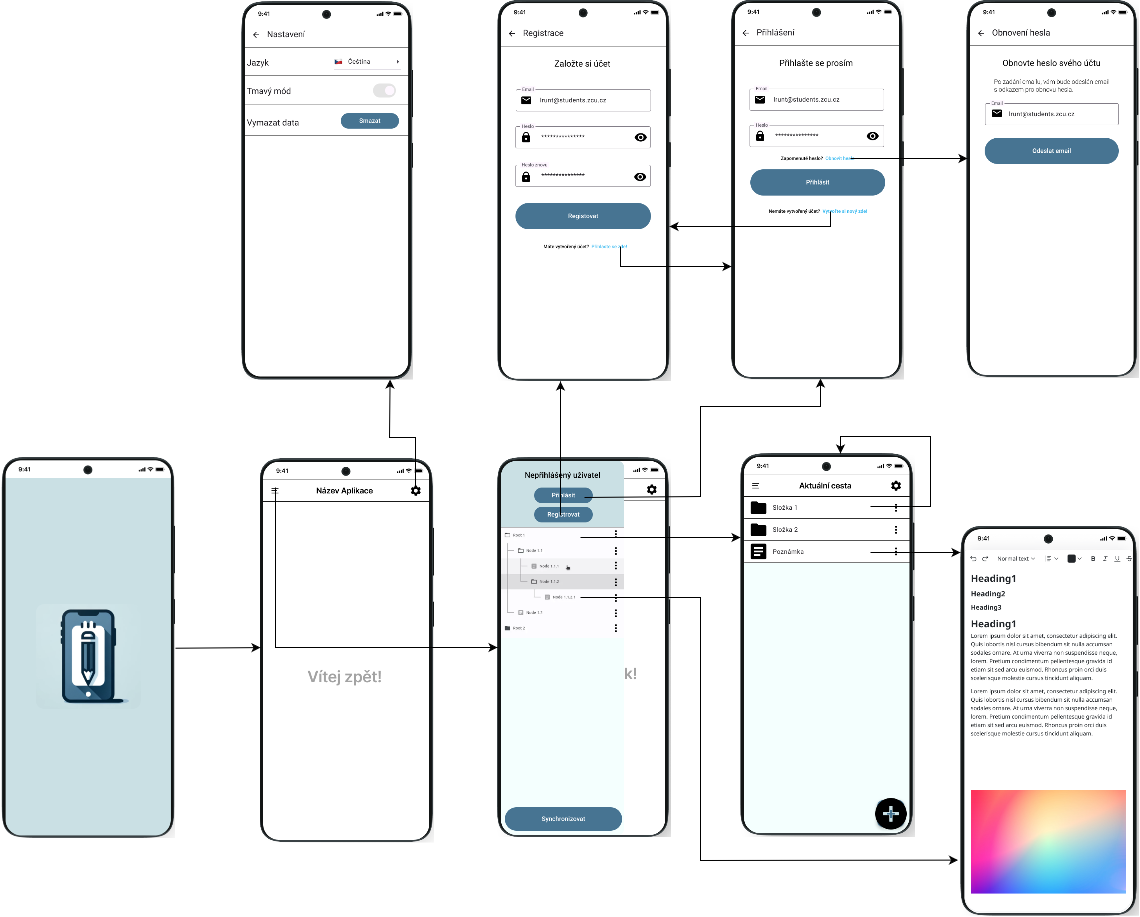
\includegraphics[width=1.2\textwidth]{img/BP-Runt/Planning/UI/drátový_model.png}
  \caption{Drátový model mobilní aplikace}
  \label{fig:wireframing-diagram}
\end{figure}

\end{landscape}


% _____________________________________________________________________________
%
%
%        CHAPTER Implementation
%
% _____________________________________________________________________________
%
\chapter{Implementace}

Následující kapitola se zabývá implementací vyvíjené aplikace. Na začátku kapitoly si popíšeme strukturu projektu. Následně se přesuneme k organizaci a ukládání lokálních dat. Od lokálního ukládání dat se přesuneme k využití cloudových služeb Firebase a synchronizaci dat. V závěru kapitoly se budeme věnovat vzhledu aplikace a platformám, na kterých je aplikace zveřejněna.

\section{Struktura projektu}

 Projekt má charakteristickou Flutter strukturu. V následující části si popíšeme důležité části této struktury:

\begin{itemize}
    \item \texttt{assets/} je adresář, ve kterém jsou obsaženy všechny multimediální soubory, které aplikace využívá,
    \item \texttt{android/} je adresář obsahující vše potřebné pro sestavení Androidové aplikace včetně Gradle skriptů a Android manifestu,
    \item \texttt{web/} je adresářem, kde Flutter ukládá všechny soubory potřebné pro běh webové aplikace, 
    \item \texttt{lib/} je hlavní adresář, ve kterém je vývojářem napsaný zdrojový kód aplikace, 
    \item \texttt{test/} je složka, která obsahuje všechny automatické testy. Více o testech v~kapitole \ref{chap:testing},
    \item \texttt{firebase.json} je soubor popisující konfiguraci hostování webové aplikace,
    \item \texttt{package.json} je soubor, který Node.js používá k zaznamenání verze všech balíčků,
    \item \texttt{pubspec.yaml} je soubor, ve kterém jsou definovány všechny knihovny a~závislosti.
    
\end{itemize}

\subsection{Adresář lib}

Adresář \texttt{lib} hraje ve Flutter projektech důležitou roli, jelikož obsahuje většinu zdrojového kódu, který vývojář napíše. Tento kód je společný pro všechny platformy. Během procesu sestavování aplikace pro konkrétní platformu se tento multiplatformní kód kompiluje do nativního kódu jednotlivých platforem.

Při tvorbě rozsáhlých projektů je vhodné rozhodnout, jak budeme náš projekt strukturovat. Struktura adresáře \texttt{lib} má zásadní vliv na přehlednost a udržitelnost projektu. Existuje více způsobů, jak projekt přehledně strukturovat. V našem případě byla zvolena struktura, ve které jsou zdrojové soubory uspořádány dle jejich typu na komponenty, obrazovky, servisy, lokalizační soubory, model a data:

\begin{itemize}
    \item \texttt{components/} je adresář obsahující všechny předdefinované komponenty použité v obrazovkách aplikace,
    \item \texttt{data/} v tomto adresáři se nachází část zdrojového kódu, který manipuluje s lokální databází. Tyto třídy čtou, zpracovávají a ukládají data do lokálního úložiště zařízení,
    \item \texttt{l10n/} (zkratka pro lokalizaci) obsahuje soubory potřebné pro lokalizaci aplikace. Každý jazyk má v tomto adresáři vlastní soubor s příslušnými překlady,
    \item \texttt{screens/} zde se nachází zdrojový kód definující jednotlivé obrazovky aplikace,  
    \item \texttt{services/} tento adresář obsahuje logiku aplikace zahrnující autentifikaci, editaci hierarchické struktury, synchronizace a mnohé další,
    \item \texttt{boxes.dart} je soubor obsahující všechny Hive boxy pro lokální ukládání lokálních dat,
    \item \texttt{firebase$\_$options.dart} obsahuje konfiguraci připojení ke službě Firebase pro různé platformy,
    \item \texttt{constants.dart/} je složka, ve které jsou uloženy všechny konstanty použité v aplikaci, 
    \item \texttt{main.dart} je soubor, ve kterém se Flutter aplikace inicializuje a spouští.
\end{itemize}

\section{Ukládání a editace lokálních dat}

V této části kapitoly se zaměříme na základní funkcionalitu aplikace bez připojení k internetu. Nejdříve si vysvětlíme, jak jsou ukládaná lokální data. V dalších sekcích probereme implementaci hierarchické struktury a editoru poznámek.

\subsection{Lokální ukládání}

Pro lokální ukládání byla použita již zmíněná databáze Hive, která pracuje s boxy. Box je schopen uložit primitivní datové typy nebo objekty, pokud je k boxu připojený vygenerovaný TypeAdapter příslušného objektu. Ukládání objektů jsem využil v~případě ukládání hierarchické struktury. V následujícím schématu \ref{fig:local-data-model} je zobrazeno, jaká data jsou uložena v konkrétních boxech.

\begin{figure}[h]
  \centering
  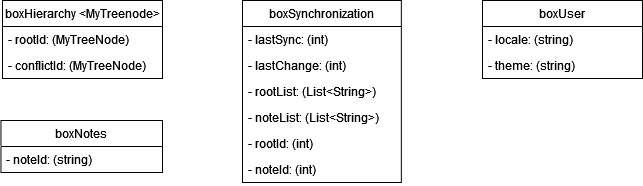
\includegraphics[width=1\textwidth]{img/BP-Runt/Planning/local-data-model.png}
  \caption{Model pro ukládání lokálních dat}
  \label{fig:local-data-model}
\end{figure}

Lokální data jsem uložil do čtyř boxů, podle toho, s jakým účelem se data používají. Každý box ovládá jedna třída v adresáři \texttt{data/}. Hierarchickou strukturu ukládá \texttt{boxHierarchy} a \texttt{boxNotes} ukládá obsah poznámek. Data v těchto boxech se ukládají pomocí identifikátoru (cesty) objektů. Data, která jsou potřeba pro~správnou synchronizaci dat, jsou uložena v \texttt{boxSynchronization}. Pro uložení uživatelských preferencí slouží \texttt{boxUser}.

\subsection{Hierarchická struktura}

Hierarchická struktura hraje v naší aplikaci klíčovou roli. V rámci implementace jsem se rozhodl tuto strukturu znázornit dvěma způsoby. Prvním způsobem je pomocí treeView ve vysouvacím menu. Pro treeView neexistuje žádná defaultní knihovna Flutteru, a tak jsem využil knihovny \texttt{flutter\_fancy\_tree\_view}\footnote{https://pub.dev/packages/flutter\_fancy\_tree\_view}, která nabízí vykreslení hierarchického stromu. K použití této knihovny je potřeba přizpůsobit datový model, přesněji adresáře a poznámky, potřebám této knihovny. Tato knihovna pracuje s instancemi, které obsahují atributy \texttt{title} a \texttt{children} viz zdrojový kód \ref{code:myTreeNode}. Při inicializaci widgetu se pak vytváří instance \texttt{TreeControlleru} do~které se inicializuje \texttt{List} kořenů stromu viz zdrojový kód \ref{code:treeController}. 

\newpage

\begin{code}{java}{MyTreeNode - uzel hierarchické struktury \label{code:myTreeNode}}
class MyTreeNode {
    final String title;
    final List<MyTreeNode> children;

    const MyTreeNode({
        required this.title,
        this.children = const <MyTreeNode>[],
    });
}
\end{code}

Druhým způsobem hierarchického zobrazení je seznam potomků, který je implementován pomocí \texttt{ListView}. Pokud uživatel v hierarchické struktuře klikne na~adresář, jsou na hlavní stránce zobrazeny potomci adresáře, který uživatel stiskl. Na~této stránce má uživatel možnost procházet adresáře i poznámky.

\begin{code}{java}{Vytvoření instance TreeControlleru \label{code:treeController}}
final List<MyTreeNode> roots = hierarchyDb.getRoots();
final treeController = TreeController<MyTreeNode>(
  roots: roots,
  childrenProvider: (MyTreeNode node) => node.children,
);
\end{code}

V hierarchické struktuře jsou definovány dva typy uzlů, jejíž typ určuje atribut \texttt{isNote}. Každý uzel je instancí \texttt{MyTreeNode}, které jsem přidal několik atributů, aby šla hierarchická struktura snadno editovat a byla poskytnuta příslušná funkce. Instance \texttt{MyTreeNode} obsahuje následující atributy:

\begin{itemize}
    \itemsep0em 
    \item \textbf{id:} Jedinečný identifikátor uzlu, který byl navržen pro efektivní prohledávání a organizaci hierarchické struktury. Identifikátor instance obsahuje cestu ve~formátu \texttt{|<id\_kořenu>|<id\_uzlu>|<id\_listu>}, kde každé ID odděluje vertikální čára,
    \item \textbf{title:} Název poznámky nebo adresáře, který je zobrazen v uživatelském rozhraní. Nesmí obsahovat znak '|' (oddělovač v cestě) a '/' (znak se speciální funkcí ve Firestore),
    \item \textbf{isNote:} Značí, zda je uzel adresářem či poznámkou. Na základě této vlastnosti se určují funkce, dostupné pro daný uzel,
    \item \textbf{children:} Seznam potomků uzlu. Do seznamu se ukládají celé instance uzlů,
    \item \textbf{isLocked:} Určuje, zda je uzel chráněn heslem, 
    \item \textbf{password:} Hash hesla zamčeného uzlu, vytvořený algoritmem \gls{SHA}-256. V~odemčených uzlech nastavena hodnota \texttt{null}. 
\end{itemize}


Metody pro organizaci hierarchické struktury jsou implementovány v souboru \texttt{services/node\_service.dart}. V rámci naší aplikace je implementována metoda pro odstranění, přejmenování, vytvoření nové složky a poznámky (jen u adresářů), přesunutí a uzamknutí/odemknutí (jen u poznámek). Při operacích se kontroluje jméno souboru tak, aby jméno souboru nebylo prázdné, neobjevovaly se~nepovolené znaky '|' a '/' a aby díky operaci nevznikly dva uzly se stejným jménem ve~stejném adresáři a tím pádem i se stejným identifikátorem. Při odstraňování souborů je nutno zkontrolovat jeho typ. V případě poznámky musíme odstranit i~obsah samotné poznámky. Při existenci potomků musíme tento postup opakovat u každého následujícího potomka. U přejmenování a přesouvání musíme zajistit správnou změnu cest v identifikátorech uzlů.

\subsection{Editace poznámek}

Většina aplikací pro tvorbu poznámek nabízí rozsáhlé možnosti formátování a obsahu poznámek. Pro poskytnutí srovnatelné úrovně uživatelské přívětivosti formátování textu, jsem se rozhodl využít knihovnu \texttt{flutter\_quill}\footnote{https://pub.dev/packages/flutter\_quill}, pro kterou jsou pravidelně vydávány nové verze. Tento editor formátovaného textu pracuje s~daty ve formátu \gls{JSON}. Aby uživatel neztratil žádná data, která v aplikaci vytvoří, ukládám obsah poznámky při každé změně do lokálního úložiště zařízení. Nová data přepisují starou verzi poznámky společně s aktualizací časové značky poslední úpravy. 

\section{Integrace služeb Firebase}

Vytvářená aplikace využívá cloudových služeb Firebase. V této sekci si představíme služby, které vytvářená aplikace využívá. V rámci této sekce si také vysvětlíme, jak funguje synchronizace dat, která s těmito službami úzce souvisí.

\subsection{Autentizace}

Aby uživatelé mohli synchronizovat svá data, je nutné uživatele nějakým způsobem identifikovat. V naší aplikaci je k tomuto účelů využita cloudová služba Firebase Authentication (viz sekce~\ref{lab:firebase}), která dokáže umožnit přístup k datům pouze autorizovaným uživatelům.

Autentizační proces naší aplikace podporuje přihlášení kombinací e-mailu a~hesla a přihlášení účtem Google. Pro případ, že uživatel zapomene své heslo, jsem využil služby Firebase odeslat e-mail s odkazem na stránku, kde uživatel může své heslo změnit. Obsah tohoto e-mailu lze libovolně změnit, dle potřeb vytvářené aplikace. 

Implementace Firebase Auth v našem projektu vyžadovala přidání závislosti \texttt{firebase\_auth} a konfigurování propojení s vytvořeným Firebase projektem (návod na konfiguraci viz příloha \ref{app:firebase-configuration}). Po konfiguraci a přidání závislosti lze využívat instanci \texttt{Firebase.auth}, která zprostředkovává přístup ke všem funkcím a udržuje stav uživatelova přihlášení. Tato instance je inicializována již na začátku běhu aplikace a postupně předávána v parametrech jednotlivých tříd, pro lepší usnadnění testování a lepší udržitelnost kódu. 

V logické vrstvě aplikace ve třídě \texttt{auth\_service.dart} jsou implementovány metody pro registraci, přihlášení, odhlášení a odeslání e-mailu pro změnu hesla. Pokud nastane při přihlašování chyba (například uživatel nebude mít přístup k internetu) vrátí metody chybový kód, který je následně namapován na chybové hlášení srozumitelné pro uživatele. K zobrazení chybových hlášení jsem použil komponentu \texttt{SnackBar}.  

\subsection{Cloud Firestore}

Pro ukládání uživatelských dat do cloudové databáze bylo nutné přizpůsobit datový model požadavkům databáze Firestore, která pracuje s kolekcemi a dokumenty. Vytvořený model využívá údaje z Firebase Auth tak, že každý uživatel vlastní kolekce s vlastním identifikačním číslem. Tím má uživatel zajištěn přístup ke svým datům. Datový model databáze Firestore je zobrazen na následujícím obrázku \ref{fig:firestore-data-model}. Komunikaci s databází zajišťuje třída \texttt{firestore\_service.dart}, která mimo jiné obsahuje logiku synchronizace a s tím spojené detekování konfliktů.

\begin{figure}[h]
  \centering
  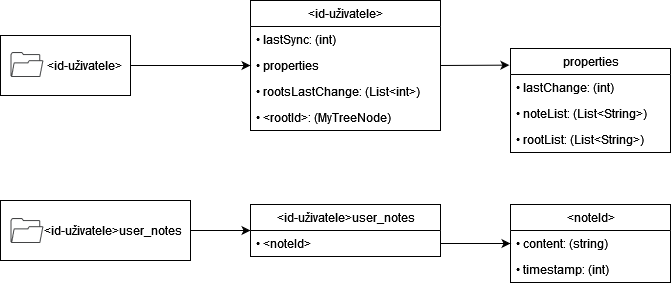
\includegraphics[width=1\textwidth]{img/BP-Runt/Planning/Firebase-data-model.png}
  \caption{Datový model databáze Firestore}
  \label{fig:firestore-data-model}
\end{figure}

\newpage

\subsection{Synchronizace dat}

Před implementací synchronizace bylo rozmýšleno mezi synchronizací s užitím časových značek a historií změn. Z těchto dvou metod byla zvolena metoda časových značek. Tento způsob uchovává časový údaj o poslední synchronizaci a poslední změně každého souboru. Dle časových údajů se pak rozhoduje, zda budou data stažena do lokálního zařízení nebo nahrána na cloudové úložiště. Pomocí časových značek lze také odhalit potenciální konflikty. Pokud je poslední změna souboru provedena před poslední synchronizací, byl soubor nezměněn a může se přepsat novými daty. Pokud je však poslední změna souboru datována až po synchronizaci u lokálního i na cloudu uloženém souboru, je velmi pravděpodobné, že se jedná o~konflikt. 

\subsection{Řešení konfliktů}

Pokud je při synchronizaci odhalen potencionální konflikt, je lokální verze těchto dat uložena s časovou značkou ve formátu \texttt{<jméno souboru><časová značka>} do části lokální databáze pro správu konfliktů. Následně jsou data, která se zobrazují uživateli v hierarchickém stromě přepsána verzí dat z databáze Firestore. Po~synchronizaci má tak uživatel přístup k oběma verzím poznámek. Data, kterých se~konflikt týká, lze zobrazit v nastavení, stisknutím tlačítka Konflikty.    

\section{Přizpůsobení a vzhled}

Při vývoji jsem se snažil zapracovat též na příjemném a konzistentním vzhledu, který se bude uživatelům líbit a bude charakterizovat vytvářenou aplikaci. Snahou také bylo umožnit uživatelům volbu preferovaného jazyka a výběr mezi světlým a~tmavým režimem. V další části si rozebereme, jakým způsobem byl navržen vzhled a přepínání jednotlivých preferencí.

\subsection{Logo a úvodní obrazovka}

Každá aplikace by měla mít své logo a název, který ji bude charakterizovat a odlišovat od~ostatních aplikací. Aplikaci jsem pojmenoval názvem \textit{Notes}, což je slovo, které má svůj význam v češtině i angličtině. Vzhledem k tomu, že nemám dostatečné umělecké cítění, využil jsem pro vytvoření loga, zobrazeného na obrázku \ref{fig:logo}, umělé inteligence DALL-E. Při založení Flutter projektu se aplikaci nastaví výchozí Flutter logo. Pro změnu loga aplikace byla použita knihovna \texttt{flutter\_launcher\_icons}\footnote{https://pub.dev/packages/flutter\_launcher\_icons}, pro kterou jsem v souboru \texttt{pubspec.yaml} definoval verzi a obrázek, ze kterého se~ikony vytvoří. Následně jsem použil příkaz pro vygenerování ikony pro všechny distribuce.

Při spouštění se aplikace inicializuje. Při inicializování je implicitně nastavena čistě bílá obrazovka. Uživatel pak má pocit, že aplikace nefunguje správně. Tuto stránku jsem tedy nechtěl ponechat bílou, a proto jsem na tuto stránku přidal logo aplikace s použitím knihovny \texttt{flutter\_native\_splash}\footnote{https://pub.dev/packages/flutter\_native\_splash}. Pro nadefinování úvodní obrazovky je opět potřeba upravit \texttt{pubspec.yaml}, ve kterém můžeme nastavit obrázek a pozadí, které se uživateli při inicializaci zobrazí. S~použitím příkazu lze pak vygenerovat úvodní obrazovku pro všechny distribuce.

\begin{figure}[h!]
  \centering
  
\includegraphics[width=0.5\textwidth]{img/BP-Runt/Implementation/note_taking_app_logo.png}
  \caption{Logo aplikace}
  \label{fig:logo}
\end{figure}

\subsection{Lokalizace}

Vytvořená aplikace obsahuje podporu a překlady anglického a českého jazyka. Pro lokalizaci je využita knihovna \texttt{intl 0.18.1}\footnote{https://pub.dev/packages/intl}, která je přidána v seznamu závislostí s~povolením automatického generování zdrojového kódu. Lokalizační soubory s překlady jsou uloženy v adresáři \texttt{lib/l10n/}. Pro každý jazyk je vytvořen samostatný lokalizační soubor ve formátu \gls{ARB}, který obsahuje mapu klíčů a překladů. V případě vyvíjené aplikace se jedná o soubory \texttt{app$\_$en.arb} pro angličtinu a \texttt{app$\_$cs.arb} pro češtinu. 

Pro používání internacionalizace je dále potřeba vytvořit konfigurační soubor \texttt{l10n.yaml} viz zdrojový kód \ref{code:l10n-setup}, ve kterém první řádka specifikuje cestu, kde se nacházejí lokalizační soubory. Na druhé řádce je určen šablonový soubor. Tento soubor obsahuje všechny definice textových řetězců s popisy, kde se daný textový řetězec používá. Jako šablonový soubor se nejčastěji používá anglický lokalizační soubor. Poslední řádkou v konfiguraci definujeme název souboru, kam se nám budou generovat jednotlivé překlady. Překlady lze generovat příkazem: \texttt{flutter gen-l10n}.

\begin{code}{java}{Konfigurační soubor l10n.yaml \label{code:l10n-setup}}
// Cesty k lokalizačním souborům.
arb-dir: lib/l10n
// Určení šablonového souboru.
template-arb-file: app_en.arb
// Jméno souboru, kam se budou generovat překlady.
output-localization-file: app_localizations.dart
\end{code}

K přepínaní jazykových preferencí byla vytvořena třída \texttt{language.dart}, která je uložena v adresáři \texttt{model}. Instance třídy obsahuje atribut emotikonu vlaky (\texttt{flag}), název jazyka (\texttt{name}) a kód jazyka dle normy ISO 639-1 (\texttt{langCode}). Výchozím jazykem aplikace je angličtina. Při změně jazyka je kód preferovaného jazyku uložen do lokální databáze.

\subsection{Barevné palety a přepínání témat}

Všichni uživatelé nemusejí preferovat světlá témata. Zejména pak ve večerních hodinách může být příjemnější sledovat displej méně osvětlený než přesvícený. Z těchto důvodů jsem se rozhodl do aplikace přidat výběr mezi světlým a tmavým módem. 

Při definování palety jednotlivých zobrazení jsem se snažil využít barev, které byly užity při vytváření loga aplikace, aby bylo docíleno konzistence. Při vytváření barevných palet pro oba módy jsem využil stránky Material Theme Builder\footnote{https://m3.material.io/theme-builder\#/custom}, která zobrazuje, jak barvy ovlivní vzhled jednotlivých komponent. Vývojář pak může z~definovaných barev vygenerovat barevné palety pro obě témata. Tyto palety jsem vygeneroval a následně uložil jako konstanty do souboru \texttt{constants.dart}. 

Pro umožnění změny tématu jsem vytvořil třídu \texttt{theme.dart}, která využívá funkce poskytovatele stavu (Provideru) pro centralizovanou správu režimu. Tato třída uchovává informace o aktuálním tématu, světlém tématu a~tmavém tématu a~obsahuje metody \texttt{setThemeMode}, \texttt{setLightScheme} a \texttt{setDarkScheme}, kterými lze režim měnit. Instance \texttt{ThemeProvider} je vytvořena při inicializaci aplikace s použítím \texttt{ChangeNotifierProvider} a \texttt{Customer} (viz zdrojový kód \ref{code:theme-listener}), což poskytuje správné téma napříč widgetovým stromem. Pokud pak nastane změna, všichni posluchači jsou informováni o změnách, které nastaly. 

V souboru \texttt{main.dart} je pak mód inicializován na systémový mód uživatele. Při změně preferencí se uživatelské preference ukládají do lokální databáze aplikace a při opětovném spuštění programu se inicializuje hodnota z lokální databáze.

\newpage

\begin{code}{java}{Inicializace ChangeNotifierProvider instance ThemeProvider \label{code:theme-listener}}
 @override
  Widget build(BuildContext context) {
    return ChangeNotifierProvider(
      create: (context) => ThemeProvider(themeMode: initialThemeMode, userDb: db),
      child: Consumer<ThemeProvider>(
        builder: (context, themeProvider, child) {
          return MaterialApp(
            title: 'Notes',
            theme: ThemeData(useMaterial3: true, colorScheme: themeProvider.lightScheme),
            darkTheme: ThemeData(useMaterial3: true, colorScheme: themeProvider.darkScheme),
            themeMode: themeProvider.themeMode,
            home: MainScreen(
            ),
          );
        },
      ),
    );
  }
\end{code}

\section{Distribuce}

S použitím technologie Flutter se mi podařilo vytvořit verzi aplikace pro platformu Android a progresivní webovou aplikaci. Obě verze sdílí většinu zdrojového kódu. Většina změn se~týká vizuálního aspektu aplikace, konfigurace propojení se službou Firebase a změny závislostí knihoven.

\subsection{Android}
Pro mobilní verzi s Androidem byl vygenerován \gls{APK} soubor pomocí příkazu \texttt{flutter build apk}. Aplikace vyžaduje alespoň Android 6.0 Marshmallow (\gls{API} level 23). Návod na instalaci je uveden v příloze \ref{app:install-manual} bakalářské práce. 

\subsection{Webová aplikace}
Pro distribuci webové aplikace bylo potřeba upravit inicializaci spojení se~službou Firebase a změnit závislostí v rámci přihlášení pomocí účtu Google. Následně byl vygenerován nativní kód webové aplikace příkazem \texttt{flutter build web}. Vygenerované zdrojové soubory byly umístěny na hostovaný Firebase server. Postup konfigurace a nastavení hostování je popsán v~příloze~\ref{app:firebase-configuration}. 


% _____________________________________________________________________________
%
%
%        CHAPTER Testing
%
% _____________________________________________________________________________
%
\chapter{Testování Aplikace} \label{chap:testing}

Nezbytnou součástí vývoje je testování. Testy nám sice neříkají nic o tom, že je~software bezchybný, avšak mohou nám pomoci odhalit některé z chyb. V této kapitole se zaměříme na testovací strategie a zvýšení kvality vytvářené Flutter aplikace. Na začátku kapitoly se budeme věnovat automatickému testování. Následně bude aplikace otestována testovacími scénáři na různých zařízeních. V závěru kapitoly zkontrolujeme kvalitu aplikace dle měřítek Google Play.


\section{Automatické testování}

Automatické testování zefektivňuje proces testování softwaru tím, že snižuje úsilí a~potřebný čas na vykonání testů. Obecně také platí, že čím dříve najdeme chybu, tím menší bude vyvinuté úsilí na opravu této chyby. Toto testování se hodí zejména v případě kontrolování, že nově přidané řádky kódu negativně neovlivňují funkcionalitu aplikace.

\subsection{Unit testy}

Jednotkové testy představují malé cílené testy, které ověřují správné fungování konkrétní části kódu (například funkce, metody nebo třídy). Cílem jednotkových testů je ověřit logickou správnost za rozdílných podmínek a na různých vstupech. V naší aplikaci byly jednotkovými testy otestovány především metody zabývající se logickou složkou (organizace hierarchie a autentizace uživatele) a zpracováním dat (model, lokální ukládání a synchronizace).

Průběh jednotkového testu můžeme rozdělit do tří hlavních fází. V první fázi se v~metodě \texttt{setUp} inicializuje vývojové prostředí, nastavují se mockované objekty a~připravují se všechna potřebná data pro vykonání testu. Další fází je samotné vyvolání testované funkce nebo metody s připravenými daty. V poslední fázi se~ověřuje, zda výstup odpovídá očekávaným hodnotám nebo byly vyvolány očekávané výjimky.
Následující zdrojový kód \ref{code:unitTest} ukazuje výše popisovaný průběh jednotkového testu.% Po testu se obvykle testované prostředí uklízí. Uvolňují se alokované zdroje, v databázích se resetují testovací data a obnovuje se původní stav mockovaných objektů. 

\newpage

\begin{code}{java}{Příklad jednotkového testu \label{code:unitTest}}
 test('getFormattedDate returns formatted date string', () {
      // Příprava dat
      int millisecondsSinceEpoch = 1713016004370000;
      String expectedDateString = '15:46 13.04.2024';

      // Vyvolání testované funkce
      final formattedDate = UtilService.getFormattedDate(millisecondsSinceEpoch);

      // Ověření očekávaných výsledků
      expect(formattedDate, expectedDateString);
    });
\end{code}

\subsection{Mockování objektů}

Jednotkové testy jsou izolované tím, že nečtou žádná data z disku ani serveru. Velké procento metod však pracuje s daty ze serveru, čte data z disku a používá externí knihovny. V tomto případě je potřeba tato data simulovat. Ve Flutteru se k simulaci objektů používá knihovna Mockito\footnote{https://pub.dev/packages/mockito}, která umožňuje vytvářet mockované objekty tříd a rozhraní, které dokáží předdefinovanými odpověďmi napodobit chování skutečných objektů.

\begin{code}{java}{Příklad mockování knihovny Firebase \label{code:mocking}}

class MockFirebaseAuth extends Mock implements FirebaseAuth {
  // Přetížení funkce, aby nevykonávala žádnou činnost
  @override
  Future<UserCredential> createUserWithEmailAndPassword({
    required String? email,
    required String? password,
  }) => super.noSuchMethod(Invocation.method(#createUserWithEmailAndPassword, [email, password]),returnValue: Future.value(MockUserCredential()));
}

// Mockování návratového objektu
class MockUserCredential extends Mock implements UserCredential {}
\end{code}

Nastavit testovací prostředí je mnohdy těžší než psaní samotné funkce, kterou zrovna testujeme. Aby byla zajištěna nezávislost testované funkce, je nutné simulovat všechny vnější závislosti. Zdrojový kód \ref{code:mocking} ukazuje, jak je možné mockovat objekt knihovny \texttt{FirebaseAuth}, aby volaná metoda nevykonávala žádnou činnost. V následující ukázce kódu \ref{code:setUp} je příklad přípravy testovaného prostředí metodou \texttt{setUp()} a následné provedení testu. Pro registrace pomocí knihovny \texttt{FirebaseAuth} bylo potřeba vytvořit mockovaný objekt lokalizace, kontextu, Firebase funkce pro autentizaci a objekt, který tato metoda vrací. V rámci testování byla otestována úspěšná i neúspěšná registrace. 

\begin{code}{java}{Příklad přípravy a provedení jednotkového testy s mock objekty \label{code:setUp}}

void main() {
  TestWidgetsFlutterBinding.ensureInitialized();
  late MockBuildContext mockContext;
  late MockAppLocalizations mockLocalizations;
  late MockFirebaseAuth mockAuth;
  late MockUserCredential mockUserCreditial;
  late AuthService authService;
  late MockGoogleSignIn mockGoogleSignIn;

  // Příprava testového prostředí
  setUp(() {
    mockContext = MockBuildContext();
    mockLocalizations = MockAppLocalizations();
    mockAuth = MockFirebaseAuth();
    mockUserCreditial = MockUserCredential();
    mockGoogleSignIn = MockGoogleSignIn();
    authService = AuthService(
      auth: mockAuth,
      localizationProvider: (_) => mockLocalizations,
  );

  test('Registration - simple test (succesfull)', () async {
    // Příprava dat
    const String email = "test@gmail.com";
    const String password = "password123";
    // Definování návratové hodnoty mockované funkce
    when(mockAuth.createUserWithEmailAndPassword(email: email, password: password)).thenAnswer((realInvocation) => Future.value(mockUserCreditial));
    // Vyvolání testované funkce
    final result = await authService.register(email, password);
    // Ověření očekávaných výsledků
    expect(result, mockUserCreditial);
  });
}

\end{code}

\subsection{Widget testy}

Widget testy bývají komplexnější než jednotkové testy. Tyto testy testují fungování jednoho widgetu bez závislosti na okolí. Cílem je ověřit, zda se widget chová a~vypadá podle očekávání. Toto testování mnohdy vyžaduje více tříd pro poskytnutí příslušného kontextu životního cyklu aplikace. Příslušný widget by měl být schopen reagovat na akce uživatele, provádět rozvržení a instancovat podřízené widgety. Stejně jako u jednotkových testů je prostředí testu simulováno a je tedy mnohem jednodušší než plnohodnotný systém uživatelského rozhraní. \cite{flutter_testing}

Vzhledem k tomu, že widget testy testují primárně vzhled a fungování widgetů, byly tyto testy použity primárně na třídy komponent jako jsou tlačítka, dialogová okna v adresáři \texttt{components/}. Průběh widget testů je velmi podobný jednotkovým. Na začátku testu nastavíme testovací prostředí a metodou \texttt{pumpWidget} vytvoříme testovaný widget. V následující fázi se simulují uživatelské interakce s widgetem, jako je například stisknutí, posunutí nebo vstupy do textových polí. V poslední fázi testu se ověřuje, zda jsou výsledky interakcí správné. V následujícím výpisu kódu \ref{code:widget-test} je zobrazen widget test textového pole pro zadání hesla. 

\begin{code}{java}{Validace funkčnosti textového pole pro zadání hesla \label{code:widget-test}}
    testWidgets('changes password visibility functionality', (WidgetTester tester) async {
      // Příprava widgetu 
      final controller = TextEditingController();
      await tester.pumpWidget(MaterialApp(
        home: Scaffold(
          body: StyledTextField(
            isPasswordField: true,
            hint: 'Password',
            controller: controller,
            pefIcon: const Icon(Icons.key),
          ),
        ),
      ));
      // Heslo je skryté
      expect(find.byIcon(Icons.visibility), findsOneWidget);
      // Změna viditelnosti hesla
      await tester.tap(find.byIcon(Icons.visibility));
      // Simulace překreslení a aktualizace UI
      await tester.pump();
      // Ověření, že heslo je viditelné
      expect(find.byIcon(Icons.visibility_off), findsOneWidget);
    });
\end{code}



%\subsection{Integrační testování}

%Integrační testy zpravidla testují velké části aplikací až celou aplikaci a jejich chování navzájem. Cílem těchto testů je ověřit, zda všechny testované komponenty a služby společně fungují podle očekávání. Obecně platí, že integrační testy probíhají na skutečném zařízení nebo na emulátorech operačního sytému. Testovaná aplikace je obvykle izolována od kódu testovacího ovladače, aby nedošlo ke zkreslení výsledků. \cite{flutter_testing}   


\subsection{Měření pokrytí kódu}\label{sec:coverage}

Pokrytí kódu je metrika používaná v softwarovém vývoji. Tato metrika měří, kolik procent zdrojového kódu je testováno automatickými testy. Cílem kódového pokrytí je identifikace, jak kvalitně jsou otestovány jednotlivé části kódu, což napomáhá k~identifikaci méně testovaných nebo dokonce zcela netestovaných oblastí kódu.

\begin{figure}[h!]
  \centering
  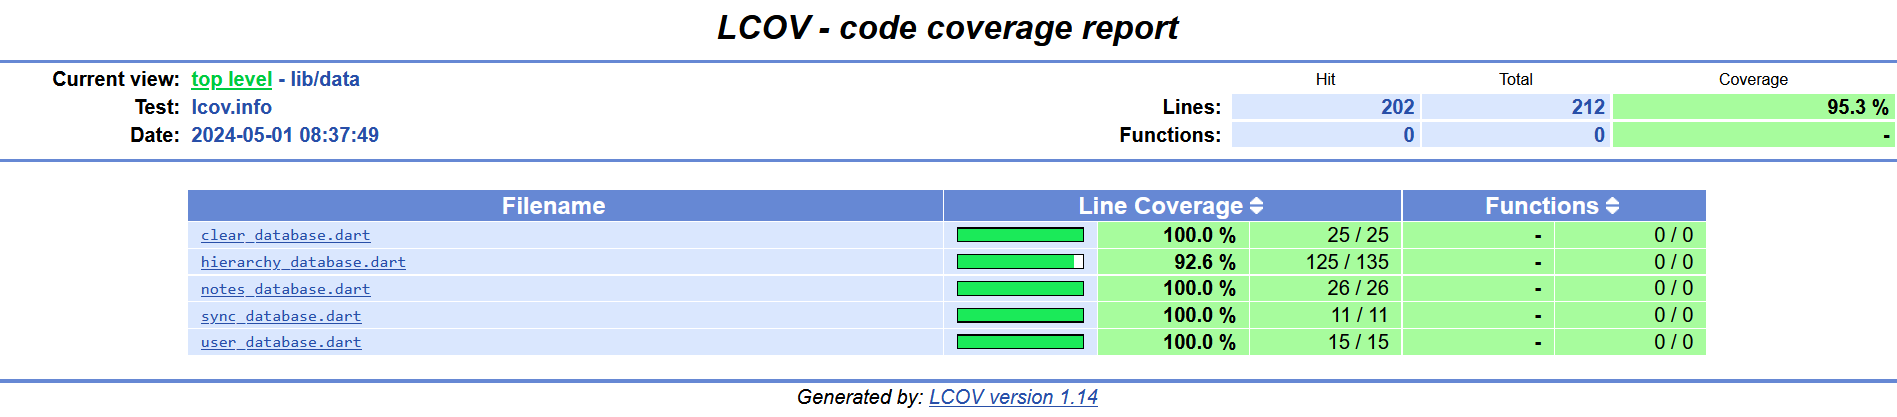
\includegraphics[width=1\textwidth]{img/BP-Runt/Testing/coverage-local-database.png}
  \caption{Statistika pokrytí kódu jednotlivých tříd}
  \label{fig:coverage-report}
\end{figure}

Při vývoji Flutter aplikací lze pokrytí kódu zjistit příkazem \texttt{flutter test --coverage}. Tento příkaz provede všechny automatické testy a vygeneruje soubor \texttt{lcov.info}, umístěný v adresáři \texttt{coverage/}, který obsahuje informace o pokrytí ve formátu \gls{LCOV}. V operačních systémech Linux a Mac pak lze z vygenerovaného souboru \texttt{lcov.info} pomocí \texttt{genhtml} vygenerovat \gls{HTML} stránku, která přehledně zobrazuje, jak velké procento jednotlivých řádků bylo otestováno viz obrázek \ref{fig:coverage-report}. Při rozkliknutí konkrétní třídy jsou světle modrou barvou zvýrazněny řádky, které byly otestovány. Řádky, které nebyly otestovány, jsou zvýrazněny oranžově viz obrázek \ref{fig:line-coverage}. 

\begin{figure}[h!]
  \centering
  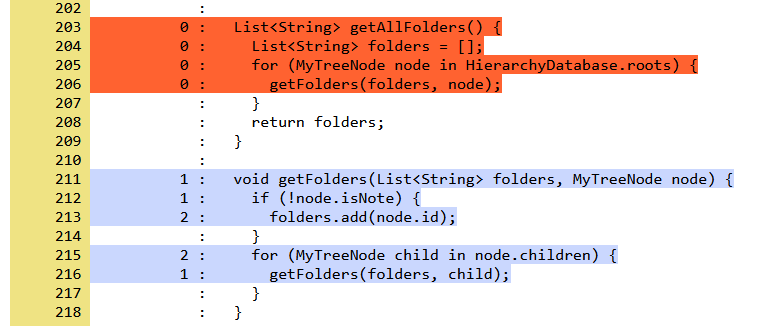
\includegraphics[width=0.9\textwidth]{img/BP-Runt/Testing/line-coverage.PNG}
  \caption{Označení otestovaných a neotestovaných řádek kódu}
  \label{fig:line-coverage}
\end{figure}

\newpage

\section{Manuální testování}

Automatické testy dokážou rychle a opakovaně otestovat velkou část kódu, nezaručují však, že je otestovaný kód bezchybný. Některé aspekty programu se navíc testují automaticky velice obtížně. Proto naší aplikaci prověříme několika testovacími scénáři, při kterých si budeme všímat reakcí a vzhledu systému.

Jelikož se aplikace může chovat odlišně na různých zařízeních. Otestujeme aplikaci na množině mobilních zařízení, emulátorech i v několika webových prohlížečích, abychom si byli jisti, že aplikace bude bez problému fungovat na většině zařízení. 

\subsection{Zařízení}

Pro manuální testování byla aplikace otestována na několika mobilních zařízeních a~emulátorech s různou verzí Androidu. Podrobný přehled zařízení je dostupný v~tabulce \ref{tab:devices}. Abychom si byli jisti s funkčností webové verze aplikace, otestovali jsme webovou verzi aplikace v prohlížečích Google Chrome, Mozilla Firefox a Microsoft Edge na počítači i mobilním zařízení Xiaomi Redmi Note 7, abychom věděli, že~se~aplikace chová a zobrazuje správně. 


\begin{center}
\begin{longtable}{lccc}
\caption{Seznam zařízení, na kterých byla mobilní verze aplikace testována}
\label{tab:devices}\\
\toprule[1.5pt]
\textbf{Název zařízení} & \textbf{Verze Androidu} & \textbf{Rozlišení} &  \textbf{Typ zařízení}\\
\midrule
\endfirsthead
\multicolumn{2}{c}{\tablename{}~\thetable{}
    \textit{(pokračování z~předchozí stránky)}}\\
\midrule
\textbf{Název zařízení} & \textbf{Verze Androidu} & \textbf{Rozlišení} &  \textbf{Typ zařízení}\\
\midrule
\endhead
\midrule
\multicolumn{2}{r}{%
    \textit{(tabulka pokračuje na další stránce)}}\\
\endfoot
\bottomrule[1.5pt]
\endlastfoot
Pixel 3a & 14 (\gls{API} 34) & 1080x2220 & virtuální \\ \hline
Pixel 8 Pro & 14 (\gls{API} 34) & 1344x2992 & virtuální \\ \hline
Pixel Fold & 11 (\gls{API} 30) & 1840x2208 & virtuální\\ \hline
Redmi Note 7 & 10 (\gls{API} 29) & 2340x1080 & fyzické \\ \hline
Redmi Note 11 & 13 (\gls{API} 33) & 2400x1080 & fyzické \\ \hline
\end{longtable}
\end{center}

\subsection{Testovací scénáře}

Následujícími testovacími scénáři byla ověřena základní funkcionalita aplikace:

\vspace{0.1cm}

%------------------------ Vytvoření hiearachie -----------------------------------------------

\noindent \textbf{Vytvoření hierarchie a editace poznámky}

\vspace{0.1cm}

\noindent \textbf{Popis:} Cílem tohoto testu je otestovat, zda lze vytvořit hierarchickou strukturu. V~hierarchické struktuře bude následně vytvořena poznámka, ve které bude napsán formátovaný text. Následně bude zkontrolováno, zda jsou data aplikace uchována i~po zavření aplikace. Jedinou prerekvizitou pro tento test je česká lokalizace aplikace.

\newpage

\noindent \textbf{Postup:}

\begin{enumerate}[label=\arabic*., itemsep=0pt, topsep=0pt, parsep=0pt]
    \item Zobrazíme vysouvací menu a stiskneme tlačítko \textit{Nová složka}. Po stisknutí tlačítka by se mělo zobrazit dialogové okno s titulkem \textit{Nová složka}.
    \item Zadáme do textového pole text \textit{Škola} a stiskneme tlačítko \textit{Vytvořit}. Výsledkem by měla být nově vytvořená složka v hierarchickém stromě.
    \item Stiskneme tři tečky na konci řádku složky. Mělo by se zobrazit menu obsahující položky \textit{Smazat}, \textit{Přejmenovat}, \textit{Nová poznámka}, \textit{Nová složka}, \textit{Přesunout}.
    \item Stiskneme položku v~menu s názvem \textit{Nová složka} a obdobným způsobem jako v~bodě 1 vytvoříme složku s názvem \textit{UPS}. V hierarchickém stromě by se~měla zobrazit složka s~názvem \textit{UPS}, která je potomkem složky \textit{Škola}.
    \item Klikneme na název složky \textit{UPS}. Měla by se zobrazit obrazovka s tlačítkem o~úroveň výš a textový řetězec \textit{Tato složka je prázdná}. V horní liště by měla být zobrazena aktuální cesta \textit{|Škola|UPS}.
    \item Stiskneme plovoucí tlačítko v pravém dolním rohu obrazovky a zvolíme možnost \textit{Nová poznámka} (ikona článku). Objeví se dialogové okno, do kterého zadáme text \textit{Přednáška 1} a stiskneme tlačítko \textit{Vytvořit}. Dialogové okno by se~po~stisknutí tlačítka mělo zavřít a v seznamu by se měla objevit poznámka s~názvem \textit{Přednáška 1}.
    \item Stiskneme položku seznamu \textit{Přednáška 1}. Měli bychom být přesměrováni do~editoru formátovaného textu.
    \item Zadáme libovolný text a aplikaci zavřeme.
    \item Spustíme aplikaci a otevřeme vysouvací menu. Ve stromové struktuře bychom měli najít poznámku \textit{Přednáška 1}.
    \item Otevřeme poznámku kliknutím na jméno poznámky a zkontrolujeme, zda obsah poznámky souhlasí s tím, co jsme napsali před zavřením aplikace.
\end{enumerate}

\noindent \textbf{Výsledek testu:} V rámci testu bylo zjištěno, že při tvorbě kořenového adresáře se tento soubor vytvořil, avšak stromová struktura tento soubor nezobrazovala. Při vytváření podřízených souborů a editace poznámky nebyly nalezeny žádné chyby. 

\vspace{0.1cm}

%------------------------ Úprava poznámky ----------------------------------------------

\noindent \textbf{Úprava a smazání poznámky}

\vspace{0.1cm}

\noindent \textbf{Popis:} Cílem testu je otestovat, zda lze poznámku přejmenovat a přesunout bez ztráty dat. Na konci testu se pokusíme poznámku smazat. Prerekvizitou testu je hierarchie vytvořena v předešlém testu.

\vspace{0.1cm}

\noindent \textbf{Postup:}

\begin{enumerate}[label=\arabic*., itemsep=0pt, topsep=0pt, parsep=0pt]
    \item Otevřeme vysouvací menu a v hierarchickém stromě najdeme poznámku s názvem \textit{Přednáška 1}.
    \item Zmáčkneme tři tečky na konci řádku. Zobrazí se dialogové okno s titulkem \textit{Přejmenovat Přednáška 1}. Do dialogového okna zadáme nový název \textit{Poznámka} a stiskneme tlačítko \textit{Přejmenovat}. Dialogové okno by se mělo zavřít a ve stromě by se mělo změnit jméno souboru.
    \item Stiskneme tlačítko pro vytvoření nové složky a vytvoříme novou složku, kterou pojmenujeme \textit{Práce}.
    \item Stiskneme tři tečky u poznámky, která byla přejmenována v prvním kroku, a~v~menu zvolíme možnost \textit{Přesunout}. Zobrazí se dialogové okno s rozbalovacím seznamem, ve kterém by se měly nacházet 2 položky: \textit{|Škola} a \textit{|Práce}. Zvolíme možnost \textit{|Práce}. Dialogové okno by se mělo uzavřít a poznámka by měla být přesunuta do složky \textit{Práce}.
    \item Přesunutou poznámku otevřeme a zkontrolujeme, zda se obsah této poznámky nezměnil.
    \item Otevřeme vysouvací menu, stiskneme tři tečky u poznámky a stiskneme volbu \textit{Smazat}. Mělo by se zobrazit potvrzovací dialogové okno.
    \item V dialogovém okně stiskneme tlačítko \textit{Smazat}. Dialogové okno by se mělo zavřít a poznámka by měla být odebrána ze stromové struktury. 
\end{enumerate}

\noindent \textbf{Výsledek testu:} Během testu došlo k přejmenování, přesunutí a smazání poznámky. Nebyly nalezeny žádné chyby.

%------------------------ Registrace uživatele ----------------------------------------------

\noindent \textbf{Registrace uživatele}

\noindent \textbf{Popis:} V tomto testovacím scénáři ověříme, že uživateli je umožněno založit si~nový účet. Současně zkusíme některé chybové stavy, které mohou při registraci nastat. Prerekvizitou je nastavení české lokalizace, stabilní internetové připojení, nepřihlášený uživatel a neexistující účet \textit{test@gmail.com}.

\noindent \textbf{Postup:}

\begin{enumerate}[label=\arabic*., itemsep=0pt, topsep=0pt, parsep=0pt]
    \item Otevřeme vysouvací menu a klikneme na tlačítko \textit{Registrovat}. Po této akci bychom měli být přesměrováni na obrazovku registrace.
    \item Nevyplníme žádné textové pole a stiskneme tlačítko \textit{Registrovat}. Mělo by se~zobrazit chybové hlášení: \textit{Jedno nebo více textových polí je prázdné!}
    \item Do textového pole pro e-mailovou adresu zadáme \textit{test@gmail.com}, do textového pole určeného pro heslo zadáme textový řetězec \textit{heslo}, do textového pole pro ověření hesla zadáme \textit{Heslo123} a stiskneme tlačítko \textit{Registrovat}. Výsledkem bude chybové oznámení: \textit{Hesla se neshodují!}
    \item Do obou textových polí pro zadání hesla zadáme \textit{heslo} a stiskneme tlačítko pro registraci. Výsledkem bude chybové oznámení: \textit{Heslo je příliš krátké. Heslo musí obsahovat nejméně 6 znaků!}
    \item Do obou textových polí pro zadání hesla zadáme \textit{Heslo123}, obsah textového pole e-mailu změníme na \textit{test} a stiskneme tlačítko \textit{Registrovat}. Výsledkem bude chybové oznámení: \textit{Špatný formát e-mailové adresy!}
    \item Změníme opět e-mailovou na původní hodnotu \textit{test@gmail.com} a stiskneme tlačítko \textit{Registrovat}. Mělo by se zobrazit načítání. Po krátké době bychom měli být přesměrováni na obrazovku s otevřeným vysouvacím menu. V hlavičce vysouvacího menu by se mělo zobrazit: \textit{Přihlášený uživatel: test@gmail.com} a~tlačítko \textit{Odhlásit}.
\end{enumerate}

\noindent \textbf{Výsledek testu:} V rámci testování byla ověřena funkce registrace nového uživatele. Program se choval dle uvedeného popisu.

\vspace{0.1cm}

%------------------------ Registrace emailem a heslem ----------------------------------------

\noindent \textbf{Přihlášení e-mailem a heslem}

\vspace{0.1cm}

\noindent \textbf{Popis:} V tomto testu ověříme, že uživatel je schopen se přihlásit ke svému existujícímu účtu. Prerekvizitou testovacího scénáře je nastavení české lokalizace, nepřihlášený uživatel, stabilní internetové připojení, neexistující účet \textit{notexist@gmail.com} a~existující účet \textit{test@gmail.com} s heslem \textit{Heslo123}.

\vspace{0.1cm}

\noindent \textbf{Postup:}

\begin{enumerate}[label=\arabic*., itemsep=0pt, topsep=0pt, parsep=0pt]
    \item Otevřeme vysouvací menu a klikneme na tlačítko \textit{Přihlásit}. Po této akci bychom měli být přesměrováni na obrazovku přihlášení.
    \item Nevyplníme žádné textové pole a stiskneme tlačítko \textit{Přihlásit}. Mělo by se~zobrazit chybové hlášení: \textit{Jedno nebo více textových polí je prázdné!}
    \item Do prvního textového pole zadáme e-mailovou adresu \textit{test@gmail.com} a stiskneme tlačítko \textit{Přihlásit}. Výsledkem bude chybové oznámení: \textit{Špatná e-mailová adresa nebo heslo!}
    \item Do textového pole hesla zadáme textový řetězec \textit{Heslo123} a stiskneme tlačítko \textit{Přihlásit}. Měli bychom vidět indikátor načítání a následně bychom měli být přesměrováni na obrazovku s otevřeným vysouvacím menu. V hlavičce vysouvacího menu by se mělo zobrazit: \textit{Přihlášený uživatel: test@gmail.com} a tlačítko \text{Odhlásit}. Data, která byla uložena na účtu by měla být uložena a~zobrazena v~aplikaci. 
\end{enumerate}

\noindent \textbf{Výsledek testu:} Během testování došlo k přihlášení k existujícímu účtu. Uživatelská data byla uložena. Test byl úspěšný.

\vspace{0.1cm}

%------------------------ Přihlášení Google účtem -------------------------------------------

\noindent \textbf{Přihlášení účtem Google}

\vspace{0.1cm}

\noindent \textbf{Popis:} V tomto testovacím scénáři ověříme, zda je uživatel schopen se přihlásit pomocí účtu Google. Prerekvizitou testovacího scénáře je nastavení české lokalizace, nepřihlášený uživatel, stabilní internetové připojení, existující Google účet, ke~kterému má tester přístup.

\vspace{0.1cm}

\noindent \textbf{Postup:}

\begin{enumerate}[label=\arabic*., itemsep=0pt, topsep=0pt, parsep=0pt]
    \item Otevřeme vysouvací menu a klikneme na tlačítko \textit{Přihlásit}. Po této akci bychom měli být přesměrováni na obrazovku přihlášení.
    \item Klikneme na ikonu Google ve spodní části obrazovky. Po stisknutí by se mělo zobrazit přihlašovací okno pro přihlášení Google účtem.
    \item Zvolíme svůj Google účet. Aplikace by nás měla přihlásit a přesměrovat zpět na vysouvací menu. Zároveň stáhnout uložená data, která jsou na cloudu uložena.
\end{enumerate}

\noindent \textbf{Výsledek testu:} Ve webové verzi aplikace byla nalezena chyba při přihlášení účtem Google. V mobilní verzi aplikace bylo přihlašování účtem Google úspěšné.

\newpage

%------------------------ Odhlášení uživatele -----------------------------------------------

\noindent \textbf{Odhlášení přihlášeného uživatele}

\vspace{0.1cm}

\noindent \textbf{Popis:} V tomto testu se ověříme funkcionalitu odhlášení. Prerekvizitou je přihlášený uživatel a data vytvořená v testovacím scénáři: Vytvoření hierarchie a editace poznámky. 

\vspace{0.1cm}

\noindent \textbf{Postup:}

\begin{enumerate}[label=\arabic*., itemsep=0pt, topsep=0pt, parsep=0pt]
    \item Zobrazíme vysouvací menu. V hlavičce vysouvacího menu by měl být text \textit{Přihlášený uživatel} s e-mailovou adresou přihlášeného uživatele. Pod textem by se mělo nacházet tlačítko \textit{Odhlásit}. V hierarchickém stromě by se měla nacházet uložená data.
    \item Stiskneme tlačítko \textit{Odhlásit}. Hlavička vysouvacího menu by měla změnit svůj obsah na text \textit{Nepřihlášený uživatel} a zobrazit tlačítka \textit{Přihlásit} a \textit{Registrovat}. Všechna data v hierarchickém stromě by měla být smazána.
\end{enumerate}

\noindent \textbf{Výsledek testu:} Uživatel byl úspěšně odhlášen a data byla smazána.

\vspace{0.1cm}

%------------------------ Změna hesla -------------------------------------------------------

\noindent \textbf{Změna zapomenutého hesla}

\vspace{0.1cm}

\noindent \textbf{Popis:} V tomto testu ověříme, zda je uživatel schopen změnit si heslo, pokud jej zapomene. Prerekvizitou testovacího scénáře je nastavení české lokalizace, nepřihlášený uživatel, existující účet \textit{lrunt@students.zcu.cz} (nebo jiný, ke kterému má tester přístup) a otevřená obrazovka pro přihlášení uživatele.

\vspace{0.1cm}

\noindent \textbf{Postup:}

\begin{enumerate}[label=\arabic*., itemsep=0pt, topsep=0pt, parsep=0pt]
    \item Na obrazovce pro přihlášení uživatele stiskneme odkaz \textit{Obnovit heslo}. Měli bychom být přesměrováni na stránku pro zaslání e-mailu s odkazem pro obnovu hesla s jedním textovým polem a jedním tlačítkem.
    \item Do textového pole zadáme e-mailovou adresu \textit{lrunt@students.zcu.cz} a stiskneme tlačítko \textit{Odeslat e-mail}. Výsledkem bude zobrazený Toast s textem \textit{E-mail pro obnovení hesla byl odeslán} a přesměrování na obrazovku pro přihlášení uživatele. 
    \item Zkontrolujeme e-mailovou schránku. Měl by nám přijít e-mail s předmětem \textit{Reset your password for Notes} a odkazem na stránku pro změnu hesla (odesílání e-mailu může trvat několik minut). 
    \item Otevřeme hypertextový odkaz, který nám přišel v e-mailu. Měli bychom být přesměrováni na stránku pro změnu hesla. Do textového pole na otevřené stránce zadáme textový řetězec \textit{password} a stiskneme tlačítko \textit{Save}.
    \item Nyní se zkusíme v aplikaci Notes přihlásit s novými přihlašovacími údaji e-mailem \textit{lrunt@students.zcu.cz} a heslem \textit{password}. Měli bychom být přihlášeni a~přesunuti na obrazovku s otevřeným vysouvacím menu.
\end{enumerate}

\noindent \textbf{Výsledek testu:} Odesílání e-mailu ve většině případů trvalo trochu déle. Heslo bylo ve všech případech změněno dle předpokladů.

\vspace{0.1cm}

%------------------------ Synchronizace bez konfliktů --------------------------------------
\newpage

\noindent \textbf{Synchronizace dat bez konfliktu}

\vspace{0.1cm}

\noindent \textbf{Popis:} Tento testovací scénář testuje, že je aplikace schopna synchronizovat uživatelská data bez vyvolaných konfliktů. Prerekvizitou jsou dvě zařízení, na kterých je aplikace spuštěna, přihlášení na obou zařízení ke stejnému účtu.  

\vspace{0.1cm}

\noindent \textbf{Postup:}

\begin{enumerate}[label=\arabic*., itemsep=0pt, topsep=0pt, parsep=0pt]
    \item Na zařízení 1 vytvoříme složku, kterou nazveme \textit{Synchronizace} a stiskneme tlačítko \textit{Synchronizace}.
    \item Na zařízení 2 stiskneme tlačítko \textit{Synchronizace}. Složka se jménem \textit{Synchronizace} by se měla zobrazit v hierarchickém stromě.
    \item Na zařízení 2 vytvoříme ve složce \textit{Synchronizace} poznámku s libovolným jménem. Poznámku otevřeme a zadáme libovolný text. Po úpravě stiskneme tlačítko \textit{Synchronizace}.
    \item Na zařízení 1 stiskneme tlačítko \textit{Synchronizace} a zkontrolujeme správnost synchronizovaných dat.
\end{enumerate}

\noindent \textbf{Výsledek testu:} Během testování nebyly objeveny žádné chyby. Data byla bez problémů synchronizována.

\vspace{0.1cm}

%------------------------ Synchronizace s konfliky--------------------------------------

\noindent \textbf{Synchronizace dat s vyvoláním konfliktů}

\vspace{0.1cm}

\noindent \textbf{Popis:} Tento testovací scénář testuje detekci a řešení konfliktů. Prerekvizitami jsou dvě zařízení, na kterých je aplikace spuštěna, přihlášení na obou zařízeních ke stejnému účtu a nějaká počáteční data.  

\vspace{0.1cm}

\noindent \textbf{Postup:}

\begin{enumerate}[label=\arabic*., itemsep=0pt, topsep=0pt, parsep=0pt]
    \item Na zařízení 1 vytvoříme složku s libovolným jménem a stiskneme tlačítko \textit{Synchronizace}.
    \item Na zařízení 2 stiskneme tlačítko \textit{Synchronizace}. Složka se jménem \textit{Synchronizace} by se měla zobrazit v hierarchickém stromě.
    \item Na zařízení 2 v námi vytvořené složce vytvoříme poznámku libovolně pojmenovanou poznámku. Poznámku otevřeme a zadáme libovolný text. Tím na zařízení 2 skončíme.
    \item Na zařízení 1 vytváříme v námi vytvořené složce poznámku, definujeme její obsah a stiskneme tlačítko \textit{Synchronizace}.
    \item Na zařízení 2 stiskneme tlačítko \textit{Synchronizace}. Měl by se objevit Toast s~textem, že se byly detekovány konflikty. V hierarchickém stromě by se~měl objevit obsah zařízení 1.
    \item Na zařízení 2 otevřeme nastavení a stiskneme možnost \textit{Konflikty}. V konfliktech by měla být uložena námi vytvořená struktura s časovou značkou, kdy byla synchronizace provedena.
    \item Stiskneme tři tečky na konci řádku a zkusíme tento konflikt smazat. Konflikt by měl být smazán.
\end{enumerate}

\noindent \textbf{Výsledek testu:} Během testu byl detekován konflikt dat a data byla uložena na~očekávaném místě s časovou značkou. Smazání konfliktních dat proběhlo taktéž bez problémů. 

\vspace{0.1cm}

%------------------------ Lokalizace -----------------------------------------------

\noindent \textbf{Změna lokalizace}

\vspace{0.1cm}

\noindent \textbf{Popis:} V tomto testu zkontrolujeme, zda se všechny texty správně překládají. Testovací scénář nemá žádné prerekvizity.

\vspace{0.1cm}

\noindent \textbf{Postup:}

\begin{enumerate}[label=\arabic*., itemsep=0pt, topsep=0pt, parsep=0pt]
    \item Zkoušíme procházet všechny obrazovky a dialogová okna aplikace. Všímáme si, zda jsou všechny texty ve správném jazyce.
    \item Otevřeme menu aplikace (Ozubené kolo v pravém horním rohu).
    \item V poli Jazyk zvolíme druhý jazyk.
    \item Opět procházíme celou aplikaci a sledujeme, zda jsou všechny textové řetězce ve správném jazyce.
\end{enumerate}

\noindent \textbf{Výsledek testu:} V aplikaci bylo nalezeno pár řetězců, které byly buď umístěny špatně (například \textit{název poznámky} v dialogovém okně pro založení adresáře), nebo neexistoval jejich překlad. 

\vspace{0.1cm}

%------------------------ Tmavý mód -----------------------------------------------

\noindent \textbf{Změna barevného módu}

\vspace{0.1cm}

\noindent \textbf{Popis:} V tomto testu ověříme správný vzhled a přepínání témat. Testovací scénář nemá žádné prerekvizity.

\vspace{0.1cm}

\noindent \textbf{Postup:}

\begin{enumerate}[label=\arabic*., itemsep=0pt, topsep=0pt, parsep=0pt]
    \item Zkoušíme procházet všechny obrazovky a dialogová okna aplikace. Všímáme si, zda všechny komponenty mají správnou barvu a správné rozložení.
    \item Otevřeme menu aplikace (Ozubené kolo v pravém horním rohu).
    \item V poli Tmavý mód stiskneme přepínač, kterým by se mělo změnit téma aplikace.
    \item Procházíme celou aplikaci a kontrolujeme, zda všechny komponenty odpovídají aktuálně zvolenému barevnému tématu.
\end{enumerate}

\noindent \textbf{Výsledek testu:} V rámci testu byl zkontrolován vzhled aplikace. Rozložení a velikost některých komponent (například rozložení tlačítek \textit{Přihlásit} a \textit{Registrovat} ve~vysouvacím menu) bylo změněno. 

\newpage

\section{Hodnocení kvality aplikace}

V při vývoji je vhodné vyhodnotit kvalitu vytvářené aplikace. Kvalita aplikací většinou ovlivňuje uživatelskou spokojenost a funkčnost aplikace. Normy „Core App Quality"\footnote{https://developer.android.com/docs/quality-guidelines/core-app-quality} poskytované společností Google definují kritéria pro hodnocení aplikací. Tyto standardy umožňují systematicky vyhodnotit kvalitu aplikace.

\begin{center}
\begin{longtable}{p{0.4\textwidth} p{0.5\textwidth}}
\caption{Kritéria „Core App Quality", které aplikace splňuje}
\label{tab:kriteria}\\
\toprule[1.5pt]
\textbf{Kategorie} & \textbf{ID splněného kritéria}\\
\midrule
\endfirsthead
\multicolumn{2}{c}{\tablename{}~\thetable{}
    \textit{(pokračování z~předchozí stránky)}}\\
\midrule
\textbf{Kategorie} & \textbf{ID splněného kritéria}\\
\midrule
\endhead
\midrule
\multicolumn{2}{r}{%
    \textit{(tabulka pokračuje na další stránce)}}\\
\endfoot
\bottomrule[1.5pt]
\endlastfoot
Vizuální zážitek & VX-N1, VX-N2, VX-N3, VX-S1, VX-S2, VX-V1,
VX-V2, VX-V3, VX-A1, VX-A2 \\ \hline
Funkcionalita & FN-B1 \\ \hline
Výkon a stabilita & PS-S1, PS-P1, PS-T1, PS-T2, PS-T5, PS-T6 \\ \hline
Ochrana soukromí a zabezpečení & SC-P1, SC-P2, SC-P3, SC-P4, SC-DF1, SC-DF2, SC-DF3, SC-N1, SC-C1 \\ \hline
\end{longtable}
\end{center}

V tabulce \ref{tab:kriteria} jsou uvedena kritéria, která vyvíjená aplikace splňuje. Tato kritéria jsou rozdělena dle kategorií. Kritérium VX-V3 v kategorii vizuální zážitek například znamená, že aplikace a veškerý webový obsah, na který aplikace odkazuje, podporuje tmavý režim.  

% _____________________________________________________________________________
%
%
%        CHAPTER Possible extensions
%
% _____________________________________________________________________________
%
\chapter{Možná rozšíření}

 Od začátku vývoje se aplikace vytvářela se snahou na bezproblémové přidání dalších funkcí. V následující kapitole jsou popsány možná rozšíření již námi vytvořené aplikace. Jedná se o rozšíření zavádějící novou funkcionalitu, zlepšující komfort uživatelů a rozšíření podpory na více platforem.

\section{Spolupráce více uživatelů}

V současné verzi aplikace může uživatel synchronizovat poznámky mezi svými zařízeními v rámci svého účtu. Někdy je však potřeba sdílet poznámky s více uživateli nebo spolupracovat v týmu. Dalším rozšířením by mohlo být sdílení a spolupráce více uživatelů na jedné poznámce. Uživatelé by měli možnost sdílet libovolný soubor s dalším uživatelem, kterému by mohli přidávat a odebírat oprávnění, jak může s daným souborem zacházet.

Pro tuto funkci by bylo potřeba rozšířit datový model informacemi obsahující data o sdílení poznámek. Každý uživatel by mohl mít ve své kolekci informace o~souborech a poznámkách, které jsou s ním sdíleny. V klientovi by byla přidána do~menu položka sdílet s uživatelem, která by zobrazovala dialog s nastavením práv a uživatelem, se kterým by byly poznámky sdíleny. V tomto kroku by se muselo kontrolovat, zda už poznámka není s uživatelem sdílena, aby nedošlo k duplikaci informací. 

\section{Obsah poznámek}

Aktuální verze aplikace poskytuje ukládání poznámek ve formě formátovaného textu, což by některým uživatelům nemuselo stačit. Dalším krokem by tedy mohlo být rozšíření typů obsahu. Kromě textu by aplikace mohla podporovat ukládání obrázků, videí, audio nahrávek nebo skic. Tato média by mohla být vkládána ze~souborového systému nebo by se příslušné digitální soubory mohli vytvářet přímo v~aplikaci s použitím hardwarového vybavení zařízení.

\section{Historie změn}

Pro zvýšení kontroly nad daty by mohla být zavedena historie změn na daném zařízení, která by uživatelům umožňovala vrátit se k libovolné verzi svých poznámek. Tato funkcionalita by mohla přispět k efektivnějšímu řešení konfliktů.

\section{Rozšíření na více platforem} 

Aplikace je vytvořená s použitím technologie Flutter, která nabízí multiplatfomní vývoj aplikací. Tato technologie umožňuje rozšířit aplikaci na další platformy jako jsou iOS, macOS, Windows, Linux a Google Fuchsia. Pro zveřejnění aplikace na~těchto platformách by bylo nutné udělat specifické úpravy ve vzhledu (například použití Cupertino Design pro iOS, upravení rozložení komponent), konfiguraci služby Firebase a úprava závislostí knihoven. Před zveřejněním by bylo vhodné aplikaci znovu otestovat manuálními testy k ověření správné funkčnosti. 


% _____________________________________________________________________________
%
%
%        CHAPTER Possible extensions
%
% _____________________________________________________________________________
%
\chapter{Závěr}

Cílem této bakalářské práce bylo navrhnout a implementovat mobilní aplikaci pro zařízení Android, která bude umožňovat tvorbu hierarchických poznámek s libovolným počtem úrovní. Další požadovanou vlastností aplikace byla synchronizace dat mezi více zařízeními, bezplatné použití a dobrá rozšířitelnost aplikace. Vzhledem k tomu, že většina dostupných aplikací kombinaci těchto požadavků nesplňuje, rozhodli jsme se k vytvoření vlastní aplikace.

V úvodu práce byl proveden podrobný průzkum existujících aplikací, ve kterém bylo zjištěno, jaké funkce tyto aplikace nabízejí. Z těchto poznatků byly nastíněny funkce, které by měla výsledná aplikace obsahovat. V další části proběhla analýza technologií pro vývoj mobilních aplikací a ukládání dat, na základě kterého byly zvoleny technologie Flutter a Firebase. Po výběru konkrétních technologií byly specifikovány případy použití vytvářené aplikace, které byly zohledněny v následujícím návrhu aplikace. V tomto návrhu byl navržen datový model a uživatelské rozhraní vytvářené aplikace. V další fázi byla navržená aplikace úspěšně realizována.

Vytvořená aplikace je dostupná nejen na mobilních zařízeních s operačním systémem Android, ale také jako progresivní webová aplikace, která je veřejně dostupná. Aplikace umožňuje vytvářet a organizovat poznámky s hierarchickou strukturou. Vytvořené poznámky lze synchronizovat mezi více zařízeními s detekcí potenciálních konfliktů. Mezi další zajímavé funkce a vlastnosti aplikace můžeme zařadit tmavý mód, vícejazyčnou podporu, rozšiřitelnost kódu a bezplatné použití. Pro~podporu uživatelů byla vytvořena webová stránka s návodem, jak aplikaci ovládat. V~závěru práce byla aplikace otestována komplexní sadou testů a byla navržena možná rozšíření.


% _____________________________________________________________________________
%
%
%        BACK MATTER (BIBLIOGRAPHY, LISTS, ...)
%
% _____________________________________________________________________________
%
\glsaddall
%\backmatter
\printglossaries
\printbibliography
\listoffigures
\listoftables
\listoflistings

% _____________________________________________________________________________
%
%
%        APPENDICES
%
% _____________________________________________________________________________
%
\appendix
% _____________________________________________________________________________
%
%
%		APPENDIX CHAPTER
%
% _____________________________________________________________________________
%

\chapter{Uživatelská příručka}\label{app:user-manual}

Tato příloha obsahuje uživatelskou příručku aplikace Notes. Cílem této příručky je poskytnout uživatelům jasné a přehledné informace o tom, jak ovládat aplikaci. Podrobnější návod je dostupný na webové stránce: \url{https://notes-manual.web.app/manual-cz.html}

\section{Spuštění aplikace}

Při spuštění aplikace se zobrazí inicializační obrazovka s logem aplikace viz~obrázek~\ref{fig:SplashScreen}.

\begin{figure}[h!]
  \centering
  
\includegraphics[width=0.35\textwidth]{img/BP-Runt/UserManual/SplashScreen.jpg}
  \caption{Inicializační obrazovka}
  \label{fig:SplashScreen}
\end{figure}

Když je aplikace inicializována, zobrazí se uživateli domovská obrazovka viz~obrázek~\ref{fig:WelcomeScreen}.

\begin{figure}[h!]
  \centering
  
\includegraphics[width=0.58\textwidth]{img/BP-Runt/UserManual/WelcomePage.jpg}
  \caption{Snímek úvodní obrazovky aplikace}
  \label{fig:WelcomeScreen}
\end{figure}

Na obrazovce se nacházejí dvě tlačítka. V levém horním rohu jsou tři vodorovné čáry, které otevírají vysouvací menu popsané v sekci \ref{manual:drawer}. V pravém horním rohu se~nachází ikona ozubeného kola, která otevírá nastavení aplikace. Stránka nastavení je~popsána v~sekci~\ref{manual:settings}.

\section{Vysouvací menu} \label{manual:drawer}

Vysouvací menu zobrazuje stav přihlášení uživatele. Pokud je uživatel přihlášen, nachází se v horní části menu informace o přihlášeném účtu a tlačítko pro odhlášení uživatele. Přihlášenému uživateli se zároveň ve spodní části menu zobrazuje tlačítko pro synchronizaci a čas poslední synchronizace. Nepřihlášení uživatelé mají možnost využít tlačítka \textit{Přihlásit} a \textit{Registrovat}.

Ve vysouvacím menu je kromě stavu uživatele zobrazena také hierarchická struktura ve formě stromové komponenty viz obrázek \ref{fig:AppDrawer}. Kliknutím na ikonu adresáře lze rozbalit nebo skrýt podřízené adresáře a poznámky. Pokud uživatel stiskne název souboru nebo ikonu poznámky, je automaticky přesunut na obrazovku adresáře (viz sekce \ref{manual:listView}) či~poznámky (viz sekce v sekce \ref{manual:note}). Každá složka ve stromové struktuře má na konci řádku tři tečky, které zobrazují menu s možnostmi úpravy poznámky či adresáře.   

\begin{figure}[h!]
  \centering
  \begin{minipage}[h]{0.43\textwidth}
    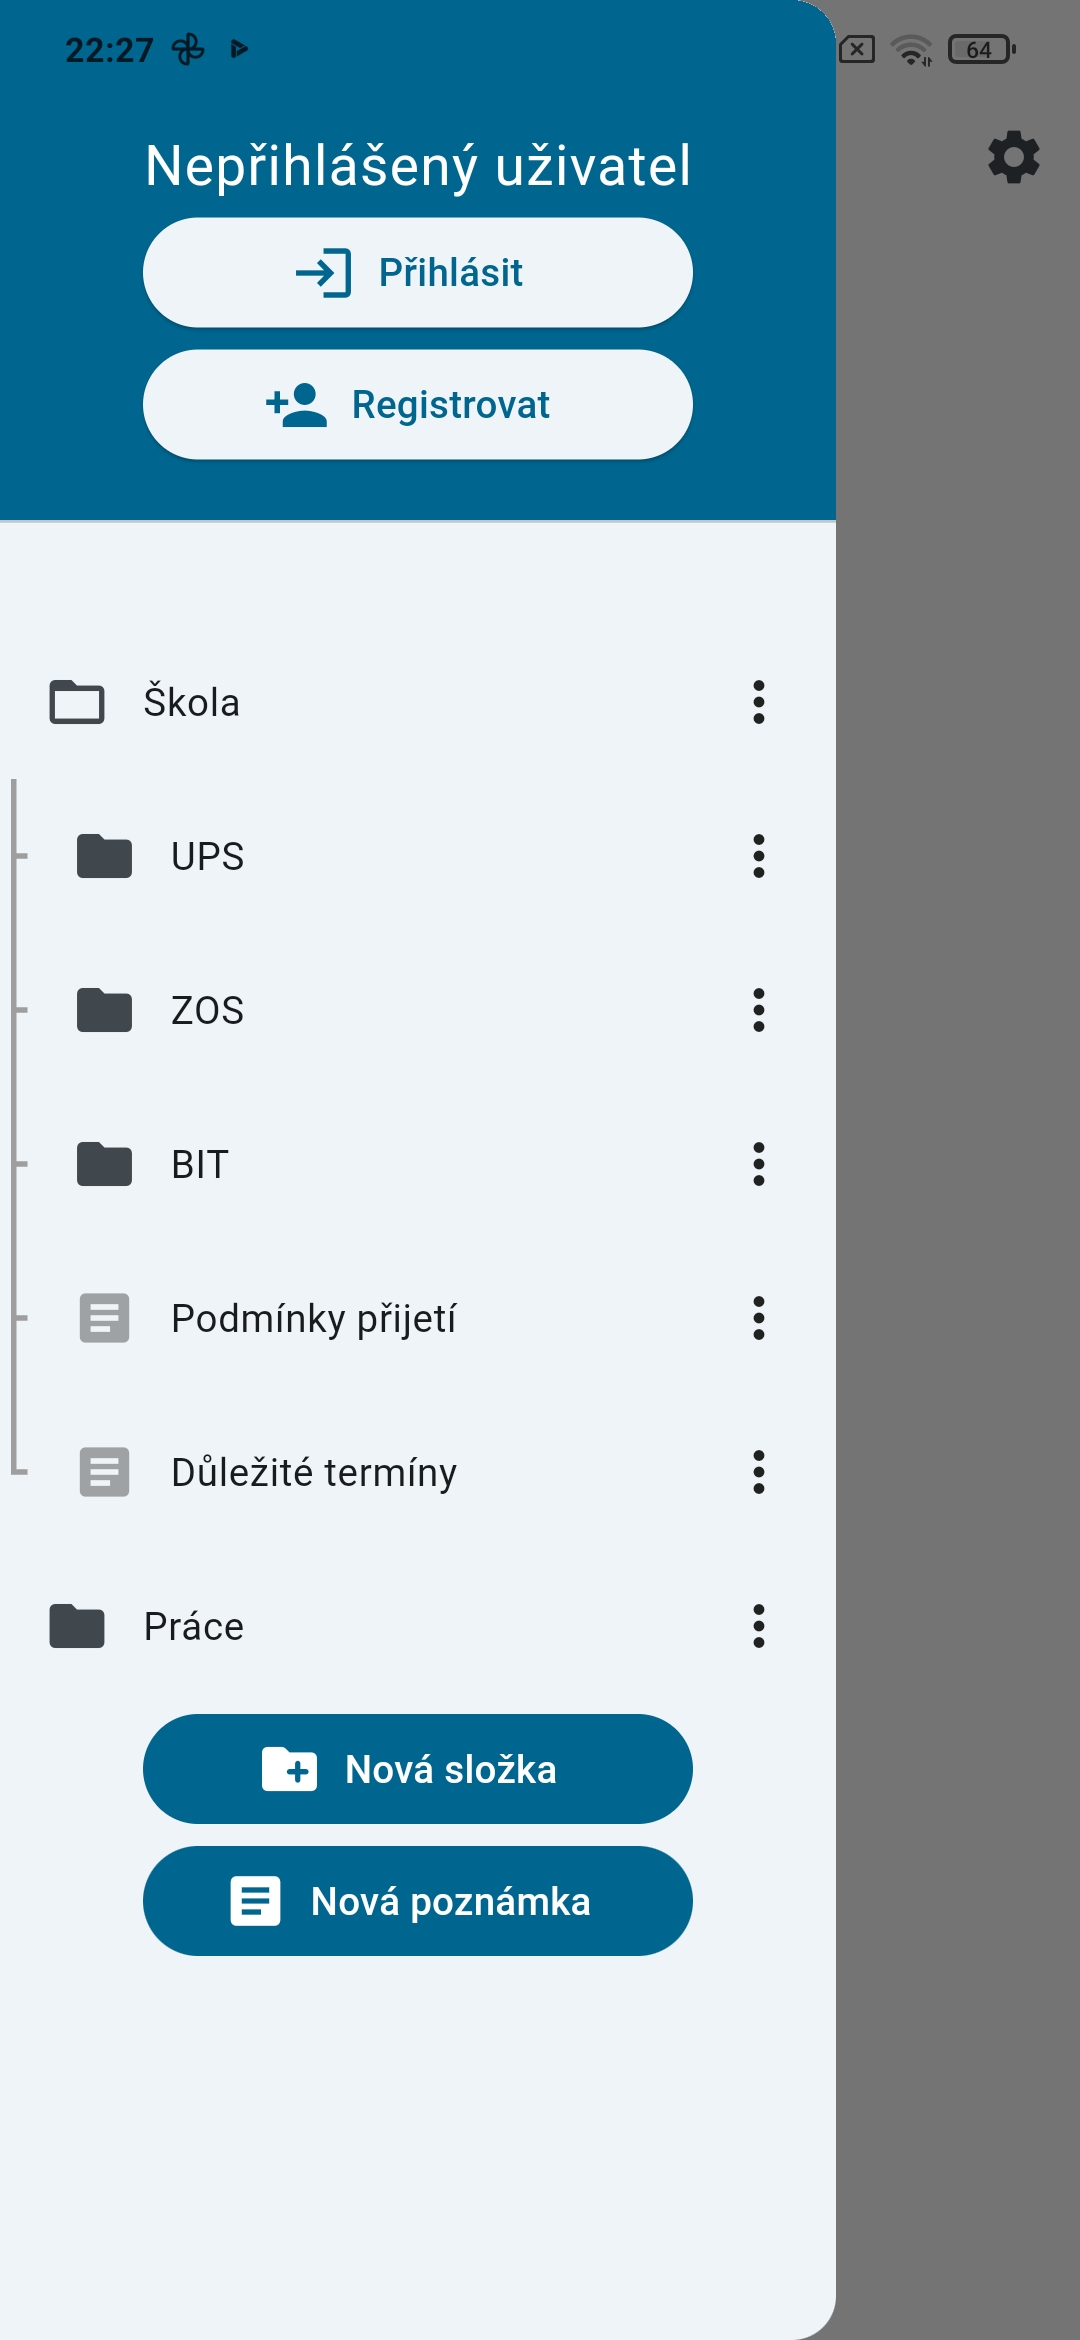
\includegraphics[width=\textwidth]{img/BP-Runt/UserManual/DrawerNotLogged.jpg}
  \end{minipage}
  \hspace{10pt}
  \begin{minipage}[h]{0.43\textwidth}
    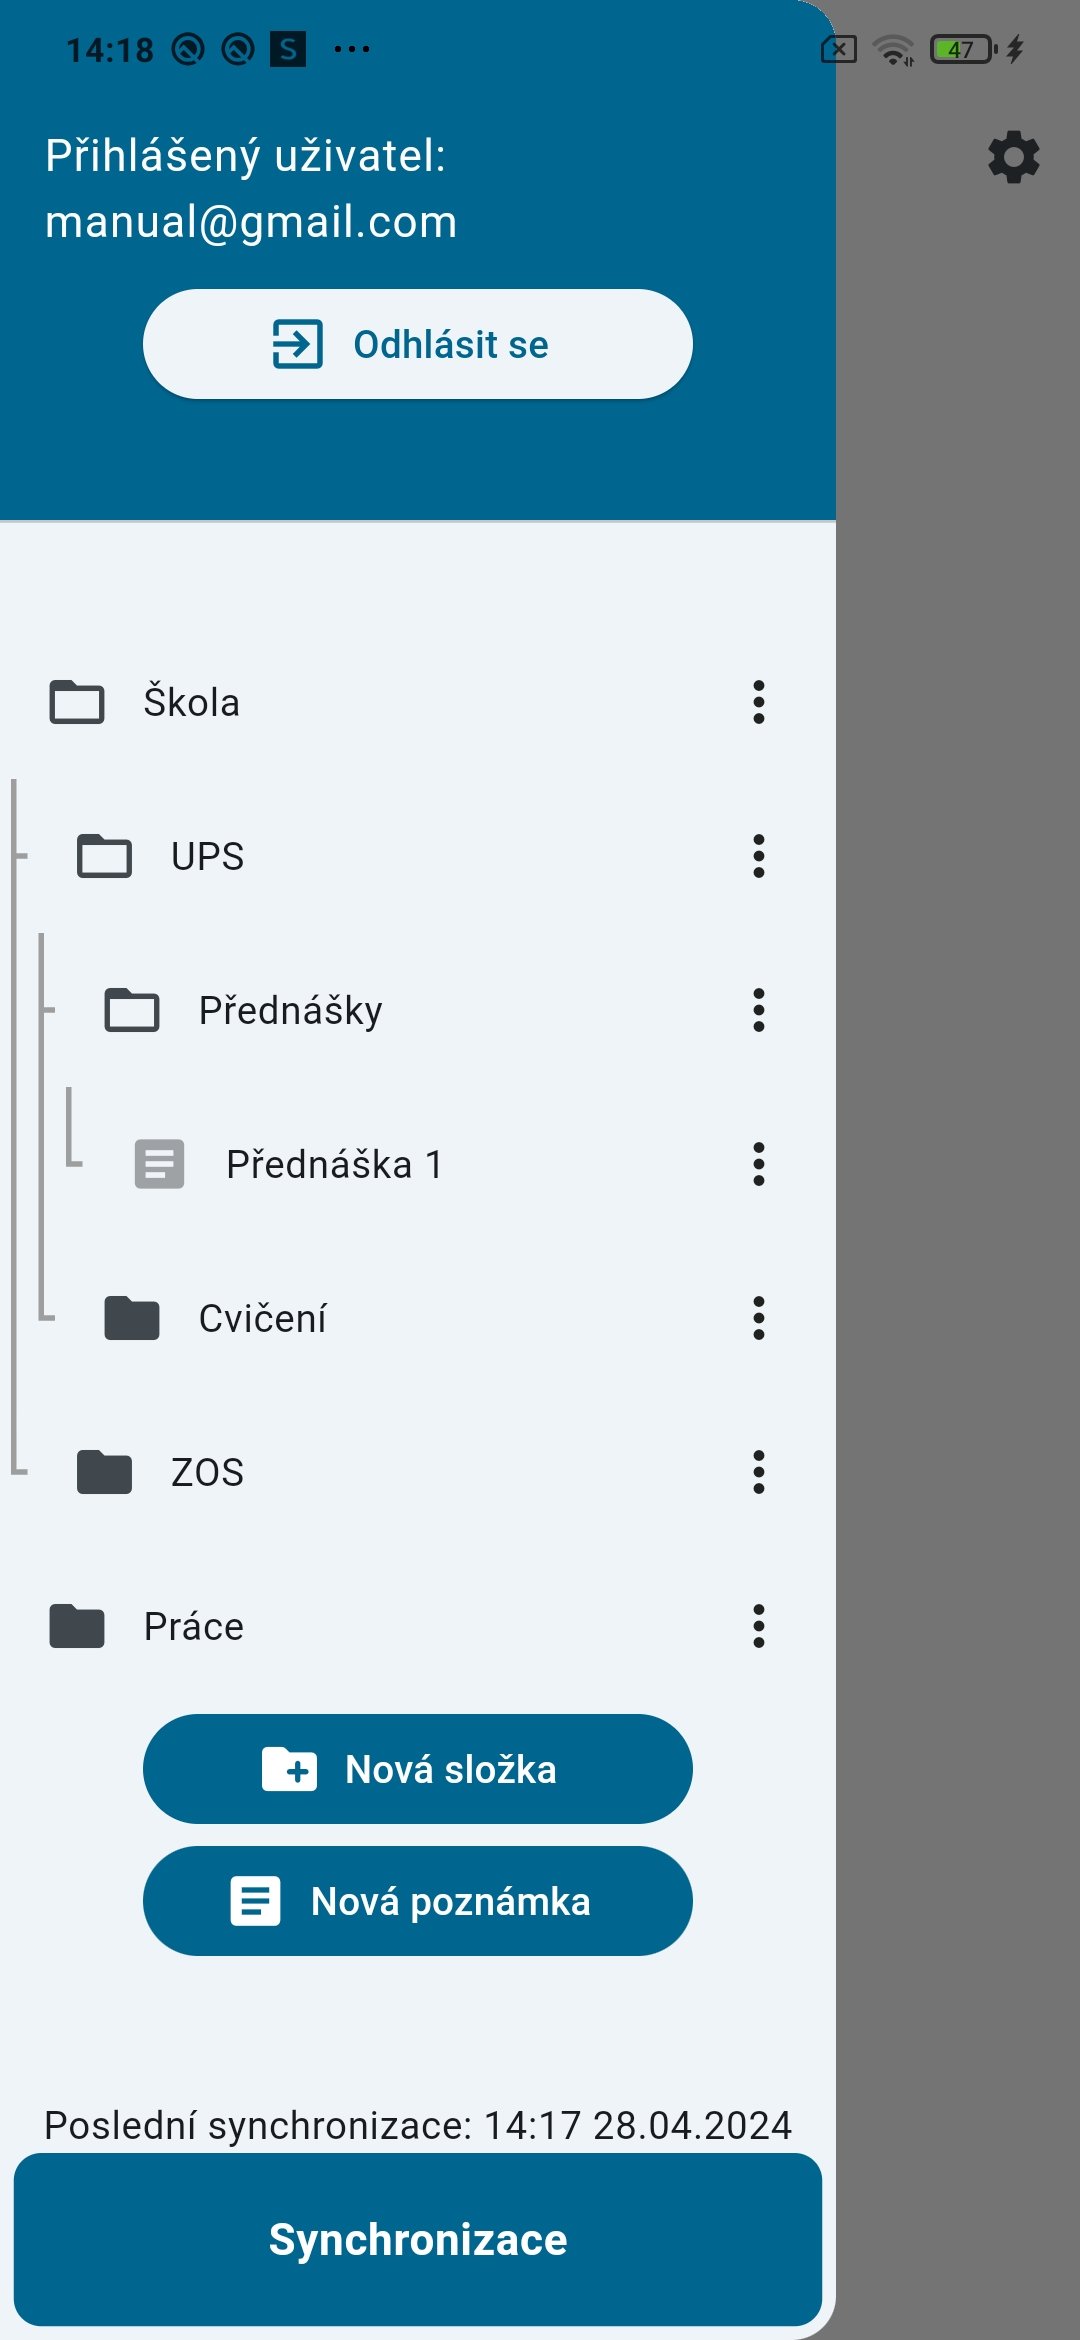
\includegraphics[width=\textwidth]{img/BP-Runt/UserManual/DrawerLoggedUser.jpg}
  \end{minipage}
  \caption{Obrazovky s vysouvacím menu: vlevo vysouvací menu nepřihlášeného uživatele, vpravo vysouvací menu přihlášeného uživatele}
  \label{fig:AppDrawer}
\end{figure}

\section{Obrazovka adresáře} \label{manual:listView}

Na dalším obrázku \ref{fig:FolderScreen} je zobrazena obrazovka s obsahem adresáře. V aplikačním panelu je cesta adresáře, ve kterém se uživatel nachází. Podřízené soubory adresáře jsou zobrazeny v seznamu uprostřed obrazovky. Pokud uživatel stiskne některý ze~souborů, je následně přesměrován do příslušného adresáře či poznámky. V~pravém dolním rohu se nacházejí plovoucí tlačítka, kterými má uživatel možnost vytvářet nové adresáře a poznámky v aktuálním adresáři. Červené tlačítko s křížkem slouží ke skrytí plovoucích tlačítek nad ním. 

\begin{figure}[h!]
  \centering
  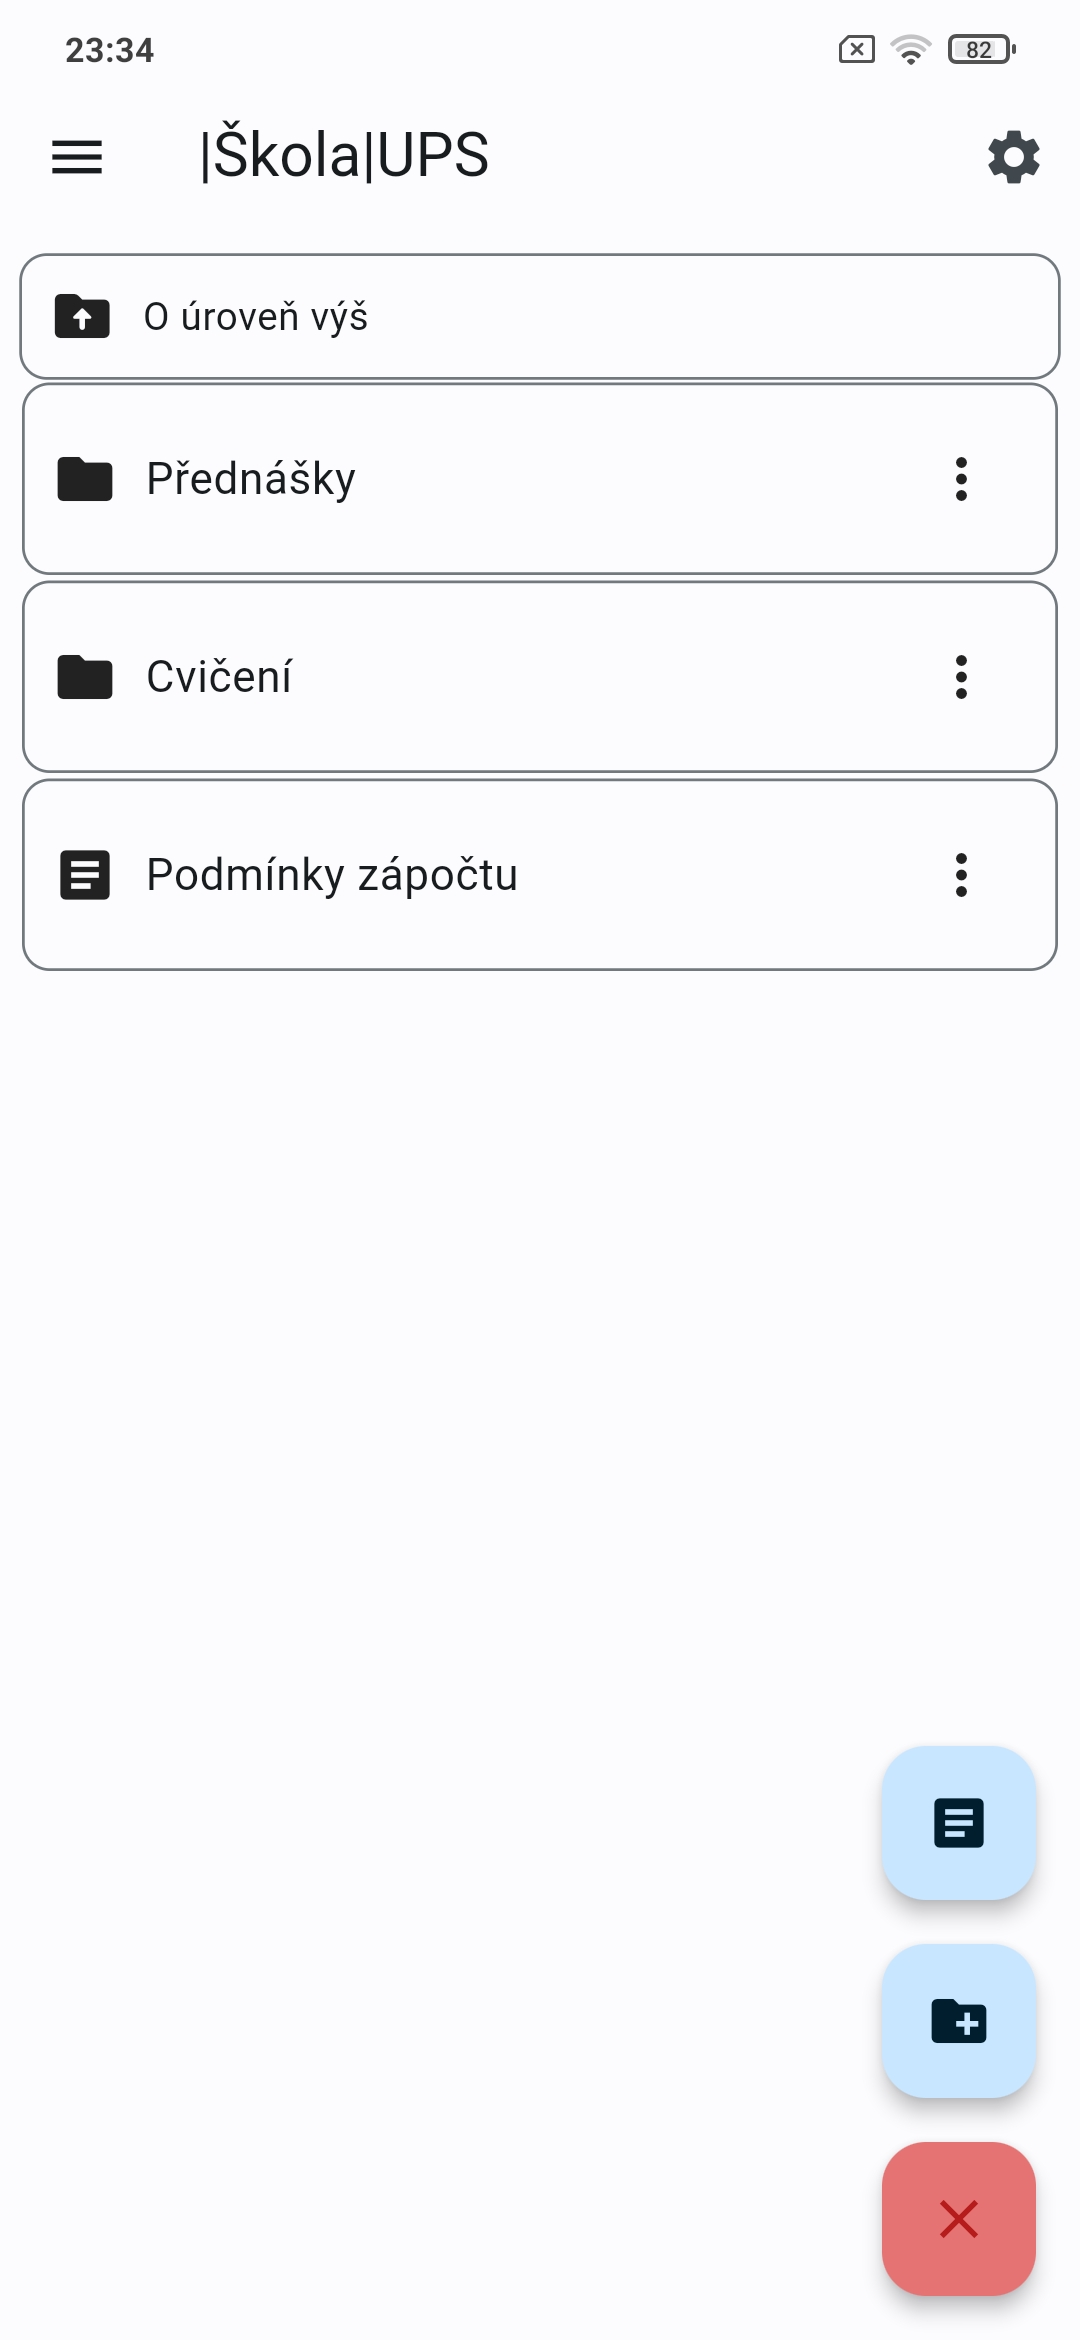
\includegraphics[width=0.53\textwidth]{img/BP-Runt/UserManual/Folder.jpg}
  \caption{Snímek obrazovky, která zobrazuje obsah adresáře formou seznamu}
  \label{fig:FolderScreen}
\end{figure}

\section{Editace poznámky} \label{manual:note}
Na dalších snímcích \ref{fig:editationOfNote} je zobrazen editor formátovaného textu. V aplikačním panelu má uživatel informaci o tom, jakou poznámku zrovna edituje. Pomocí plovoucího tlačítka má uživatel možnost schovat či zobrazit panel nástrojů.  

\begin{figure}[h!]
  \centering
  \begin{minipage}[h]{0.45\textwidth}
    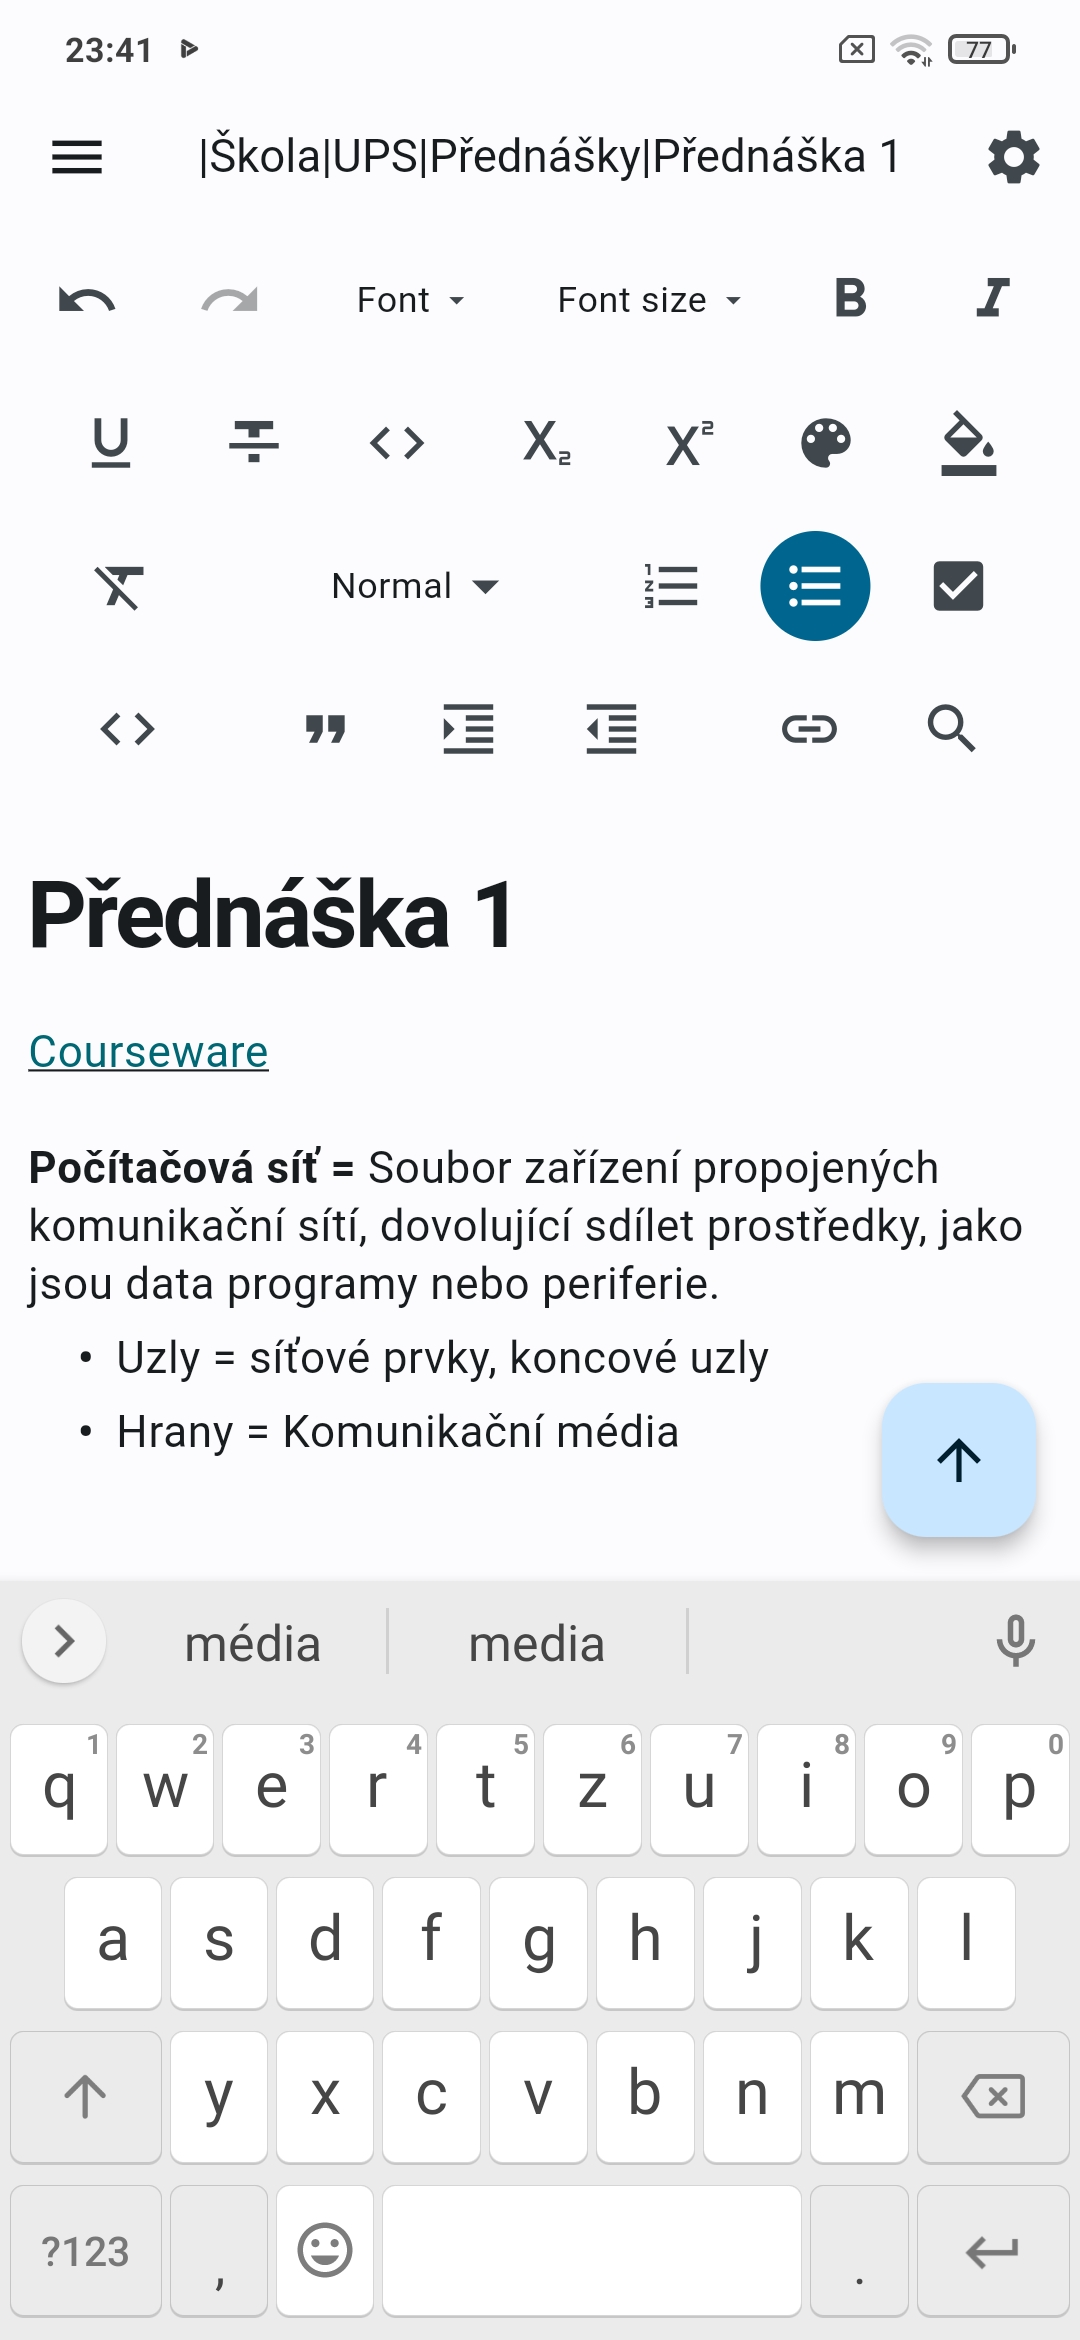
\includegraphics[width=\textwidth]{img/BP-Runt/UserManual/EditingNote.jpg}
  \end{minipage}
  \hspace{10pt}
  \begin{minipage}[h]{0.45\textwidth}
    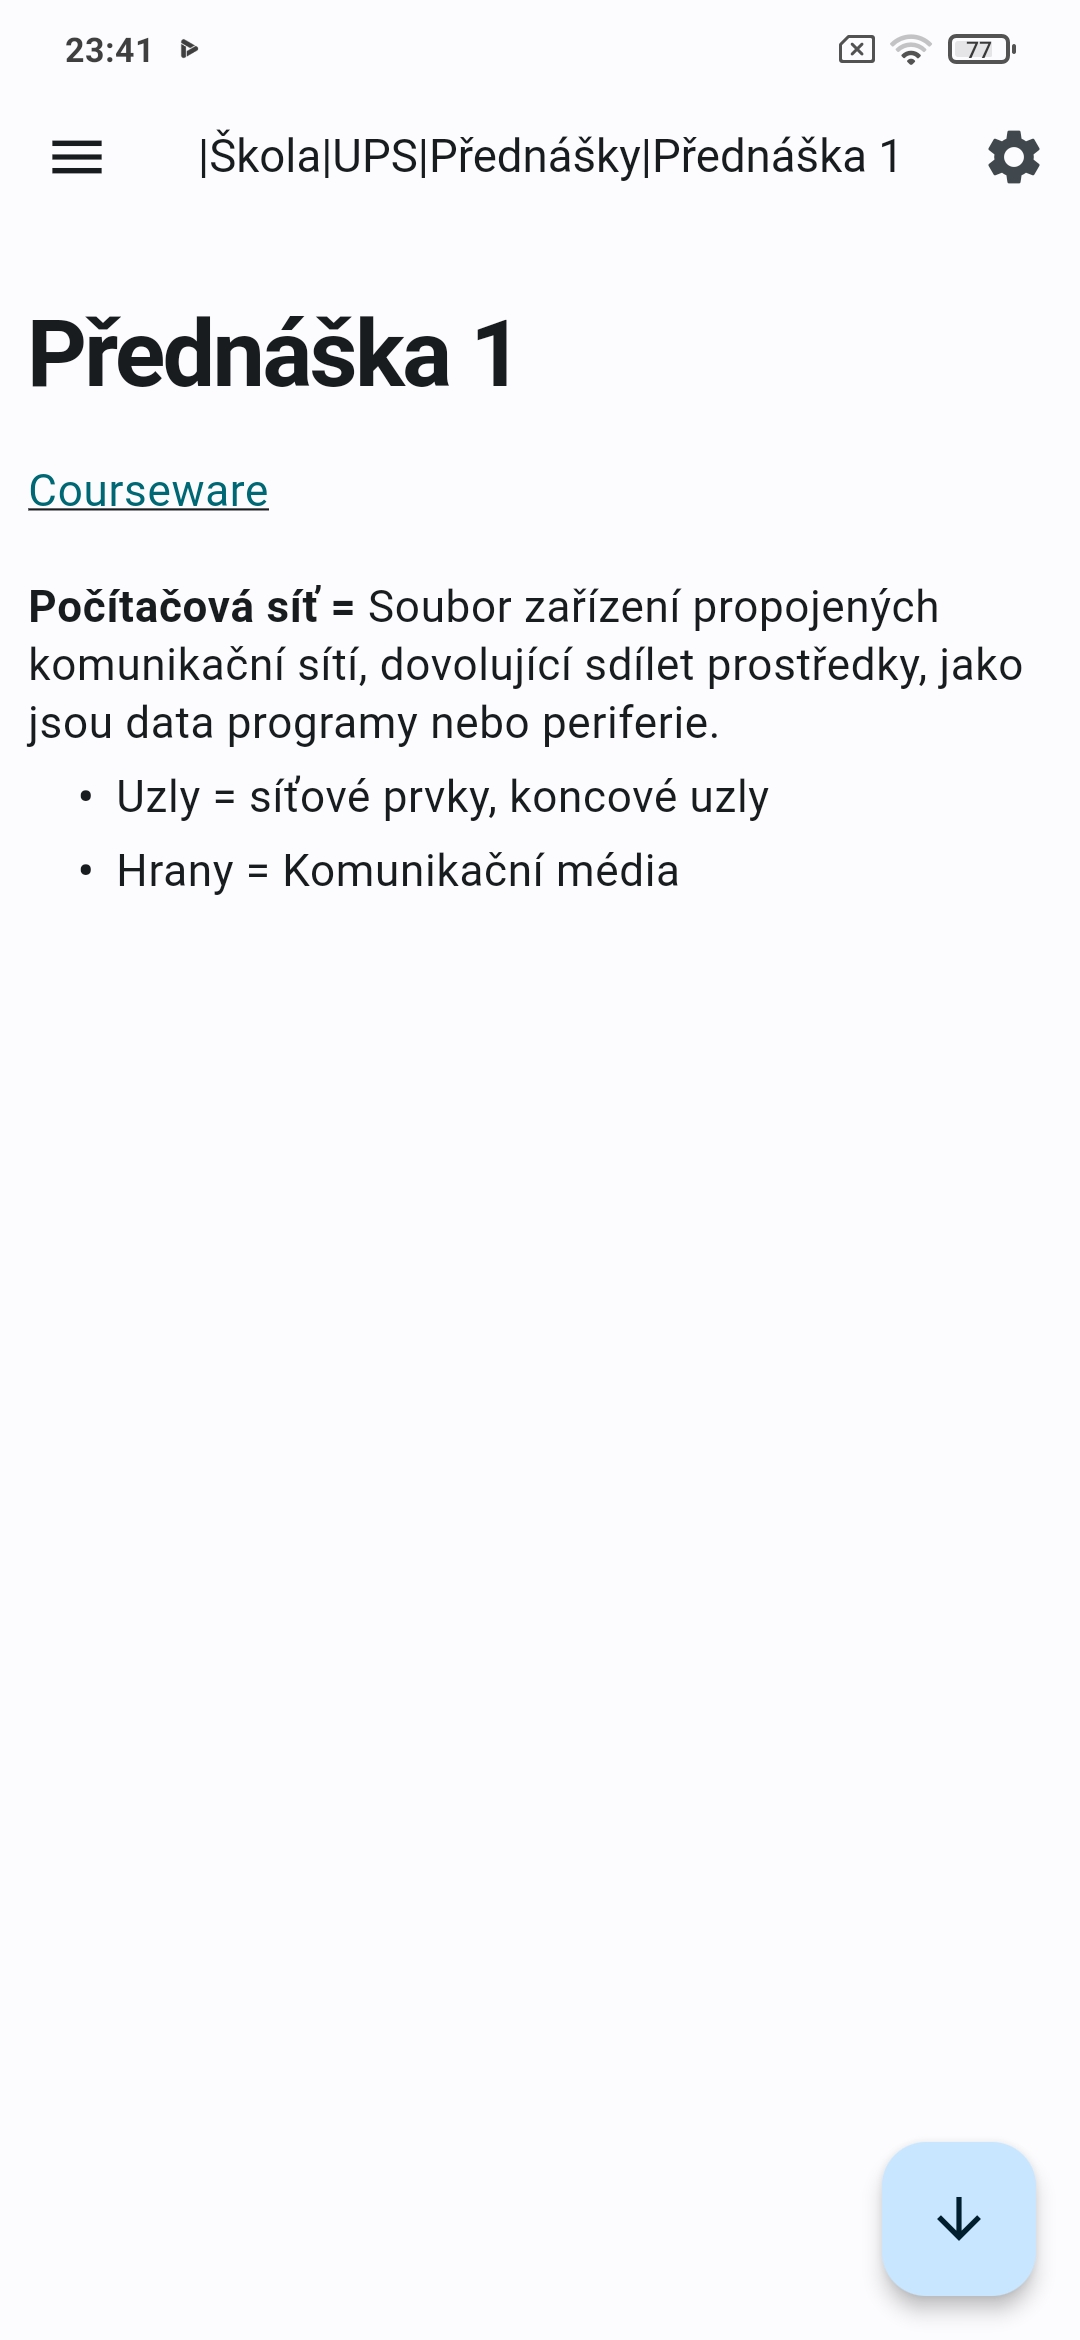
\includegraphics[width=\textwidth]{img/BP-Runt/UserManual/HiddenRichTextEditor.jpg}
  \end{minipage}
  \caption{Obrazovka úpravy poznámky, vlevo s viditelným panelem nástrojů, vpravo se skrytým panelem nástrojů}
  \label{fig:editationOfNote}
\end{figure}

\newpage

\section{Registrace nového uživatele}

Na obrázku \ref{fig:RegisterScreen} se nachází obrazovka pro registraci nového uživatele. Uživatel má možnost se registrovat kombinací e-mailu a hesla nebo pomocí účtu Google. Pokud má uživatel již založený účet, může se pomocí odkazu \textit{Přihlašte se zde!} dostat na~stránku s přihlášením.

\begin{figure}[h!]
  \centering
  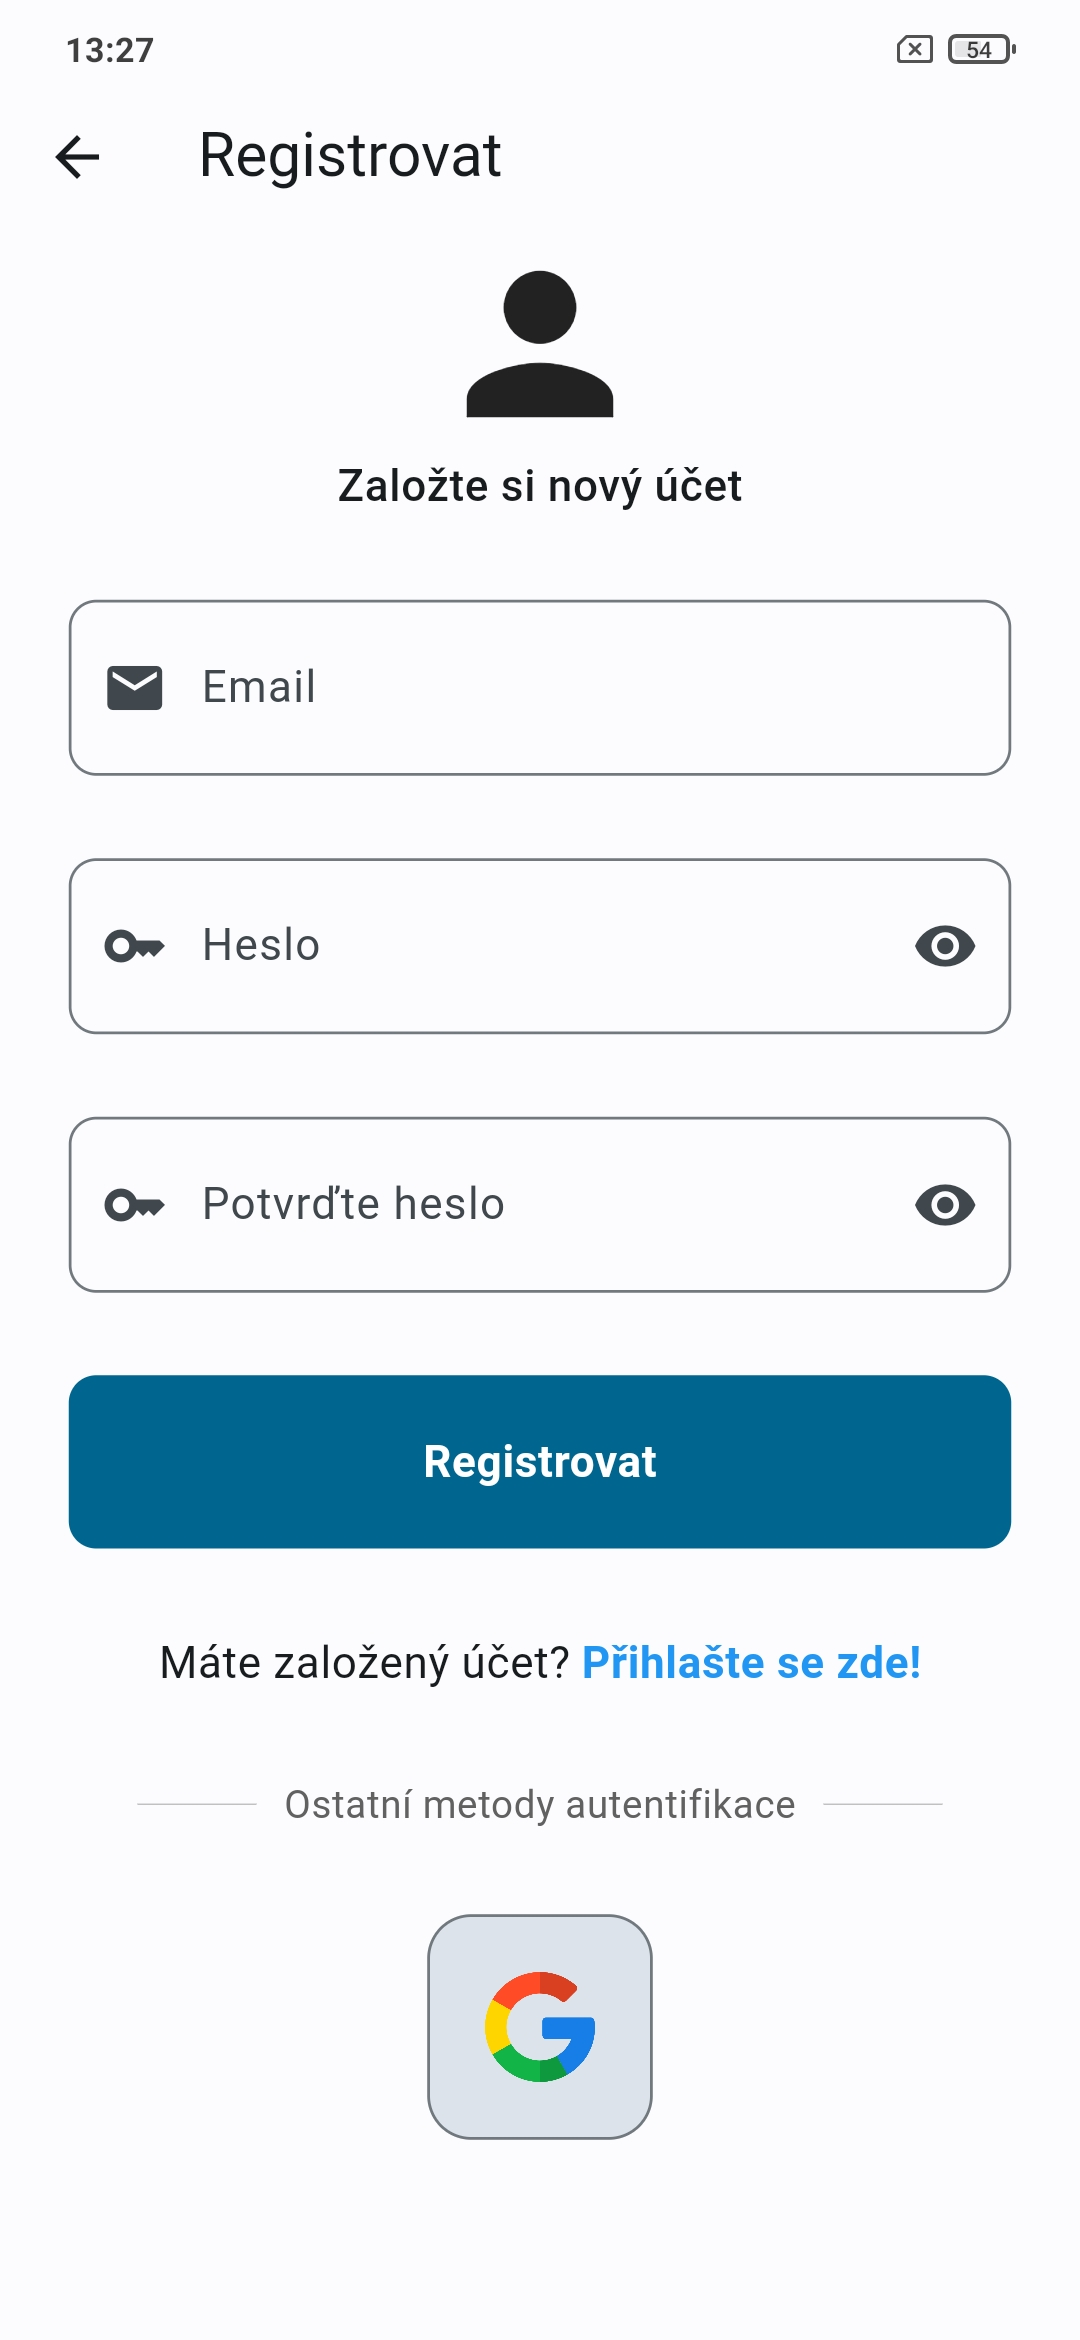
\includegraphics[width=0.55\textwidth]{img/BP-Runt/UserManual/Registration.jpg}
  \caption{Snímek obrazovky pro registraci nového uživatele}
  \label{fig:RegisterScreen}
\end{figure}

\section{Přihlášení uživatele}
Uživatelé se mohou přihlásit buď použitím e-mailu a hesla, nebo prostřednictvím účtu Google. V případě zapomenutí hesla mají uživatelé možnost kliknout na odkaz \textit{Obnovit heslo}, který je přesměruje na stránku pro obnovení hesla. Ti, kteří ještě nemají založený účet, mohou využít odkazu \textit{Založte si nový zde!} pro přesměrování na stránku s registrací. Obrázek \ref{fig:LoginScreen} ukazuje stránku pro přihlášení.
 
\begin{figure}[h!]
  \centering
  \includegraphics[width=0.55\textwidth]{img/BP-Runt/UserManual/LoginPage.jpg}
  \caption{Snímek přihlašovací obrazovky}
  \label{fig:LoginScreen}
\end{figure}

\section{Obnovení hesla}

Na následujícím obrázku \ref{fig:ResetPasswordScreen} se nachází obrazovka pro obnovení hesla. Tato obrazovka obsahuje textové pole pro zadání uživatelova e-mailu a tlačítko, kterým se~odešle e-mail s odkazem pro změnění hesla.

\begin{figure}[h!]
  \centering
  \includegraphics[width=0.6\textwidth]{img/BP-Runt/UserManual/PasswordReset.jpg}
  \caption{Snímek obrazovky pro obnovu hesla}
  \label{fig:ResetPasswordScreen}
\end{figure}

\section{Nastavení} \label{manual:settings}

Na následujícím obrázku \ref{fig:SettinsPage} je zobrazena stránka nastavení. V dalších sekcích bude popsáno, jaké možnosti toto nastavení poskytuje.

\begin{figure}[h!]
  \centering
  \includegraphics[width=0.6\textwidth]{img/BP-Runt/UserManual/Settings.jpg}
  \caption{Snímek obrazovky s nastavením aplikace}
  \label{fig:SettinsPage}
\end{figure}

\subsection{Nastavení jazyka}

Jazyk lze nastavit v nastavení kliknutím na rozbalovací seznam s aktuálním jazykem. Následně je možné si vybrat ze dvou jazyků, a to z češtiny a angličtiny. Přepnutí aplikace do anglického jazyka je ukázáno na obrázku \ref{fig:language}.

\begin{figure}[h!]
  \centering
  \includegraphics[width=0.6\textwidth]{img/BP-Runt/UserManual/Language.jpg}
  \caption{Snímek zobrazující anglickou lokalizaci aplikace}
  \label{fig:language}
\end{figure}

\subsection{Tmavý mód}

Tmavý mód lze v nastavení zapnout pomocí přepínače v řádce \textit{Tmavý mód}. Vzhled tmavého módu je zobrazen na obrázku \ref{fig:DarkMode}.

\begin{figure}[h!]
  \centering
  \includegraphics[width=0.6\textwidth]{img/BP-Runt/UserManual/DarkMode.jpg}
  \caption{Snímek ukazující vzhled tmavého režimu}
  \label{fig:DarkMode}
\end{figure}

\subsection{Zobrazení konfliktů}

Konflikty lze zobrazit kliknutím na tlačítko \textit{ZOBRAZ} v řádku \textit{Zobrazit konflikty}. Na~následujícím obrázku \ref{fig:Conflicts} je zobrazena stránka s konfliktními daty. Konfliktní data jsou zobrazena ve stromovém zobrazení. Každý konflikt má v názvu přesný čas, kdy ke konfliktu došlo. Konfliktní data lze smazat kliknutím na tři tečky a~následným stisknutím možnosti \textit{Smazat}.

\begin{figure}[h!]
  \centering
  \includegraphics[width=0.55\textwidth]{img/BP-Runt/UserManual/Conflicts.jpg}
  \caption{Snímek zobrazující stránku s konfliktními daty}
  \label{fig:Conflicts}
\end{figure}

\subsection{Informace o aplikaci}

Po stisknutí tlačítka \textit{ZOBRAZ} v řádku \textit{Informace o aplikaci} se zobrazí dialogové okno s informacemi o vytvořené aplikaci (viz obrázek \ref{fig:appInformations}), jako je autor, verze aplikace a datum vydání. Na následujícím obrázku je zobrazen snímek dialogového okna s informacemi o~aplikaci.

\begin{figure}[h!]
  \centering
  \includegraphics[width=0.4\textwidth]{img/BP-Runt/UserManual/AppInformations.jpg}
  \caption{Snímek zobrazující stránku s konfliktními daty}
  \label{fig:appInformations}
\end{figure}

\subsection{Webová stránka manuálu}

Při stisknutí tlačítka v řádku \textit{Manuál k aplikaci} je uživatel přesměrován na webovou stránku s manuálem, která je zobrazena v aplikaci. Na obrázku \ref{fig:manualScreen} je tento manuál zobrazen.

\begin{figure}[h!]
  \centering
  \includegraphics[width=0.6\textwidth]{img/BP-Runt/UserManual/Manual.jpg}
  \caption{Snímek zobrazující stránku s webovým zobrazením manuálu}
  \label{fig:manualScreen}
\end{figure}

\chapter{Instalační příručka}\label{app:install-manual}

\section{Android}

Aplikace požaduje minimální verzi Androidu 6.0 Marshmallow (\gls{API} level 23). Pro~nainstalování aplikace na mobilní zařízení je nutné stáhnout nebo překopírovat \gls{APK} soubor aplikace do svého mobilního zařízení. Dalším krokem je vyhledání a~spuštění souboru. Je možné, že mobilní zařízení nebude mít povolené instalování aplikací z~neznámých zdrojů. V tomto případě se zobrazí dialogové okno, ve kterém je nutno povolit instalaci z~neznámých zdrojů. Po spuštění \gls{APK} souboru a povolení instalace z neznámých zdrojů by se mělo zobrazit dialogové okno viz obrázek \ref{fig:instalation-dialog}, ve~kterém stačí zmáčknout tlačítko instalovat a aplikace by se měla nainstalovat.

\begin{figure}[h!]
  \centering
  \includegraphics[width=0.8\textwidth]{img/BP-Runt/Atachment/Notes-instalation.jpg}
  \caption{Instalační dialog}
  \label{fig:instalation-dialog}
\end{figure}

\section{Web}

Webová aplikace je dostupná na adrese: \url{https://note-taking-application-7c5e4.web.app}

Na následujících obrázcích \ref{fig:website-drawer} a \ref{fig:website-login} je zobrazen vzhled webové aplikace.

\begin{figure}[h!]
  \centering
  \includegraphics[width=1\textwidth]{img/BP-Runt/Website/website-drawer.png}
  \caption{Vysunuté menu ve webové verzi aplikace}
  \label{fig:website-drawer}
\end{figure}

\begin{figure}[h!]
  \centering
  \includegraphics[width=1\textwidth]{img/BP-Runt/Website/login-web.png}
  \caption{Přihlašovací stránka ve webové verzi aplikace}
  \label{fig:website-login}
\end{figure}

\chapter{Konfigurace Firebase}\label{app:firebase-configuration}

V následující příloze se nachází příručka, jak založit, konfigurovat a propojit Firebase projekt s Flutter aplikací.

\section{Vytvoření Firebase projektu}

Pro vytvoření projektu se musíme na stránce Firebase\footnote{https://firebase.google.com/} přihlásit účtem Google. Po~přihlášení klikneme na tlačítko pro založení nového projektu viz obrázek \ref{fig:firebase-new-project}. 

\begin{figure}[h!]
  \centering
  \includegraphics[width=1\textwidth]{img/BP-Runt/firebase-configuration/new-firebase-project.png}
  \caption{Založení nového projektu}
  \label{fig:firebase-new-project}
\end{figure}

Vyplníme jméno projektu a stiskneme tlačítko \textit{Next}. Na další stránce je nastavení Google Analytics, které můžeme zapnout nebo jej nechat vypnuté. Po vytvoření projektu se budeme nacházet na hlavní stránce projektu.

\section{Propojení Firebase s Flutter projektem} \label{sec:flutter-connection}

Firebase projekt lze s Flutter projektem propojit různými způsoby. Následující návod se řídí instrukcemi z oficiální dokumentace\footnote{https://firebase.google.com/docs/flutter/setup?platform=android}. Otevřeme hlavní stránku projektu, kde nalezneme logo Flutteru. Stiskneme logo Flutteru. Zobrazí se návod, dle kterého budeme dále postupovat:

\begin{enumerate}[label=\arabic*.]
    \item Nainstalujeme na své zařízení Firebase \gls{CLI}. Návod na instalaci: \url{https://firebase.google.com/docs/cli#setup_update_cli},
    \item Otevřeme příkazovou řádku a zadáme příkaz: \texttt{firebase login},
    \item Přihlásíme se účtem Google, na kterém máme založený projekt, který chceme propojit s naší aplikací,
    \item Zadáme příkaz: \texttt{dart pub global activate flutterfire\_cli},
    \item Zadáme příkaz: \texttt{flutterfire configure},
    \item Objeví se všechny Firebase projekty, které máme na našem účtu založeny. Vybereme ten, který chceme propojit s naší aplikací,
    \item Zobrazí se seznam platforem, na které můžeme Firebase konfigurovat. Při~stisknutí klávesy enter se konfigurují všechny zobrazené platformy,
    \item Spojení by se mělo automaticky konfigurovat. V adresáři \texttt{lib/} by se měl vytvořit soubor \texttt{firebase\_options.dart}. Na hlavní stránce Firebase projektu by se mělo objevit propojení s platformou webu, Androidu, macOS a~iOS viz obrázek \ref{fig:firebase-connection},
    \item Pro dokončení spojení s webovou aplikací je nutné změnit ve zdrojovém kódu \texttt{main.dart} část definující spojení s webovou aplikací viz zdrojový kód \ref{code:web-configuration}. Do této části kódu je nutno doplnit konfigurační údaje, které získáme v~nastavení webového spojení viz obrázek \ref{fig:firebase-web-configuration}.
\end{enumerate}

\begin{figure}[h!]
  \centering
  \includegraphics[width=1\textwidth]{img/BP-Runt/firebase-configuration/firebase-connection.png}
  \caption{Úspěšné propojení s aplikací}
  \label{fig:firebase-connection}
\end{figure}

\begin{code}{java}{Konfigurace propojení s webovou aplikací \label{code:web-configuration}}
if (kIsWeb) {
      await Firebase.initializeApp(
        options: const FirebaseOptions(
          apiKey: "<vaše-apikey>",
          appId: "<vaše-appId>",
          messagingSenderId: "<vaše-messageSenderId>",
          projectId: "<vaše-projectId>",
        ),
      );
    }
\end{code}

\begin{figure}[h!]
  \centering
  \includegraphics[width=1\textwidth]{img/BP-Runt/firebase-configuration/configuration-data-web.png}
  \caption{Konfigurační údaje webové aplikace}
  \label{fig:firebase-web-configuration}
\end{figure}

\section{Firebase Authentication}

Následující část se zabývá nastavením autentizačních služeb projektu Firebase. Vyvíjená aplikace využívá k autentizaci uživatele kombinací e-mailu a hesla a prostřednictvím účtu Google viz obrázek \ref{fig:auth-providers}. Obě metody budeme muset nastavit.

\begin{figure}[h!]
  \centering
  \includegraphics[width=1\textwidth]{img/BP-Runt/firebase-configuration/firebase-auth-providers.png}
  \caption{Způsoby autentizace}
  \label{fig:auth-providers}
\end{figure}

\subsection{Autentizace e-mailem a heslem}

\begin{enumerate}[label=\arabic*.]
    \item Klikneme na přidání nového způsobu ověření identity a zvolíme způsob e-mailu a hesla,
    \item Povolíme tento způsob a klikneme na tlačítko \textit{Save} viz obrázek \ref{fig:email-and-password},
    \item Způsob ověření kombinací e-mailem a heslem by se měl objevit mezi povolenými způsoby.
\end{enumerate}

\begin{figure}[h!]
  \centering
  \includegraphics[width=1\textwidth]{img/BP-Runt/firebase-configuration/auth-email-and-password.png}
  \caption{Povolení autentizace pomocí e-mailu a hesla}
  \label{fig:email-and-password}
\end{figure}

\subsection{Autentizace účtem Google}

Následující sekce poskytuje postup, jak lze nastavit autentizaci pomocí účtu Google:

\begin{enumerate}
    \item Ve vašem Firebase projektu se přesuňte do nastavení autentizace. Zde přidejte nový způsob autentizace účtem Google. Zobrazí se dialog, ve kterém je tuto metodu ověření nutno povolit viz obrázek \ref{fig:enabling-google-sign-in},  

    \begin{figure}[h!]
    \centering
    \includegraphics[width=1\textwidth]{img/BP-Runt/firebase-configuration/google-sign-in/enabling-google-sign-in.png}
    \caption{Povolení ověření identity prostřednictvím účtu Google}
    \label{fig:enabling-google-sign-in}
    \end{figure}

    \item Otevřete nastavení propojení s Android aplikací a nastavte otisk certifikátů \gls{SHA}-1:
      \begin{enumerate}
        \item Otevřeme konzoli a zadáme příkaz: \newline\noindent\texttt{keytool -list -v -alias androiddebugkey -keystore \newline \%USERPROFILE\%/.android/debug.keystore},
        \item Jako heslo zvolíme: \texttt{android},
        \item Tento příkaz vygeneruje otisky \gls{SHA}-1 a \gls{SHA}-256,
        V nastavení propojení pak stiskneme tlačítko Add fingerprint viz obrázek \ref{fig:add-fingerprint},
        \item Zobrazí se dialogové okno, do kterého zkopírujeme vygenerované otisky \gls{SHA}-1 a \gls{SHA}-256 viz obrázek \ref{fig:fingerprint}. 

        \begin{figure}[h!]
    \centering
    \includegraphics[width=1\textwidth]{img/BP-Runt/firebase-configuration/google-sign-in/adding-fingerprint.png}
    \caption{Přidání \gls{SHA} certifikátů}
    \label{fig:add-fingerprint}
    \end{figure}

    \begin{figure}[h!]
    \centering
    \includegraphics[width=1\textwidth]{img/BP-Runt/firebase-configuration/google-sign-in/fingerprint.png}
    \caption{Zadání otisku do dialogového okna}
    \label{fig:fingerprint}
    \end{figure}
    
    \end{enumerate}
    
\end{enumerate}

\newpage

\section{Firebase Firestore}

Tato sekce poskytuje návod, jak vytvořit a nakonfigurovat databázi Firestore k ukládání uživatelských dat:

\begin{enumerate}[label=\arabic*.]
\item Vytvořte databázi ve svém Firebase projektu. Objeví se dialogové okno, ve~kterém zvolte server, na kterém budou data uložena (viz obrázek \ref{fig:firestore-configuration-01}) a stiskněte tlačítko \textit{Next}. Na další stránce zvolte \textit{Start in production mode} (viz obrázek \ref{fig:firestore-configuration-02}) a volbu potvrďte stiskem tlačítka \textit{Create}, 

\begin{figure}[h!]
  \centering
  \includegraphics[width=1\textwidth]{img/BP-Runt/firebase-configuration/firestore/create-firestore-database.png}
  \caption{Založení Firestore databáze - volba serveru}
  \label{fig:firestore-configuration-01}
\end{figure}

\begin{figure}[h!]
  \centering
  \includegraphics[width=1\textwidth]{img/BP-Runt/firebase-configuration/firestore/create-firestore-database-2.png}
  \caption{Založení Firestore databáze - založení v produkčním módu}
  \label{fig:firestore-configuration-02}
\end{figure}

\item Vytvořená databáze není připravena pro čtení a zápis dat. Je potřeba upravit pravidla (\textit{Rules}) a povolit čtení a zápis dat viz zdrojový kód \ref{code:firestore-rules}. 

\begin{code}{java}{Nastavení pravidel databáze Firestore \label{code:firestore-rules}}
rules_version = '2';

service cloud.firestore {
  match /databases/{database}/documents {
    match /{document=**} {
      allow read, write: if request.auth != null;
    }
  }
}
\end{code}

\end{enumerate}

\section{Firebase Hosting}

Následující část příručky obsahuje návod, jak vytvořit hosting pro webové aplikace, které byly vytvořeny technologií Flutter. Předpokladem tohoto návodu je vytvořený a spárovaný Firebase projekt a nainstalované Firebase \gls{CLI}:

\begin{enumerate}[label=\arabic*.]
    \item Otevřete příkazovou řádku v kořenovém adresáři Flutter projektu a vytvořte build webové aplikace příkazem: \texttt{flutter build web}. \newline Tento build se uloží do složky \texttt{build/web}, 
    \item Dále je potřeba nastavit hostování pro váš projekt na webových stránkách Firebase. Ujistěte se, že vaše webová aplikace je propojena s projektem Firebase. Pokud není, konfigurujte spojení dle návodu \ref{sec:flutter-connection}. Pokud toto propojení existuje, přejděte do nastavení webové aplikace a zvolte hosting, na který bude web odkazovat. Tento postup je zobrazen na obrázcích \ref{fig:enabling-hosting} a \ref{fig:link-hosting-web},
    \begin{figure}[h!]
  \centering
  \includegraphics[width=1\textwidth]{img/BP-Runt/firebase-configuration/hosting/Firebase-enable-hosting.png}
  \caption{Tlačítko nastavení hostingu v nastavení webové aplikace}
  \label{fig:enabling-hosting}
\end{figure}
\begin{figure}[h!]
  \centering
  \includegraphics[width=0.6\textwidth]{img/BP-Runt/firebase-configuration/hosting/Link-to-hosting-site.png}
  \caption{Volba hostingu, na který bude web odkazovat}
  \label{fig:link-hosting-web}
\end{figure}

\item Přesuňte se zpět do příkazové řádky a přesvědčte se, že jste přihlášeni k Firebase příkazem \texttt{firebase login}. Případně se přihlaste účtem Google, který používáte,
\item Pomocí příkazu: \texttt{firebase init hosting} proveďte inicializaci hostování, 
\item Předchozí příkaz vytvoří ve Flutter projektu soubor \texttt{firebase.json} viz zdrojový kód \ref{code:firebase-json}. V tomto souboru nastavte hodnotu klíče "public" na cestu k~buildu webu, který jsme vytvořili v prvním kroku,

\newpage

\begin{code}{java}{Konfigurace propojení s webovou aplikací \label{code:firebase-json}}
{
  "hosting": {
    "public": "build/web",
    "ignore": [
      "firebase.json",
      "**/.*",
      "**/node_modules/**"
    ],
    "rewrites": [
      {
        "source": "**",
        "destination": "/index.html"
      }
    ]
  }
}
\end{code}

\item Proveďte nasazení aplikace na Firebase Hosting příkazem: \texttt{firebase deploy}. Po dokončení nasazení se automaticky vygeneruje \gls{URL} adresa, na které bude vaše webová aplikace dostupná.

\end{enumerate}


\chapter{Obsah ZIP souboru}

\dirtree{%
  .1 A20B0226P\_prilohy.
  .2 Text\_prace.
  .3 LaTeX\_zdrojove\_soubory\DTcomment{Zdrojové soubory \gls{PDF}}.
  .3 A20B0226P\_BP.pdf\DTcomment{\gls{PDF} verze bakalářské práce}.
  .2 Aplikace\_a\_knihovny.
  .3 Notes\_zdrojove\_soubory\DTcomment{Zdrojové soubory aplikace}. 
  .3 Notes.apk\DTcomment{Instalační soubor aplikace}.
  .3 Dartdoc\DTcomment{Dokumentace zdrojového kódu}.
  .3 Navod\_na\_sestaveni.txt\DTcomment{Návod na sestavení aplikace}.
  .3 Manual\_zdrojove\_soubory\DTcomment{Zdrojové soubory webové stránky manuálu}.
  .2 Readme.txt\DTcomment{Detailní informace o obsahu adresáře}.
}


% _____________________________________________________________________________
%
%		BACK COVER
% _____________________________________________________________________________
%
%\setbackpagesign{img/qr-code}
\backpage
\end{document}